In diesem Kapitel wird erläutert, wie die Ideen aus Kapitel \ref{konzept} in die Praxis umgesetzt wurden und welche Abstriche dabei erforderlich waren. Dazu wird zunächst beschrieben, wie die Messumgebung, der MCTS-Agent und der PPO-Agent implementiert wurden. Anschließend wird dargestellt, wie die Szenarien zur Untersuchung der Robustheit der implementierten Agenten abgebildet werden. Der gesamte im Rahmen dieser Arbeit entstandene Quellcode ist auf GitHub unter \url{https://github.com/LeoHerrmann/connect_four_robustness/releases/tag/v1.0.0} einsehbar.

\subsection{Messumgebung}

\label{messumgebung}

% PettingZoo-Bibliothek

Als Grundlage für die Messumgebung dient die Open Source Python-Bibliothek PettingZoo der Farama Foundation, die zum Entwickeln und Testen von MARL-Systemen konzipiert wurde. Sie stellt eine einheitliche Schnittstelle zu Umgebungen bereit, in der Agenten miteinander interagieren können. Die Schnittstelle ähnelt dabei der Schnittstelle des Frameworks Gymnasium des selben Herausgebers, das Single-Agent-Umgebungen bereitstellt.

Die Umgebungen definieren den Rahmen, in dem die Agenten miteinander interagieren. Sie weisen ein bestimmtes Verhalten auf und definieren unter anderem, unter welchen Bedingungen welche Aktionen möglich sind, Belohnungen verteilt werden und in welcher Form die Agenten Informationen über den Zustand der Umgebung erhalten. Es existieren eine Reihe von vorgefertigten Umgebungen, darunter welche, die kooperative Probleme zum Benchmarking von MARL-Systemen oder auch rundenbasierte Spiele wie Vier Gewinnt abbilden.

Die durch PettingZoo bereitgestellte Schnittstelle ermöglicht es, aus Sicht eines Agenten den aktuellen Zustand der Umgebung zu beobachten, die im aktuellen Zustand möglichen Aktionen und erhaltenen Belohnungen zu ermitteln und eine Aktion auszuwählen, die in der Umgebung durchgeführt werden soll.

Für alle Agenten der Umgebung kann benutzerdefinierte Logik eingebunden werden, die bestimmt, wie sie ihre Aktionen wählen. Vorgesehen sind dabei RL-Modelle, es können jedoch auch symbolische Algorithmen eingesetzt werden, darunter auch welche, die ihre Entscheidungen rein zufällig oder unter Einbezug von menschlichen Eingaben treffen \cite{Farama.2025}.

% Implementierung der Messumgebung

Die Implementierung der Messumgebung baut auf der offiziellen Implementierung der Vier-Gewinnt-Umgebung von PettingZoo auf. Die Messumgebung tut dabei nichts anderes, als wiederholt zwei Agenten mit bestimmten Lösungsansätzen das Spiel spielen zu lassen und dabei die Gewinnraten und Spieldauer aufzuzeichnen. Die Open-Source-Eigenschaft von PettingZoo ermöglicht es, den Quellcode der Umgebung zu modifizieren. Davon wird im weiteren Verlauf der Arbeit Gebrauch gemacht, unter anderem, um die verschiedenen Szenarien zur Untersuchung von Robustheit abzubilden.

Im Zuge der Realisierung der Messumgebung ist aufgefallen, dass wenn zwei Agenten (Spieler 0 und Spieler 1) alle Aktionen im Spiel mit derselben Wahrscheinlichkeit rein zufällig wählen, nach 1000 Spielen durch Spieler 0 mit 55,3 \% eine wesentlich höhere Gewinnrate erzielt wird als durch Spieler 1 mit 44,5 \%. Der in \ref{fig:f1} abgebildete gegenläufige Verlauf der Gewinnrate über die Anzahl der durchgeführten Spiele zeigt, dass das Spielergebnis selten unentschieden ist.

Um sicherzustellen, dass es sich bei der Differenz in der Gewinnrate nicht um einen stochastisch bedingten Messfehler handelt, wurde ein Binomialtest durchgeführt. Bei gleichen Chancen für beide Spieler wird eine Gewinnrate von jeweils 50 \% erwartet. Der Test mit $n = 998$ entschiedenen Spielen, wovon $k = 553$ durch den ersten Spieler gewonnen wurden, liefert unter der Hypothese, dass die beiden Spieler gleiche Chancen haben, p-Werte von 0,0007, was unter dem Signifikanzniveau von $\alpha = 0,05$ liegt. Dadurch wird die Hypothese verworfen, was bedeutet, dass die Differenz der Gewinnraten trotz stochastischer Schwankungen signifikant ist.

\begin{figure}[ht!]%[!tbp]
	\begin{subfigure}[b]{0.48\textwidth}
		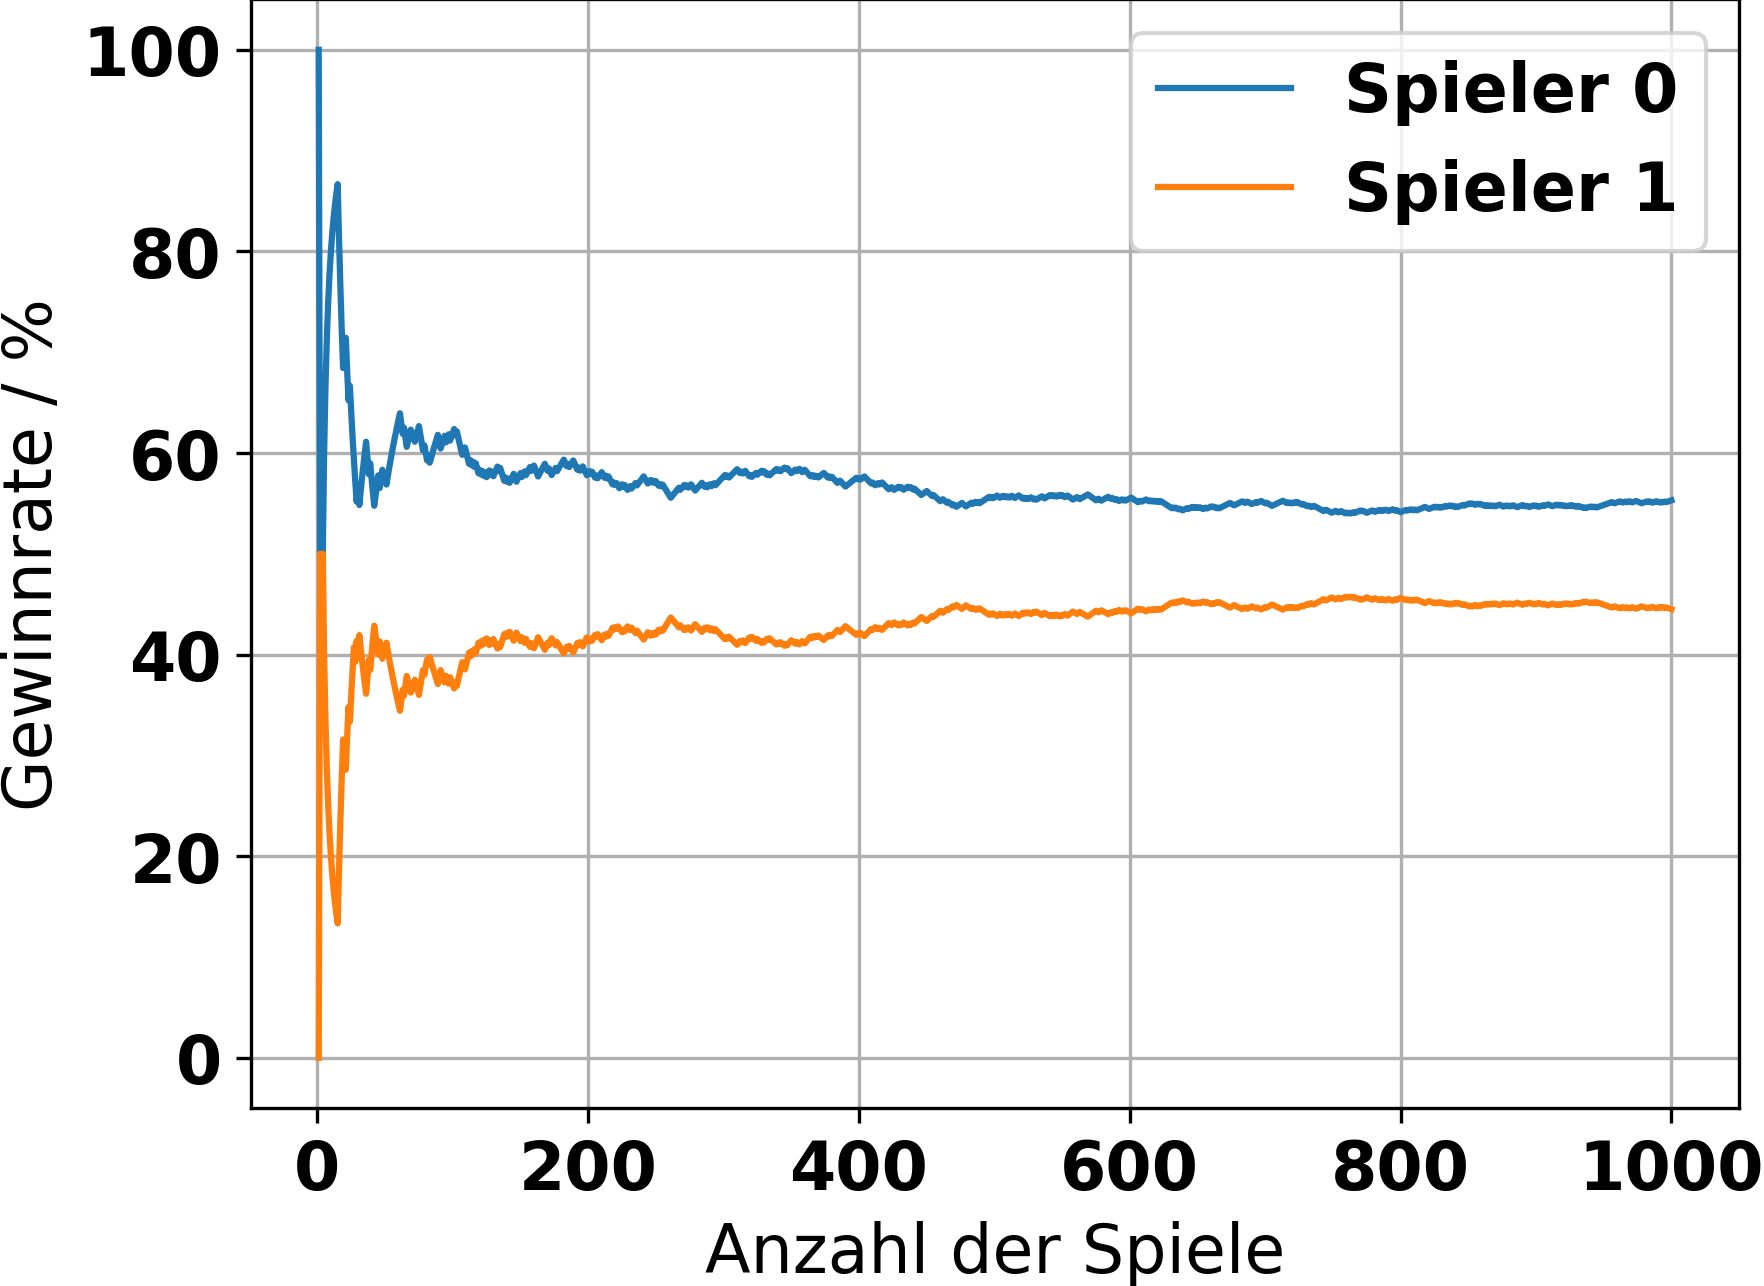
\includegraphics[width=\textwidth]{Bilder/random_vs_random_constant_player_order_graph_win_rates.png}
		\caption{Gewinnrate.}
		\label{fig:f1}
	\end{subfigure}
	\hfill
	\begin{subfigure}[b]{0.48\textwidth}
		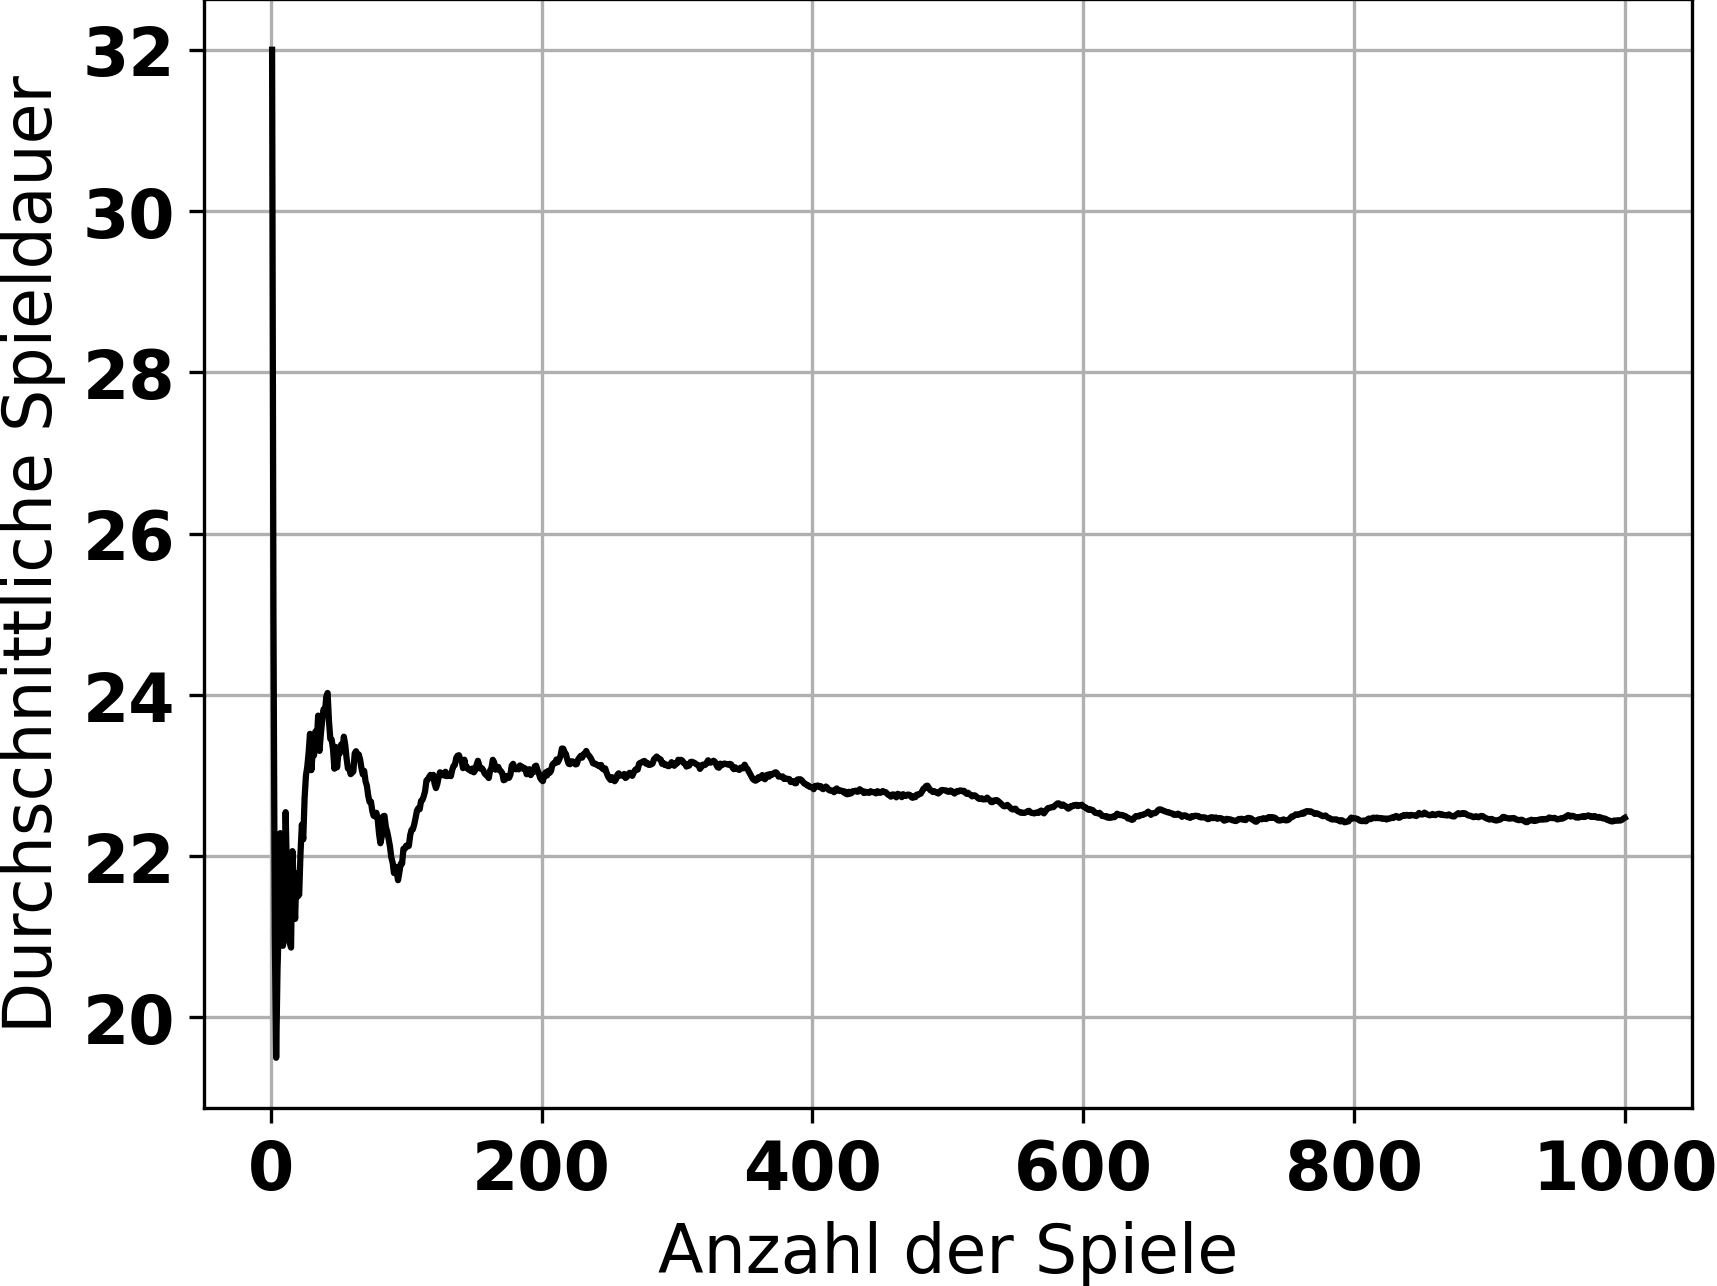
\includegraphics[width=\textwidth]{Bilder/random_vs_random_constant_player_order_graph_game_length.png}
		\caption{Durchschnittliche Spieldauer.}
		\label{fig:f2}
	\end{subfigure}
	\caption{Gewinnrate und durchschnittliche Spieldauer bei konstanter Spielerreihenfolge.}
\end{figure}

Das lässt sich dadurch erklären, dass die Vier-Gewinnt-Umgebung so implementiert ist, dass Spieler 0 immer der Spieler ist, der den ersten Stein setzen darf. Er ist damit seinem Gegenspieler immer einen Spielzug voraus, was die Wahrscheinlichkeit erhöht, als erstes Vier Steine in eine Reihe zu bekommen. An dieser Stelle sei nochmals zu erwähnen, dass bei Vier Gewinnt der erste Spieler bei optimaler Spielweise stets gewinnen kann. Um ausgeglichene Messungen zu gewährleisten, muss daher sichergestellt werden, dass sich im Rahmen der Messungen die beiden Spieler mit dem ersten Zug abwechseln.

Die Vier-Gewinnt-Umgebung von PettingZoo wurde daher erweitert, um einen Parameter entgegenzunehmen und zu verarbeiten, der bestimmt, welcher Spieler anfangen soll. Die Messumgebung wechselt den Wert des Parameters nach jedem Spiel durch. Nach dieser Änderung weisen die Spiele wesentlich ausgeglichenere Ergebnisse auf. 48,6 \% der Spiele werden durch Spieler 0 gewonnen und 51,3 \% durch Spieler 1. Der zuvor bereits durchgeführte Binomialtest liefert mit den Werten $n = 999$, $k = 486$ einen p-Wert von 0,41, was deutlich über dem Signifikanzniveau von $\alpha = 0,05$ liegt, wodurch die Hypothese behalten wird. Die durchschnittliche Spieldauer bleibt dabei mit 22,45 Zügen (95 \%-CI: 22,00 - 22,90) vor der Änderung gegenüber 22,60 Zügen (95 \%-CI: 22,14 - 23,05) nach der Änderung abgesehen von den stochastisch bedingten Schwankungen nahezu unverändert.

\begin{figure}[ht!]%[!tbp]
	\begin{subfigure}[b]{0.48\textwidth}
		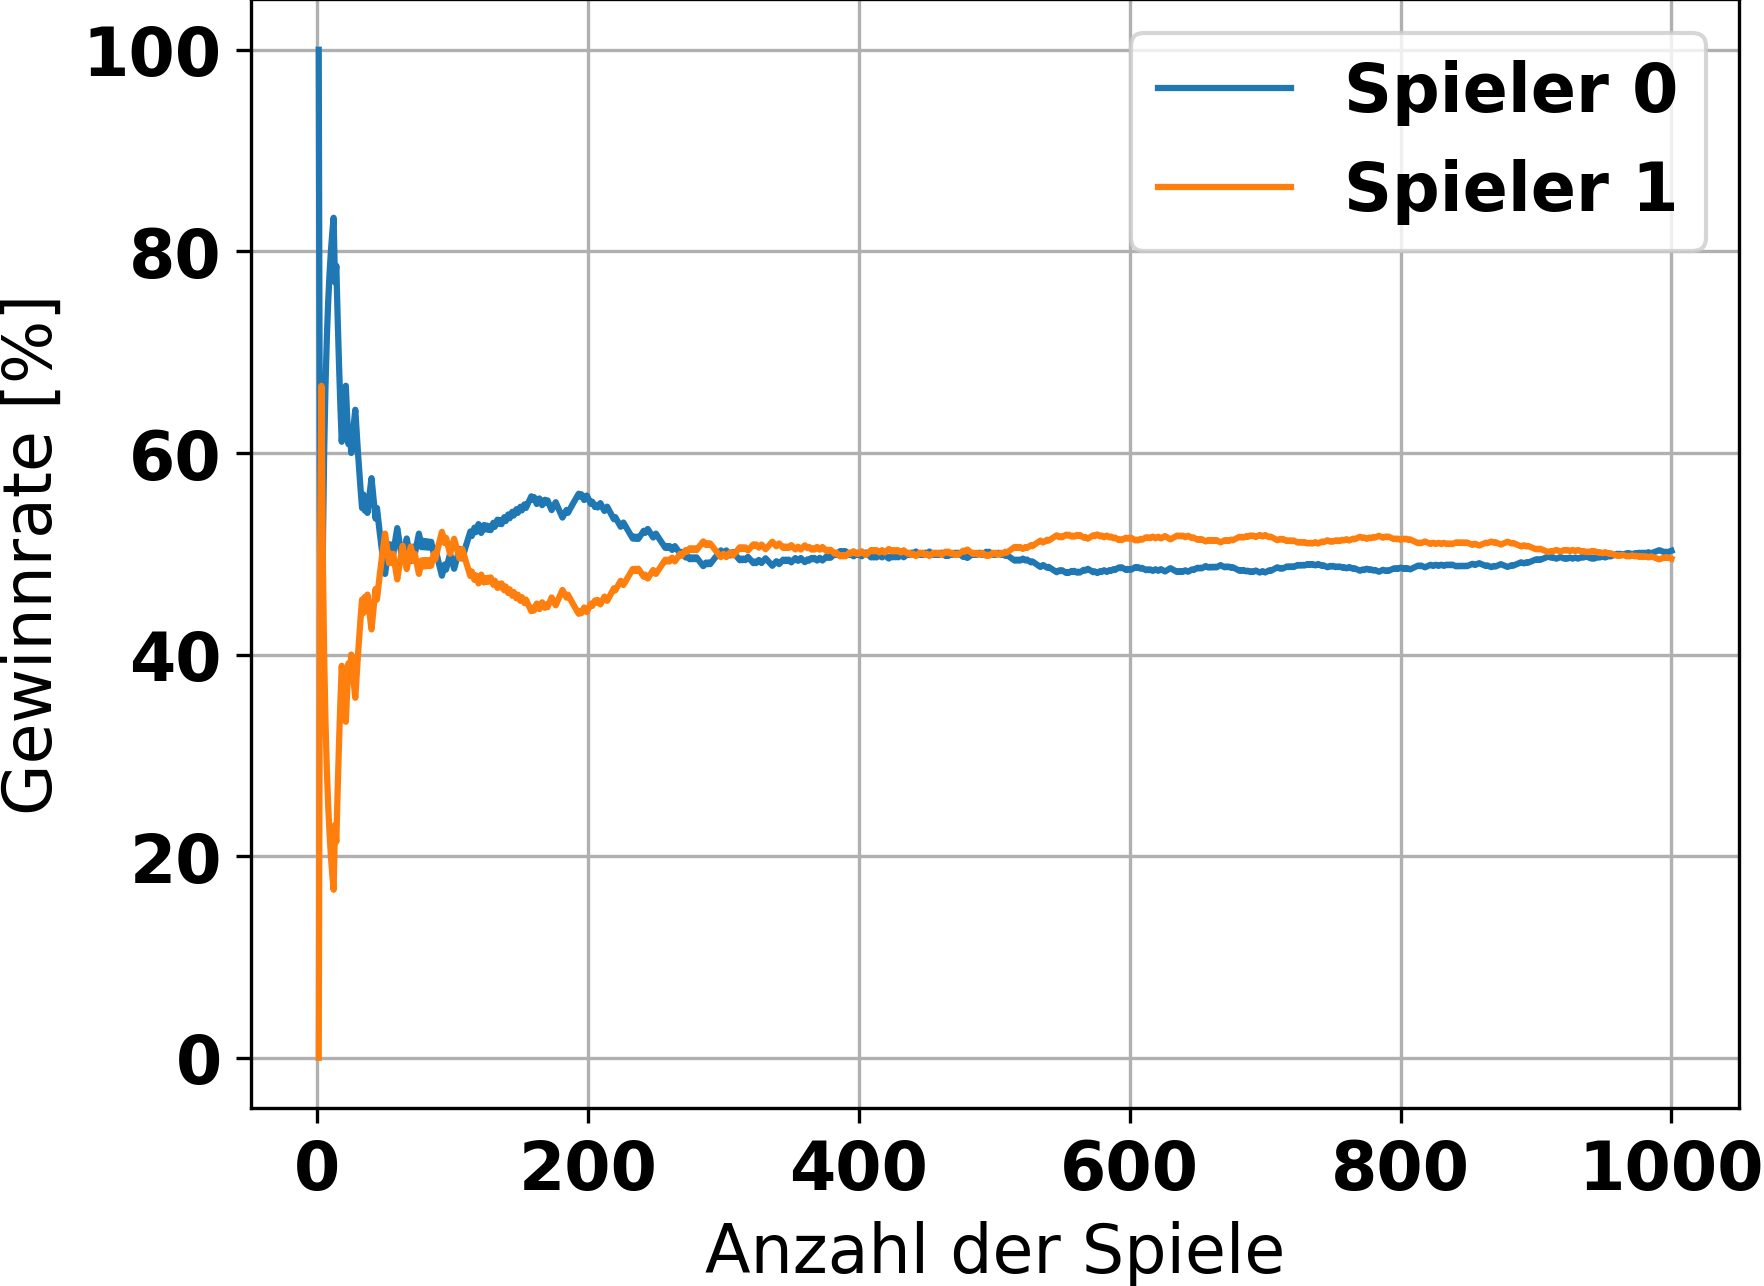
\includegraphics[width=\textwidth]{Bilder/random_vs_random_alternating_player_order_graph_win_rates.png}
		\caption{Gewinnrate.}
		\label{fig:f3}
	\end{subfigure}
	\hfill
	\begin{subfigure}[b]{0.48\textwidth}
		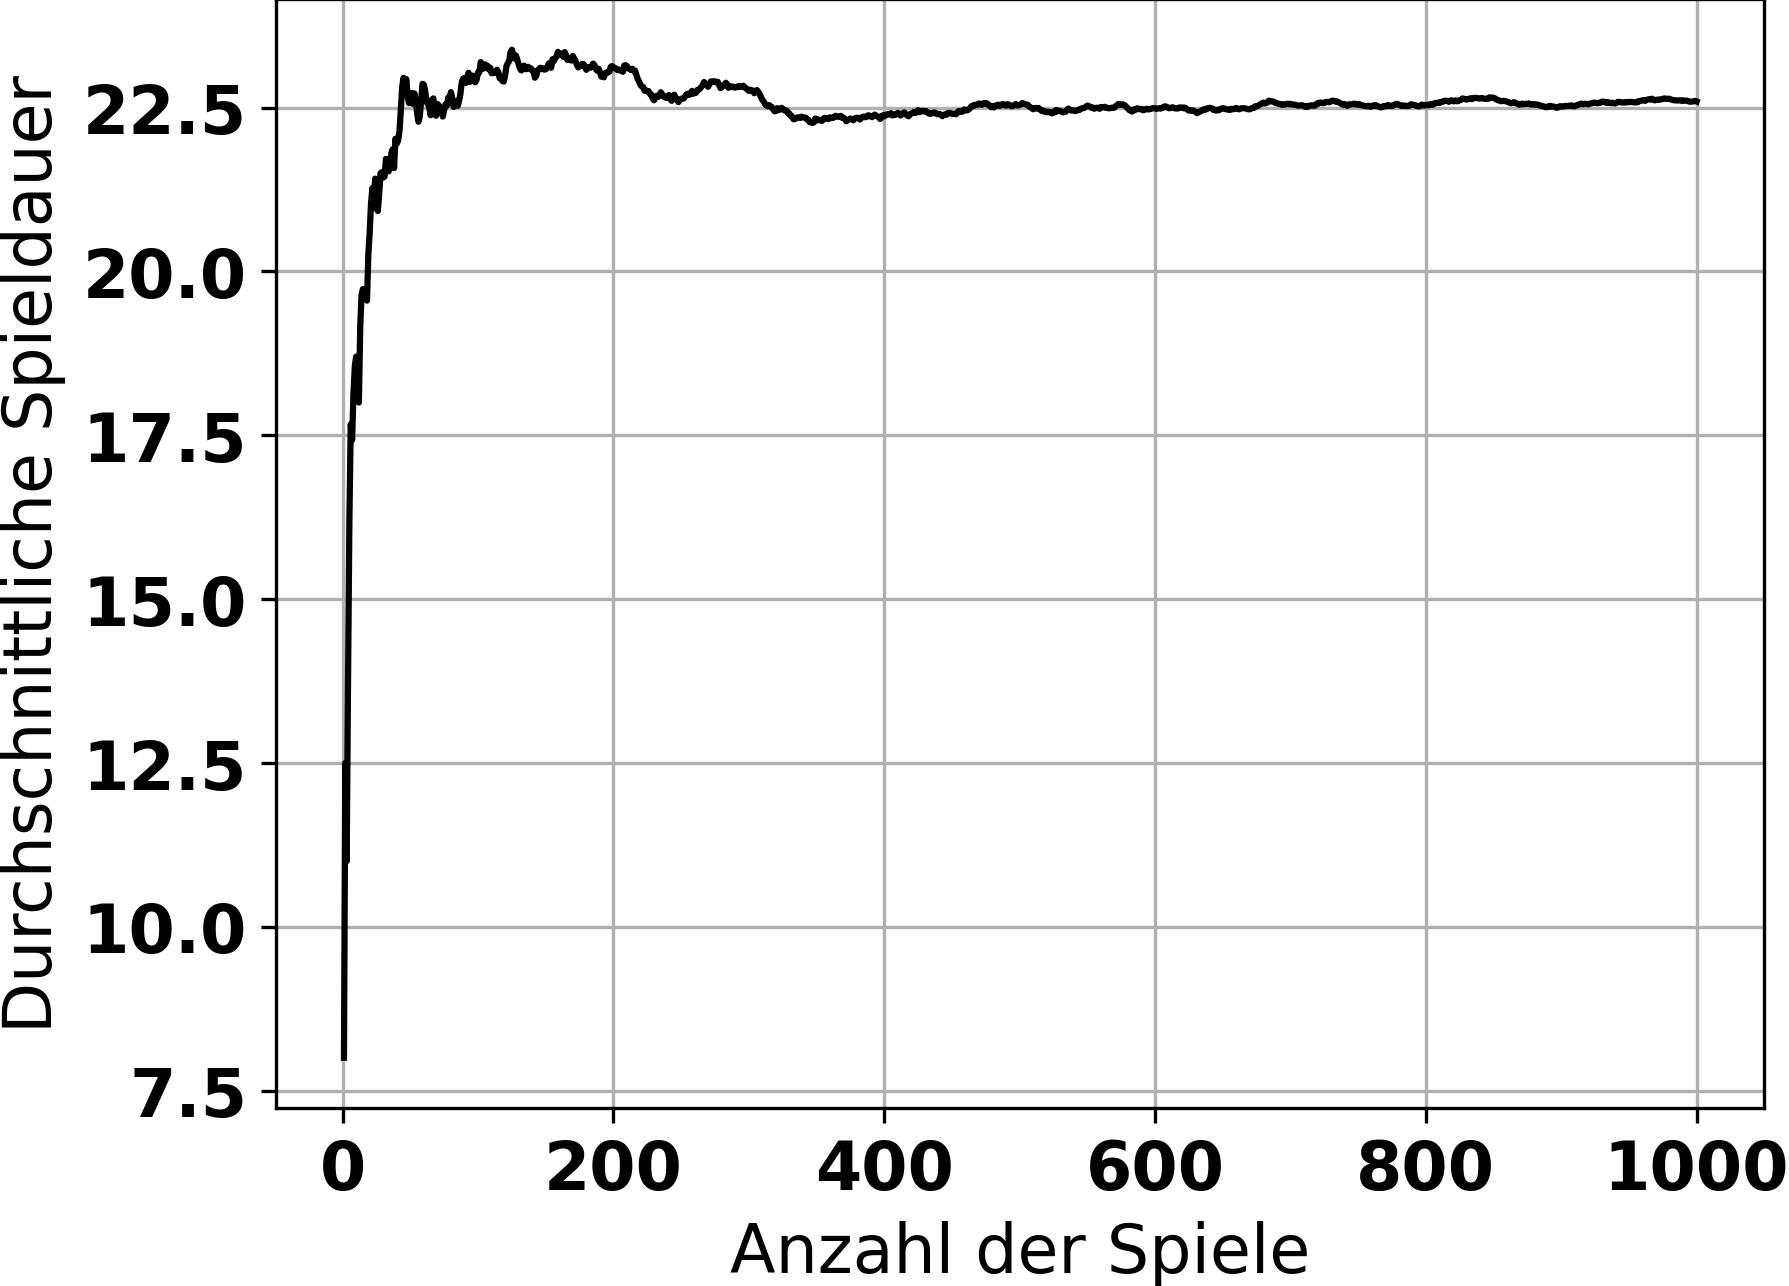
\includegraphics[width=\textwidth]{Bilder/random_vs_random_alternating_player_order_graph_game_length.png}
		\caption{Durchschnittliche Spieldauer.}
		\label{fig:f4}
	\end{subfigure}
	\caption{Gewinnrate und durchschnittliche Spieldauer bei abwechselnder Spielerreihenfolge.}
\end{figure}



\subsection{MCTS-Agent}

Bei der Implementierung des MCTS-Agenten, diente \glqq Deep Learning and the Game of Go\grqq{} (\cite{Ferguson.January2019}, Kapitel 4.5) als Orientierung. Wie im genannten Werk besteht die im Rahmen dieser Arbeit entstandenen Implementierung aus zwei Klassen. Einer Klasse \texttt{MctsNode}, die einen Knoten im MCTS-Baum abbildet, und einer weiteren Klasse \texttt{MctsAgent}, die den Agenten repräsentiert und die wesentliche Logik des Algorithmus beinhaltet.

Die Klasse \texttt{MctsNode} besitzt dabei unter anderem folgende Attribute:
\begin{itemize}
\item \texttt{parent: MctsNode} und \texttt{children: list[MctsNode]}: Sie verwalten Beziehungen zu anderen Instanzen der Klasse \texttt{MctsNode}, sodass sie zusammen den MCTS-Baum abbilden.
\item \texttt{visitation\char`_count: int }, \texttt{player\char`_0\char`_wins: int}, und \texttt{player\char`_1\char`_wins: int}: Diese Werte werden zur Berechnung der UCT-Werte in der Selection-Phase benötigt und in der Backpropagation-Phase aktualisiert.
\item \texttt{state: numpy.ndarray(6, 7, 2)}: Dabei handelt es sich um den Spielfeldzustand, den der Knoten repräsentiert. Das Format ist dabei dasselbe wie das, mit dem PettingZoo Beobachtungen über das Spielfeld zur Verfügung stellt. Dieses Attribut dient als Ausgangspunkt für die zufälligen Simulationen.
\end{itemize}

Die zentrale Methode der Klasse \texttt{MctsAgent} ist die Methode \texttt{determine\char`_action(self, state: numpy.ndarray(6, 7, 2)) -> int}. Sie nimmt den Zustand des Spielfelds entgegen, führt den MCTS-Algorithmus durch und gibt eine Zahl zurück, die die Aktion widerspiegelt, die auf Grundlage des Algorithmus gewählt werden soll. Zunächst wird darin ein Objekt der Klasse \texttt{MctsNode} initialisiert, dessen \texttt{state}-Attribut der beobachtete Zustand \texttt{state} zugewiesen wird. Dieses Objekt stellt den Wurzelknoten des MCTS-Baums dar. Anschließend werden $n$ mal folgende Methoden wiederholt, wobei $n$ die Anzahl der pro Entscheidung durchzuführenden Simulationen ist, die über den Konstruktor der Klasse konfiguriert werden kann:

\begin{itemize}
\item \texttt{select(root\char`_node: MctsNode) -> MctsNode}: Vom zuvor definierten Wurzelknoten werden per UCT-Formel solange Kinder ausgewählt, bis ein Knoten erreicht wurde, der ein Endzustand ist oder nicht vollständig expandiert ist, also weniger Kindknoten als Aktionen hat, die von dem dem Knoten entsprechenden Zustand möglich sind. Die UCT-Konstante kann dabei über den Konstruktor konfiguriert werden. Wenn es sich bei dem erreichten Knoten um einen Endzustand handelt, wird dieser Knoten zurückgegeben. Ansonsten, wird von diesem Knoten ein zufälliger legaler Spielzug ausgeführt und ein neuer Knoten, der den dadurch erreichten Zustand abbildet, wird als Kindknoten hinzugefügt. Dies entspricht dem Expansion-Schritt des MCTS-Algorithmus. Zurückgegeben wird dann der neu hinzugefügte Knoten.

\begingroup
\emergencystretch=5em
\item \texttt{simulate(selected\char`_node: MctsNode) -> str | None}: Diese Methode nimmt den in der \texttt{select}-Methode ausgewählten Knoten entgegen, das Spiel wird ab dem Zustand, den der Knoten repräsentiert, zu Ende gespielt, und zurückgegeben wird der Gewinner, bzw. None, wenn das Spiel nicht entschieden werden konnte.
\item \texttt{backpropagate(selected\char`_node: MctsNode, winner: str | None) -> None}: Von ausgewählten Knoten wird das Attribut \texttt{visitation\char`_count} erhöht und ggf. wird \texttt{player\char`_0\char`_wins} oder \texttt{player\char`_1\char`_wins} hochgezählt. Dieser Vorgang wird jeweils für alle Elternknoten durchgeführt, bis der Wurzelknoten erreicht wurde.

\endgroup
\end{itemize}

Nach n Wiederholungen wird eine Zahl zurückgegeben, die die Aktion repräsentiert, die vom Wurzelknoten zum direkten Kindknoten führt, dessen \texttt{visitation\char`_count}-At\-tribut den höchsten Wert hat.

% Anpassungen an der PettingZoo Umgebung

Für den Algorithmus wird ein Abbild für die Dynamik des Spiels benötigt, das unter anderem die Spielregeln, Gewinnbedingungen oder mögliche Aktionen in Abhängigkeit des aktuellen Zustands enthält. Dafür kommt in dieser Implementierung die Vier-Gewinnt-Umgebung von PettingZoo zum Einsatz, wodurch Aufwand in der Implementierung gespart wird. Es hat sich herausgestellt, dass an der Umgebung zwei Modifikationen notwendig sind, da die PettingZoo-Umgebungen in erster Linie zum Training von RL-Agenten konzipiert sind, und nicht um als Modell für symbolische Algorithmen oder modellbasierte RL-Verfahren zu dienen.

Zunächst wird keine Funktionalität unterstützt, um eine PettingZoo-Umgebung mit einem bestimmten Zustand zu initialisieren, was jedoch in der Klasse \texttt{MctsAgent} beispielsweise vor der Durchführung von Simulationen notwendig ist. Die Methode \texttt{reset(…, options: dict) -> None} der Vier-Gewinnt-Umgebung wurde daher erweitert, um im \texttt{options}-Parameter nach dem Schlüssel \texttt{``state''} zu suchen, unter dem der gewünschte Zustand abgelegt werden kann, und ggf. entsprechend verarbeitet wird. Der Zustand wird dabei in derselben Form erwartet, wie PettingZoo seine Beobachtungen liefert.

Eine weitere Herausforderung bestand darin, dass PettingZoo-Umgebungen Beobachtungen stets perspektivisch aus Sicht des Agenten liefern, der aktuell am Zug ist. Im Fall von Vier Gewinnt bestehen die Beobachtungen aus einem Array, das das Spielfeld repräsentiert. Dieses Array enthält sechs weitere Arrays, die jeweils eine Reihe des Spielfelds abbilden, wobei jedes dieser Arrays sieben Felder enthält, die einem Feld in der jeweiligen Reihe entsprechen. Jedes dieser Felder ist ein Array bestehend aus zwei Elementen, die jeweils die Werte 0 und 1 annehmen können. Wenn das erste Element 1 ist, bedeutet das, dass der Spieler, der aktuell am Zug ist, einen Stein an der entsprechenden Position platziert hat. Wenn das zweite Feld 1 ist, bedeutet das, dass der Gegenspieler einen Stein platziert hat. 0 bedeutet, dass der entsprechende Spieler an der Position keinen Stein platziert hat \cite{Farama.2025}. Diese perspektivischen Beobachtungen erleichtern die Implementierung von RL-Agenten. Da die Vier-Gewinnt-Umgebung von PettingZoo jedoch nicht mit perspektivischen Beobachtungen, sondern mit einem globalen Zustand arbeitet, mussten Mechanismen implementiert werden, um diesen aus den perspektivischen Beobachtungen zu erzeugen. Dazu speichert die Klasse \texttt{MctsNode}, welcher Spieler als Nächstes am Zug ist, und die Methode der Umgebung \texttt{reset(…, options: dict)} berücksichtigt einen entsprechenden Schlüssel im options-Parameter.

Aufgrund der zeitlichen Beschränkung dieser Arbeit wird auf Experimente bezüglich Optimierungen verzichtet. Daher wird als Auswahlstrategie in der Selection-Phase nach den Empfehlungen UCT mit $c=\sqrt{2}$ eingesetzt. Was die Expansion-Phase betrifft, wird sich ebenfalls an den Standard gehalten und nur einen und nicht mehrere Knoten hinzugefügt. In der Simulation-Phase werden Light-Playouts und keine Heavy-Playouts eingesetzt, da Light-Playouts ohne Wissen über das konkret zu lösende Problem auskommen, sodass die Ergebnisse dieser Arbeit so weit möglich auf verschiedene Probleme angewandt werden können.

\subsubsection{Zeitlicher Aufwand von Entscheidungen des MCTS-Agenten}

Die in dieser Arbeit durchgeführten Messungen fanden auf einem Computer mit einer Intel Core i7 8650U CPU statt. Ein MCTS-Agent, der pro Entscheidung 5.000 Simulationen durchführt, benötigt dabei für jeden Zug etwa eine zehn Sekunden. In einem Spiel mit einer Länge von 20 Zügen rechnet der MCTS-Agent damit 200 Sekunden. Für 200 Spiele, die im Rahmen dieser zeitlich begrenzten Arbeit an vielen Stellen als ausreichend für aussagekräftige Messungen betrachtet werden, werden für jeden beteiligten MCTS-Agenten mehr als elf Stunden benötigt. Die Rechenzeit verhält sich proportional zur Anzahl der durchgeführten Simulationen.

Es liegt nahe, den MCTS-Agenten durch Parallelisierung zu beschleunigen. Dadurch lässt sich die Rechenzeit proportional (ggf. sogar überproportional) zur auf der Maschine verfügbaren CPU-Ressourcen verkürzen, ohne dass die Ergebnisse dadurch beeinträchtigt werden (vgl. \cite{Chaslot.2008}). Dies ist vor allem bei Echtzeitanwendungen sinnvoll. Ein solcher Anspruch wird in dieser Arbeit jedoch nicht gestellt. Um die Komplexität des Algorithmus möglichst niedrig zu halten, wird auf die Parallelisierung von MCTS verzichtet. Stattdessen werden die Messungen parallelisiert und die Ergebnisse zusammengeführt. Wenn keine andere andere Aussage darüber getroffen wird, ist der MCTS-Agent im Rahmen dieser Arbeit so konfiguriert, dass 5000 Simulationen pro Entscheidungen durchgeführt werden.

\subsubsection{Quantitative Untersuchung}

Um einen Eindruck davon zu bekommen, von der Strategie des implementierten MCTS-Agenten in Abhängigkeit von der Anzahl der für jede Entscheidung durchgeführten Simulationen zu bekommen, wurde eine qualitative Analyse des MCTS-Agenten durchgeführt, in der 200 Spiele gegen einen zufällig spielenden Agenten mit abwechselndem Anzugsrecht durchgeführt wurden und 200 Spiele gegen sich selbst mit konstantem Anzugsrecht. Diese Messungen wurden mit 50, 100, 250, 500, 750, 1000, 2500 und 5000 Simulationen pro Entscheidung durchgeführt.

\begin{figure}[ht!]%[!tbp]
	\begin{subfigure}[b]{0.48\textwidth}
		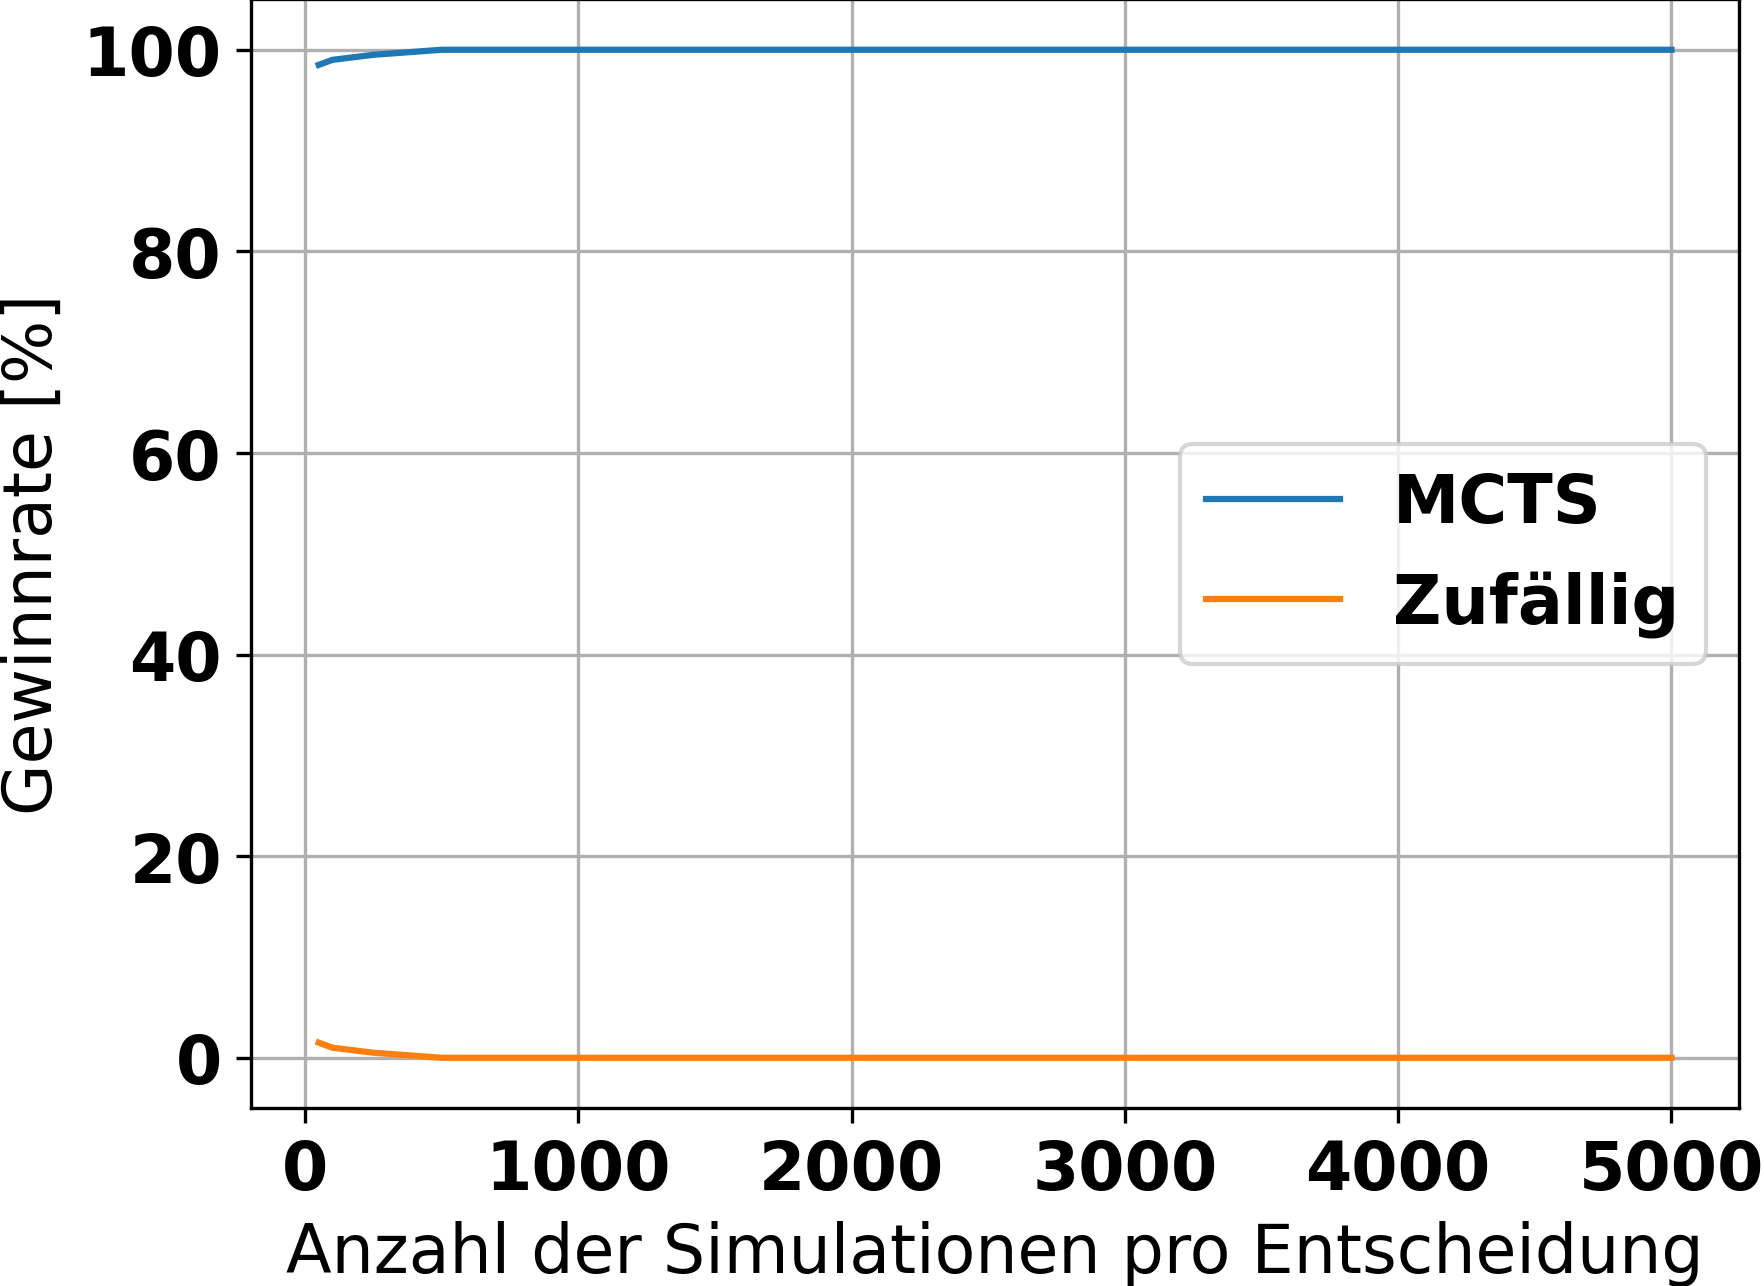
\includegraphics[width=\textwidth]{Bilder/mcts_vs_random_win_rate_vs_n_simulations.png}
		\caption{Gewinnrate.}
		\label{fig:f5}
	\end{subfigure}
	\hfill
	\begin{subfigure}[b]{0.48\textwidth}
		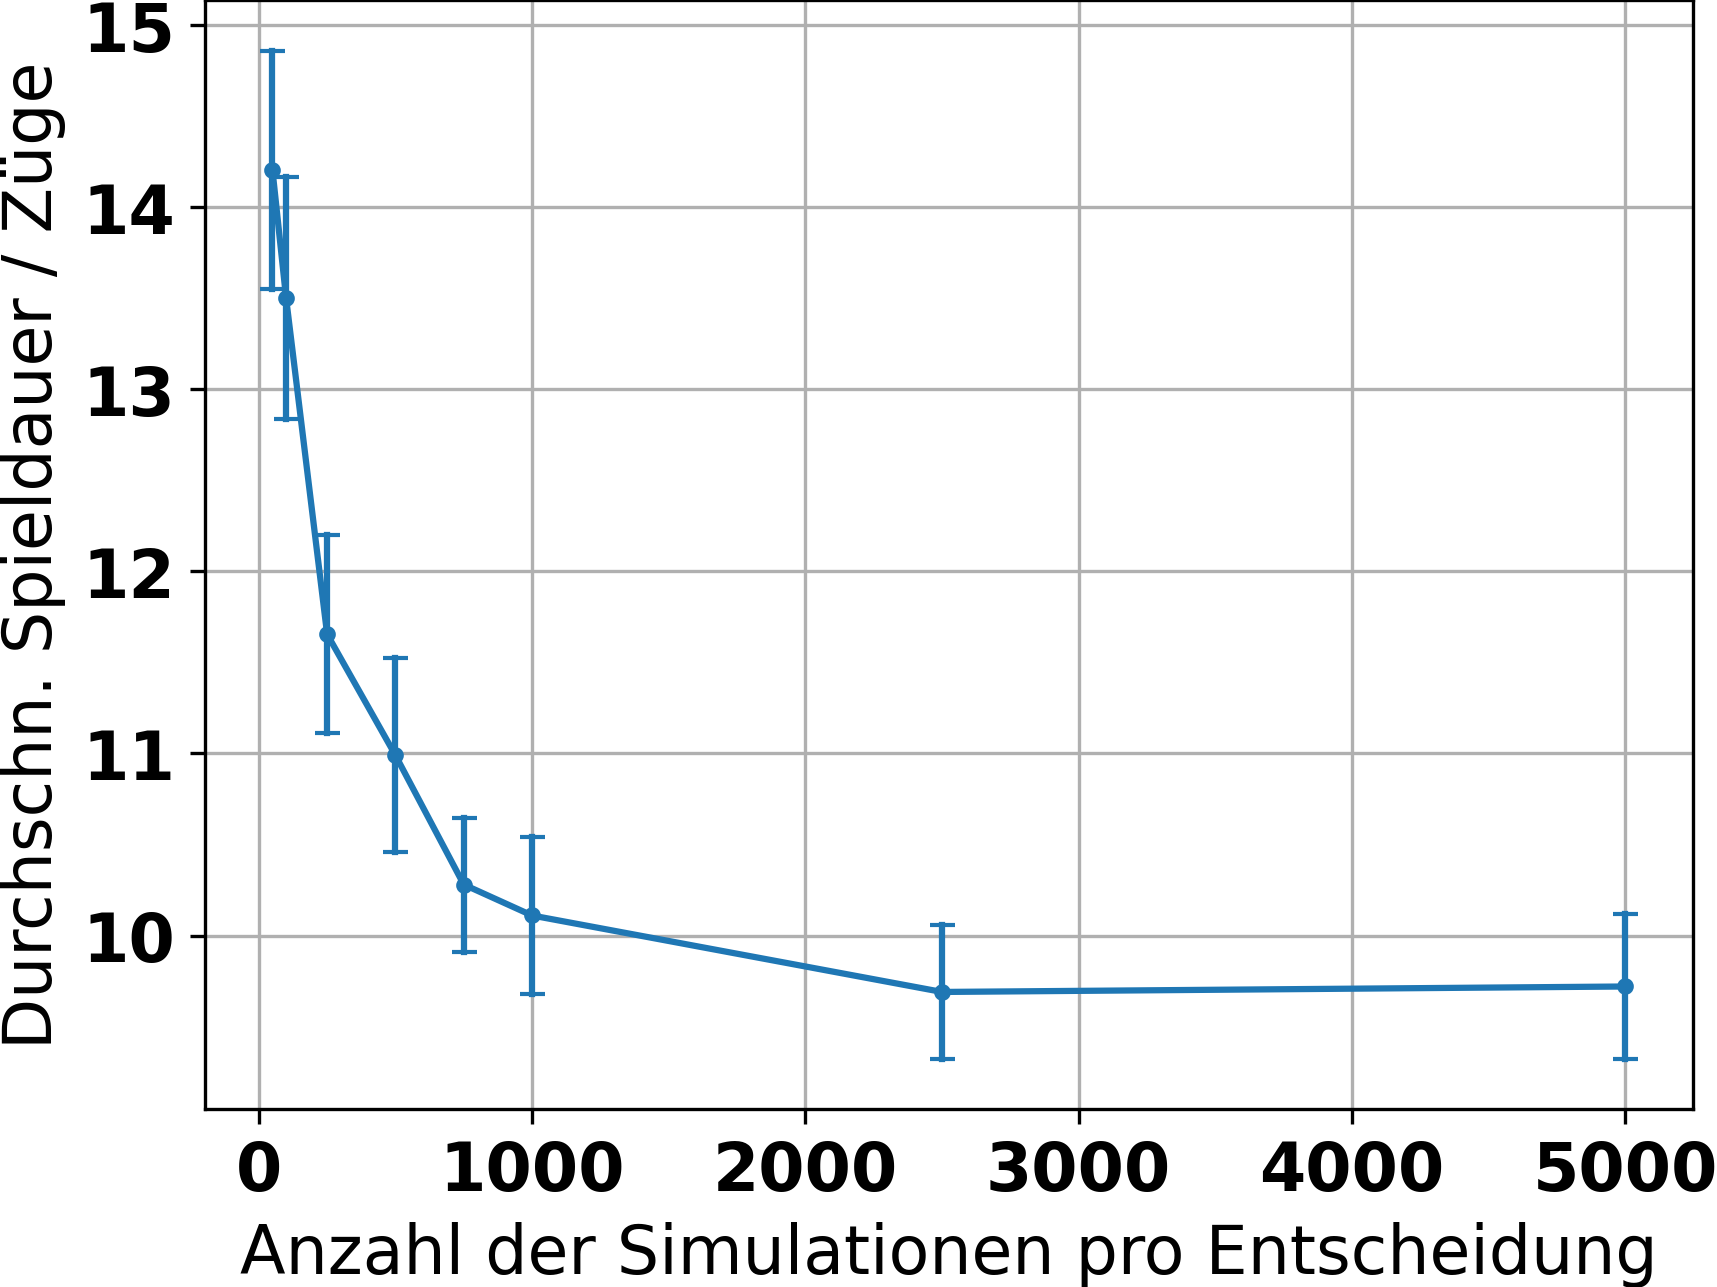
\includegraphics[width=\textwidth]{Bilder/mcts_vs_random_game_length_vs_n_simulations.png}
		\caption{Durchschnittliche Spieldauer.}
		\label{fig:f6}
	\end{subfigure}
	\caption{Gewinnrate und durchschnittliche Spieldauer in Abhängigkeit von der Anzahl der Simulationen pro Entscheidung beim Spiel eines MCTS-Agenten gegen einen zufällig spielenden Agenten.}
\end{figure}

Die Gewinnrate, die der MCTS-Agent gegen den zufällig spielenden Agenten erzielt, beträgt bei 50 Simulationen pro Entscheidung bereits 98,5 \% (95 \%-CI: 95,7 - 99,5) und steigt bis 1000 Simulationen auf 100 \% (95 \%-CI: 98,1 - 100,0), welche der Agent auch bei 2500 und 5000 Simulationen hält. Die mittlere Spieldauer startet bei 50 Simulationen mit 14.21 Zügen (95 \%-CI: 13,55 - 14,86) und flacht bei 2500 Simulationen mit 9,69 Zügen (95 \%-CI: 9,32 - 10,06) ab. Bei dem leichten Anstieg der Spieldauer bei 5000 Simulationen auf 9,72 Züge (95 \%-CI: 9,32 - 10,12) steigt, liegt durch die starke Überschneidung der Konfidenzintervalle eine stochastisch bedingte Messungenauigkeit nahe. Die kürzeste mögliche durchschnittliche Spieldauer beträgt 7.5 Züge, denn damit der anziehende Spieler gewinnt kann, müssen mindestens sieben Steine platziert sein, bzw. acht Steine, damit der nachziehende Spieler gewinnen kann. Sie ist auch bei perfekter Spielweise des MCTS-Agenten schwer zu erreichen, da ein Spiel länger dauert, sobald sein Gegenspieler eine durch den MCTS-Agenten gebildete Kette blockiert. Aus den Messungen geht hervor, dass der MCTS-Agent einem zufällig spielenden Agenten bereits bei 50 Simulationen pro Entscheidung weit überlegen ist. Auch wenn die Gewinnrate ab 1000 Simulationen 100 \% beträgt, kann über die kürzer werdende Spieldauer eine Steigerung der Leistung beobachtet werden. Der MCTS-Agent entscheidet mit steigender Anzahl von Simulationen pro Entscheidung das Spiel schneller für sich.

\begin{figure}[ht!]%[!tbp]
	\begin{subfigure}[b]{0.48\textwidth}
		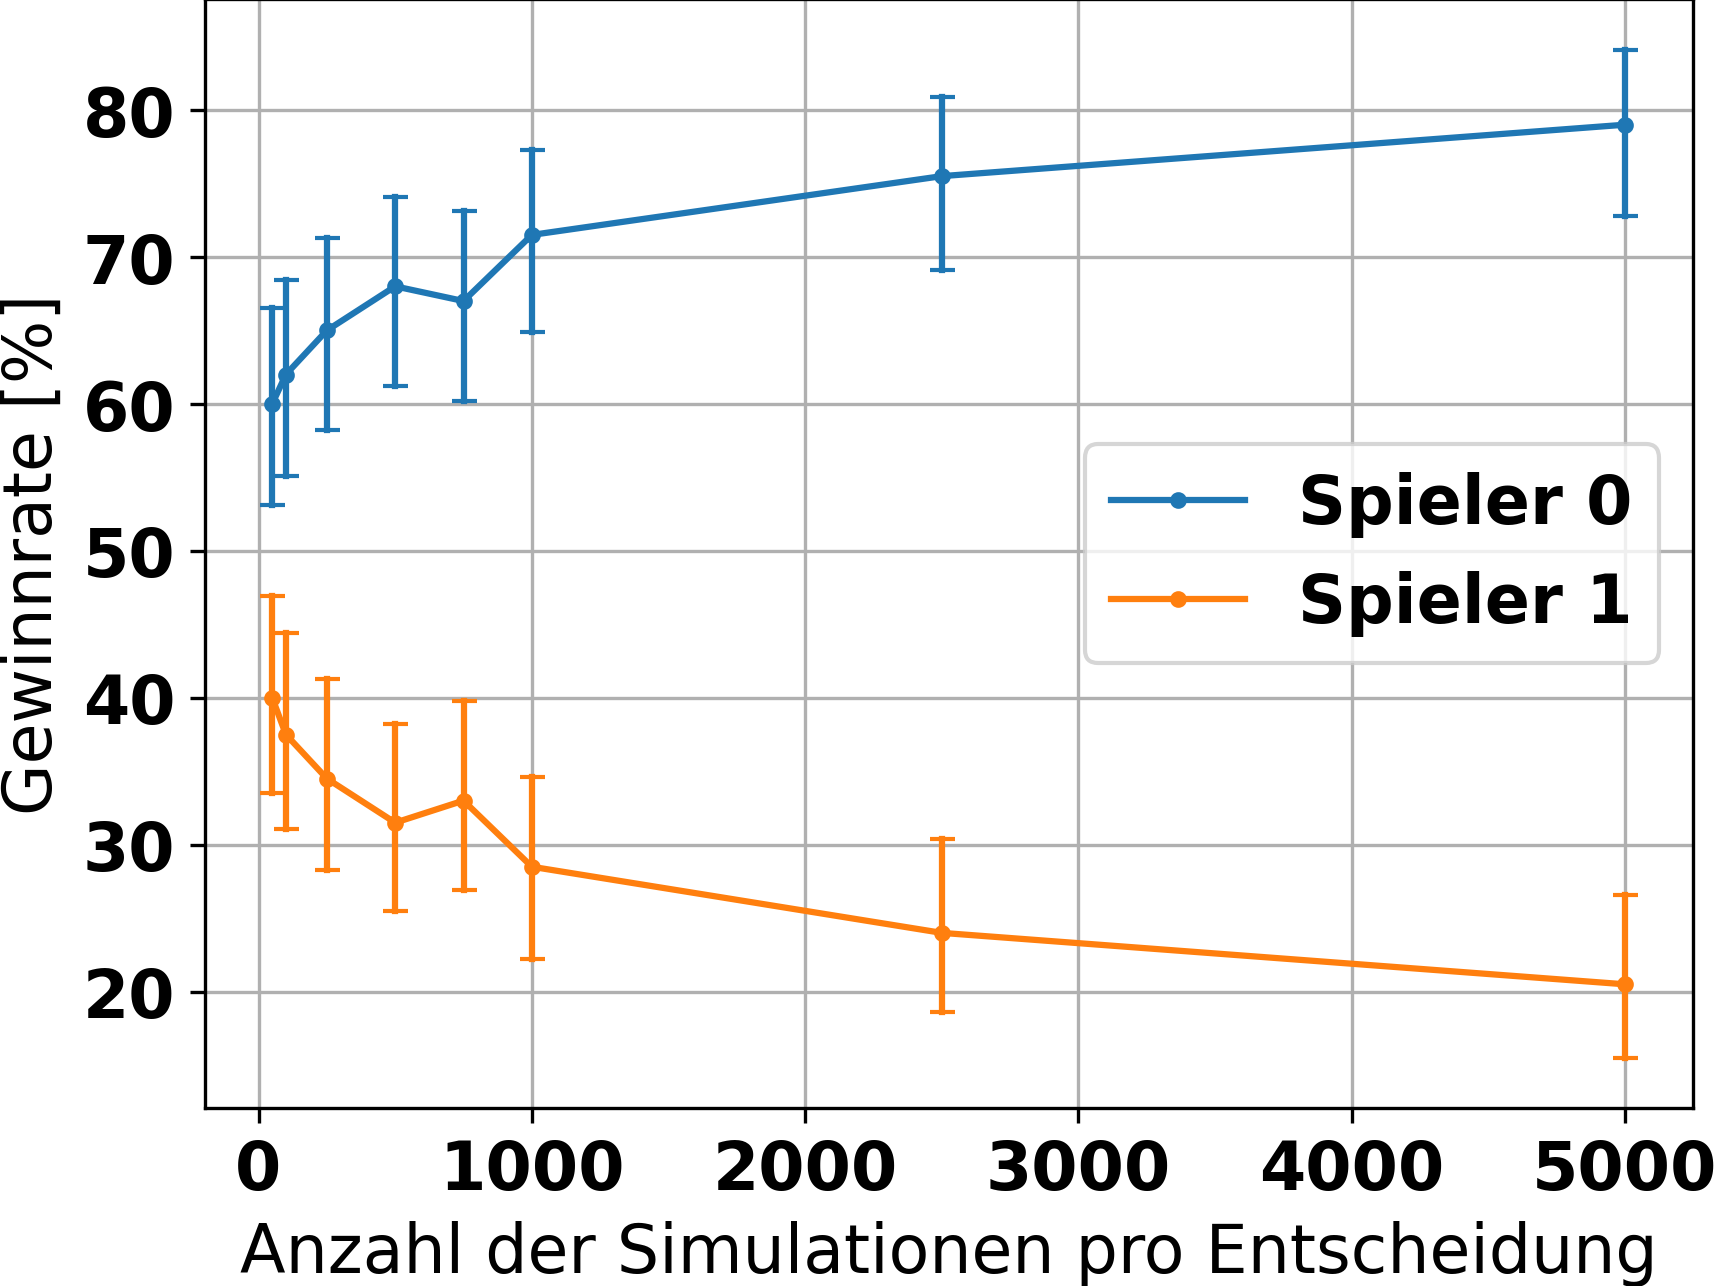
\includegraphics[width=\textwidth]{Bilder/mcts_vs_mcts_win_rate_vs_n_simulations.png}
		\caption{Gewinnrate.}
		\label{fig:f7}
	\end{subfigure}
	\hfill
	\begin{subfigure}[b]{0.48\textwidth}
		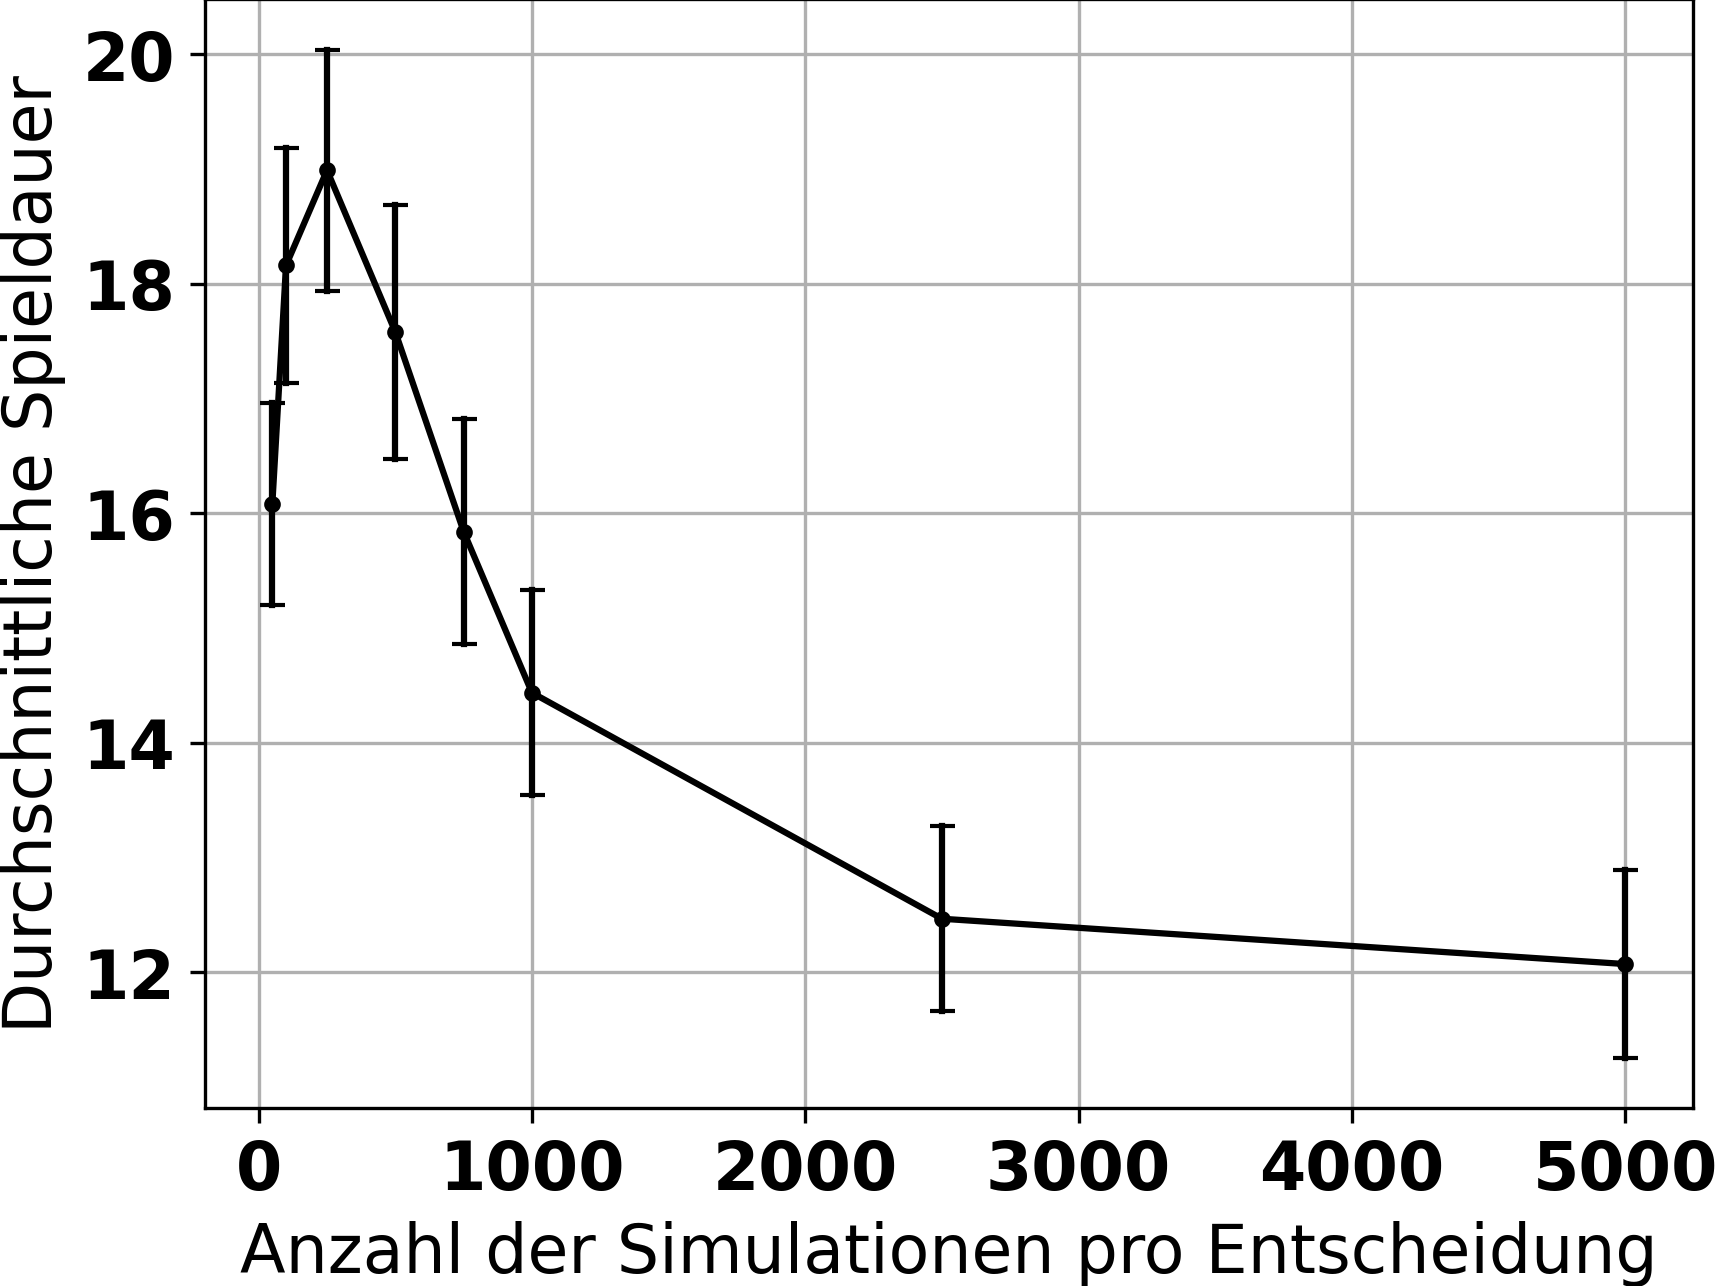
\includegraphics[width=\textwidth]{Bilder/mcts_vs_mcts_game_length_vs_n_simulations.png}
		\caption{Durchschnittliche Spieldauer.}
		\label{fig:f8}
	\end{subfigure}
	\caption{Gewinnrate und durchschnittliche Spieldauer in Abhängigkeit von der Anzahl der Simulationen pro Entscheidung beim Spiel von zwei MCTS-Agenten gegeneinander.}
\end{figure}

Spielen zwei MCTS-Agenten mit konstantem Anzugsrecht gegeneinander, hat von 50 bis 250 durchgeführten Simulationen pro Entscheidung Spieler 0 mit Gewinnraten zwischen 63,0 \% (95 \%-CI: 56,1 - 69,4) und 58,5 \% (95 \%-CI: 51,6 - 65,1) einen signifikanten Vorteil gegenüber seines Gegenspielers, was bedeutet, dass der Vorteil, das Anzugsrecht zu besitzen, ausgenutzt werden kann. Ab 500 Simulationen liegen die Messwerte nahe bei einander und die Konfidenzintervalle sind so groß, dass aus den Messungen nicht hervorgeht, ob einer der beiden Spieler signifikant einen signifikanten Vorteil hat. Bei 750 Simulationen wurden mit 50,0 \% (95 \%-CI: 43,1 - 56,9) für Spieler 0 und 49,0 \% (95 \%-CI: 42,2 - 55,9) für Spieler 1 nahezu identische Werte gemessen. Bei 5000 Simulationen wurde sogar eine mit 48,0 \% (95 \%-CI: 41,2 - 54,9) niedrigere Gewinnrate für Spieler 0 als Spieler 1 mit 52,0 \% (95 \%-CI: 45,1 - 55,8) aufgezeichnet. Aus den Konfidenzintervallen geht jedoch nicht hervor, dass sich die tatsächlichen Werte auch so verhalten.

Dieser Verlauf in der Hinsicht überraschend, als dass der MCTS-Algorithmus bei Vier Gewinnt mit steigender Simulationsanzahl zu perfektem Spielverhalten konvergieren sollte, wodurch der anziehende Spieler mit zunehmender Anzahl von durchgeführten Simulationen mehr Spiele für sich entscheiden sollte. Eine Erklärung dafür bei den durchgeführten Messungen, ein solches Verhalten nicht beobachtet wird, ist dass dafür der MCTS-Agent auch mit 5000 Simulationen pro Entscheidung vom perfekten Spielverhalten noch zu weit entfernt ist. Bis 5000 Simulationen erhöht sich die Fähigkeit des MCTS-Agenten zu verteidigen schneller als seine Fähigkeit anzugreifen, wodurch beide Spieler jeweils etwa die Hälfte der Spiele gewinnen.

Die mittlere Spieldauer steigt von 50 Simulationen bis 750 Simulationen stetig von 18,19 (95 \%-CI: 17,11 - 19,27) auf 32,11 \% (95 \%-CI: 31,10 - 33,03). Der Verlauf flacht dabei ab, sodass für die darauf folgenden Werte keine Aussagen darüber getroffen werden können, ob sie weiterhin steigen oder nicht. Die zunächst steigende Spieldauer deutet darauf hin, dass die MCTS-Agenten längerfristige Strategien entwickeln, sodass komplexere Spielsituationen zustande kommen.

\subsubsection{Qualitative Untersuchung}

\label{qualitative-untersuchung}

Neben der quantitativen Analyse gegen zufällig spielende Agenten und gegen sich selbst wurde auch eine kurze qualitative Analyse im Spiel gegen einen menschlichen Spieler durchgeführt, um einen Eindruck über das strategische Spielverhalten des MCTS-Agenten zu gewinnen, das aus den quantitativen Analysen nicht hervorgeht. Der menschliche Spieler ist bei den Untersuchungen stets der Spieler, der den ersten Stein setzen darf. Er kann damit theoretisch jedes Spiel gewinnen und hat so mehr Kontrolle über den Spielverlauf, was die Analyse vereinfacht.

Ist der MCTS-Agent konfiguriert, um 250 Simulationen pro Entscheidung durchzuführen, lässt sich beobachten, dass bei drei bereits in einer Kette platzierten Spielsteinen, stets auch der vierten Spielstein platziert wird, um zu gewinnen, sofern dies möglich ist. Wenn hingegen durch seinen Gegenspieler drei Steine in einer Kette platziert wurden, wird durch den MCTS-Agenten häufig versäumt, den vierten Stein zu blockieren, sodass der Gegenspieler das Spiel für sich entscheiden kann. Wird der MCTS-Agent nicht unter Druck gesetzt, wirken seine Züge häufig ziellos. Wenn er Angriffe vorbereitet, sind seine Züge leicht durchschaubar, was es als Mensch recht einfach macht, sie zu verteidigen. Es ist auch ohne strategische Kenntnisse des Spiels leicht möglich, gegen den MCTS-Agenten zu gewinnen. Ein Vorgehen das dabei häufig funktioniert, besteht darin, darauf abzuzielen, einen Stein in der vierten Reihe der mittleren Spalte platziert zu bekommen, und von dort aus eine diagonale Kette nach links unten oder rechts unten zu bilden. Manchmal geht dieser Plan nicht auf, jedoch entwickeln sich dadurch im Laufe des Spiels schnell andere offensichtliche Gewinnchancen.

Bei 1.000 Simulationen pro Entscheidung wird durch den MCTS-Agenten sein erster Stein meistens im untersten Feld der mittleren Spalte platziert, sofern es frei ist, was laut Allis auch der stärkste Anfangszug ist \cite{Allis.1988}. Hat der Gegenspieler drei Steine in einer Kette positioniert, so wird diese Angriffsposition meistens durch den MCTS-Agenten verteidigt. Es macht sich auch bemerkbar, dass der Agent wesentlich aggressiver spielt. Werden durch den Gegenspieler beispielsweise seine Steine zu Beginn des Spiels so platziert, dass er keine Gefahr darstellt und die Bildung von Viererketten erst zum letztmöglichen Zeitpunkt verteidigt, baut der Agent Druck auf, sodass der Gegenspieler im restlichen Verlauf des Spiels häufig dazu gezwungen ist, einen bestimmten Zug zu wählen, um nicht im nächsten Zug zu verlieren. Verteilt der Gegenspieler seine ersten drei Steine auf die beiden gegenüberliegenden Ränder, erzeugt der Agent häufig eine Zwickmühle, in dem er seine ersten drei Steine jeweils in die unterste Reihe der drei mittleren Spalten platziert, sodass er im nächsten Zug gewinnen kann, indem er seinen Stein in der zweiten oder vorletzten Spalte platziert. Dieses Verhalten konnte bei 250 Simulationen nicht beobachtet werden. Auch hier gelingt die oben genannte Strategie, sich als Ziel zu setzen, eine Diagonale von einer unteren Ecke zur Position in der mittleren Spalte in der vierten Reihe zu bilden. Allerdings scheint der MCTS-Agent besser voraus zu planen, denn die Spiele dauern länger und sein Gegenspieler muss häufiger verteidigen.

Bei 5.000 Simulationen pro Zug wird der erste Spielstein des MCTS-Agenten, wenn möglich, stets in das unterste Feld der mittlere Spalte platziert. Es ist eine verstärkte Bildung von Zwickmühlen zu bemerken, sofern sie durch den Gegenspieler nicht frühzeitig erkannt und verhindert werden. Durch seine noch aggressivere Spielweise, ist es nur unter besonderer Anstrengung möglich, als menschlicher Spieler ohne Kenntnisse über die optimale Spielweise gegen den MCTS-Agenten zu gewinnen.

\subsection{PPO-Agent}

Die Implementierung des PPO-Agenten erfolgte im Rahmen dieser Arbeit mit Hilfe des Frameworks Stable Baselines3. Es wurde zunächst versucht, mit der Trainingsstrategie von Zhong et al. einen PPO-Agenten zu entwickeln, der mit dem MCTS-Agenten mithalten kann. Dies ist jedoch mangels zeitlicher Ressourcen nicht gelungen. Aus diesem Grund wurde auf eine einfachere Trainingsstrategie umgestellt, die darin besteht, das PPO-Modell gegen einen zufällig spielenden Agenten zu trainieren.

\subsubsection{Einführung in Stable Baselines3}

Das PPO-Verfahren wird in dieser Arbeit nicht von Grund auf implementiert. Stattdessen wird auf eine Implementierung des Verfahrens aus dem Framework Stable Baselines3 zurückgegriffen. Dieses Framework enthält Implementierungen von verschiedenen RL-Verfahren, die auf den Referenzimplementierungen von OpenAI aufbauen. Das Framework bietet eine Schnittstelle, die es ermöglicht, die implementierten RL-Verfahren auf Gymnasium-Umgebungen anzuwenden. Aufgrund der Ähnlichkeit der Schnittstellen von Gymnasium und PettingZoo lässt sich Stable Baselines3 auch auf PettingZoo-Umgebungen anwenden \cite{Raffin.2021} \cite{Farama.2025}.

Die grundlegende Vorgehensweise bei der Verwendung des Frameworks besteht darin, aus einer Klasse, die ein ausgewähltes RL-Verfahren implementiert (z.B. PPO), ein Objekt zu erzeugen, das ein zu trainierendes RL-Modell repräsentiert. Diesem Modell wird dabei eine Gymnasium- oder PettingZoo-Umgebung zugeordnet, in der das Modell trainiert werden soll. Anschließend kann das Training über die Methode des Modells \texttt{learn(total\char`_timesteps: int)} starten. Dabei beschreibt \texttt{total\char`_timesteps} die Anzahl von Schritten, die in der Trainingsumgebung durchgeführt werden sollen \cite{Raffin.2021}.

Bei jedem Schritt wird die Step-Methode des Umgebung aufgerufen, die die Aktion eines Agenten entgegen nimmt und den Zustand der Umgebung entsprechend verändert. Wurde ein Endzustand erreicht, wird die Reset-Methode der Umgebung aufgerufen, die die Umgebung wieder in den Ursprungszustand versetzt. Über optionale Funktionsparameter ist es möglich, Hyperparameter des Trainings anzupassen. Dazu gehören beispielsweise die Lernrate, die Architektur der neuronalen Netzwerke des RL-Modells, oder die Anzahl von durchzuführenden Trainingsschritten bis die Parameter der Netzwerke auf Grundlage der zuletzt gesammelten Erfahrungen aktualisiert werden sollen \cite{Raffin.2021}.

\paragraph{Wrapper}

\label{wrapper}

Wird einem Modell eine PettingZoo-Umgebung direkt zugeordnet und anschließend ein Training gestartet, so wird das Modell die Züge für alle Agenten der Umgebung durchführen und im Laufe des Trainings seine Parameter auf Grundlage der Belohnungen jedes Agenten anpassen \cite{Farama.2025}. Dadurch wird das in MARL allgegenwärtige Moving-Target-Problem verstärkt. Wenn alle Agenten der Umgebung ihre Parameter gleichzeitig aktualisieren, versucht jeder Agent, sich an das Verhalten der anderen sich ändernden Agenten anzupassen. Das kann zyklisches und instabiles Lernverhalten hervorrufen (\cite{Albrecht.2024}, S. 12). Aus diesem Grund ist es gängige Praxis bei MARL, nur einen Agenten auf einmal zu trainieren und die anderen Agenten stationär zu halten (\cite{Albrecht.2024}, S. 300; \cite{Zhong.2020}).

Um dieses Verhalten abbilden zu können, wird für die Implementierung der Trainingsstrategien die PettingZoo-Umgebung von Vier Gewinnt von einem Wrapper umschlossen, der nach außen dieselbe Schnittstelle bereitstellt, wie die Umgebung selbst. Die Vier-Gewinnt-Umgebung wird nicht direkt dem Modell zugeordnet, sondern der Wrapper, der diese Umgebung enthält. Die Step-Methode wurde über den Wrapper erweitert, nicht nur den Zug auszuführen, den das trainierende Modell gewählt hat, sondern auch den Zug, der durch ein stationäres Regelwerk gewählt wird. Damit das Modell trotzdem lernen kann, nicht nur als erster sondern auch als zweiter Spieler zu spielen, kann in der Reset-Methode Logik eingebunden werden, um einen Zug für einen stationären Agenten durchzuführen, und damit das Anzugsrecht zu wechseln.

\paragraph{Action Masking}

\begingroup
\emergencystretch=5em

Neben den bereits in Kapitel \ref{a2c} genannten Vorteilen besitzt das Verfahren PPO auch den Vorteil, dass Stable Baselines3 die Implementierung \texttt{MaskablePPO} enthält, die Action Masking unterstützt. Für A2C existiert derzeit keine solche Implementierung \cite{Raffin.2021}. Action Masking sorgt dafür, dass das Modell im Training und in der Anwendung daran gehindert wird, Entscheidungen zu treffen, die die Umgebung nicht erlaubt \cite{Huang_2022}. Im Vier Gewinnt bedeutet das beispielsweise, einen Spielstein in eine Spalte zu platzieren, in der bereits alle Felder belegt sind. Die PettingZoo-Umgebung ist zwar darauf ausgelegt, bei illegalen Aktionen das Spiel zu beenden und den verantwortlichen Agenten mit einer entsprechenden negativen Belohnung zu bestrafen \cite{Farama.2025}. Es wurde jedoch gezeigt, dass der Einsatz von Action Masking effektiver ist als sich auf die Bestrafung über die Umgebung zu verlassen \cite{Huang_2022}.

\endgroup

Damit Action Masking in der Implementierung der Trainingsumgebung funktioniert, muss die dem Modell zugeordnete Umgebung eine Methode \texttt{action\char`_mask()} implementieren, die Auskunft darüber gibt, welche Aktionen möglich und welche nicht möglich sind. Das ist in den PettingZoo-Umgebungen standardmäßig nicht der Fall. Diese Funktionalität wurde daher dem oben genannten Wrapper hinzugefügt.

\subsubsection{Implementierte Trainingsverfahren}

Im Rahmen der Arbeit wurden zwei verschiedene Trainingsverfahren implementiert. Ersteres konnte aufgrund mangelnder Zeit nicht erfolgreich umgesetzt werden. Aus diesem Grund wurde auf eine einfachere Trainingsstrategie umgestellt.

\paragraph{Verfahren nach Zhong et al.}

Zunächst wurde versucht, die in \cite{Zhong.2020} von Zhong et al. herausgearbeitete Trainingsstrategie für Zwei-Spieler-Nullsummenspiele zu implementieren. Im Zuge dieser Strategie werden mehrere Modelle auf einmal trainiert. Die Modelle sind dabei in $n$ 2-Tupel organisiert. Die jeweils ersten Modelle der Tupel spielen stets als erster Spieler und die jeweils zweiten Modelle der Tupel spielen stets als zweiter Spieler. Folgende zwei Schritte werden für $N$ Iterationen wiederholt:

\begin{itemize}
	\item Jedes erste Modell aller Tupel wird gegen jedes zweite Modell aller Tupel durch wiederholte Spiele evaluiert. Dabei werden die Gewinnraten aufgezeichnet.
	\item Anschließend werden alle Modelle für $l$ Trainingsschritte jeweils gegen das Modell trainiert, gegen das die niedrigste Gewinnrate erzielt wurde.
\end{itemize}

In der genannten Arbeit wurde für verschiedene exemplarische Anwendungsfälle gezeigt, dass diese Strategie zu leistungsfähigeren Modellen führt als andere weit verbreitete Self-Play-Strategien. Diese anderen Strategien bestehen häufig darin, ein Modell wiederholt für eine bestimmte Anzahl von Trainingsschritten gegen eine ältere und stationäre Version von sich selbst zu trainieren und zwischenzuspeichern. Bei jeder Wiederholung wird der Gegenspieler durch das neuste, beste oder ein zufälliges zwischengespeichertes Modell ersetzt.

Ein Anwendungsfall, an dem in \cite{Zhong.2020} die überlegene Leistungsfähigkeit des Verfahrens gezeigte wurde, ist die 9 x 9 Variante des Spiel Gomoku. Das Konzept des Spiels ist dabei ähnlich wie das von Vier Gewinnt. Das Spielfeld ist jedoch nicht 7 x 6, sondern 9 x 9 Felder groß, zum Gewinnen müssen fünf und nicht vier Spielsteine in einer Kette platziert werden, und die Spielsteine fallen nicht in das unterste Feld einer Spalte, sondern können auf beiden Achsen beliebig positioniert werden. Da Vier Gewinnt damit einen kleineren Zustands- und Aktionsraum besitzt, liegt nahe, dass die in \cite{Zhong.2020} vorgestellte Trainingsstrategie auch für Vier Gewinnt funktioniert.

% Anwendung auf vier Gewinnt

Im Rahmen dieser Arbeit wurde das Verfahren mit den Lernraten $\alpha_0 = 0,001$, $\alpha_1 = 0,003$ (Standardwert aus Stable Baselines3), $\alpha_2 = 0,0001$, $\alpha_3 = 0,00003$ und $\alpha_4 = 0,00001$ durchgeführt. In \cite{Zhong.2020} werden nach der Evaluation jeweils so viele Trainingsschritte durchgeführt, bis $l = 10$ Parameteraktualisierungen der RL-Modelle hervorgerufen wurden. Nach dem voreingestellten Hyperparametern der Implementierung von PPO in Stable Baselines3 werden die Parameter der neuronalen Netzwerke nach 2048 Trainingsschritten aktualisiert. Bei der Anwendung des Verfahrens in dieser Arbeit werden daher 20480 Schritte durchgeführt, um die gleiche Anzahl von $l = 10$ Parameteraktualisierungen hervorzurufen wie in \cite{Zhong.2020}. Die Anzahl der Iterationen $N$ beträgt in \cite{Zhong.2020} je nach Anwendungsfall 40 bzw. 50. Um die Wahrscheinlichkeit zu reduzieren, dass das Training aufgrund von zu kurzer Dauer fehlschlägt, wurde in dieser Arbeit $N = 100$ gewählt. Die Architektur der neuronalen Netzwerke und alle anderen Hyperparameter werden bei den Standardwerten von Stable Baselines3 belassen.

Während der Trainings mit den verschiedenen Lernraten wurde nach allen $N$ Iterationen jeweils der durchschnittliche Policy-Gradient-Verlust und Werteverlust der Iteration, und die über 500 Spiele gemittelte Gewinnrate und Spieldauer von zufälligen Modelltupeln gegen einen zufällig spielenden Agenten aufgezeichnet. Der Policy-Gradient- und Werteverlust werden jeweils als Maß dafür verwendet, wie stark die Gewichte des Actor- bzw. Ciritc-Netzwerks angepasst werden. Konvergieren die Verluste gegen Ende des Trainings in der Nähe von 0, deutet das darauf hin, dass das Modell sein Optimierungspotenzial ausgeschöpft hat und kein neues Verhalten mehr lernt. Ergänzend zu den hier präsentierten Trainingsmetriken mit ausgewählten Gewinnraten finden sich im Anhang \ref{appendix-training-zhong} zusätzliche Diagramme zu den Trainings mit allen weiteren Gewinnraten.

% Ergebnis der Anwendung auf Vier Gewinnt

\begin{figure}[ht!]%[!tbp]
	\begin{subfigure}[b]{0.48\textwidth}
		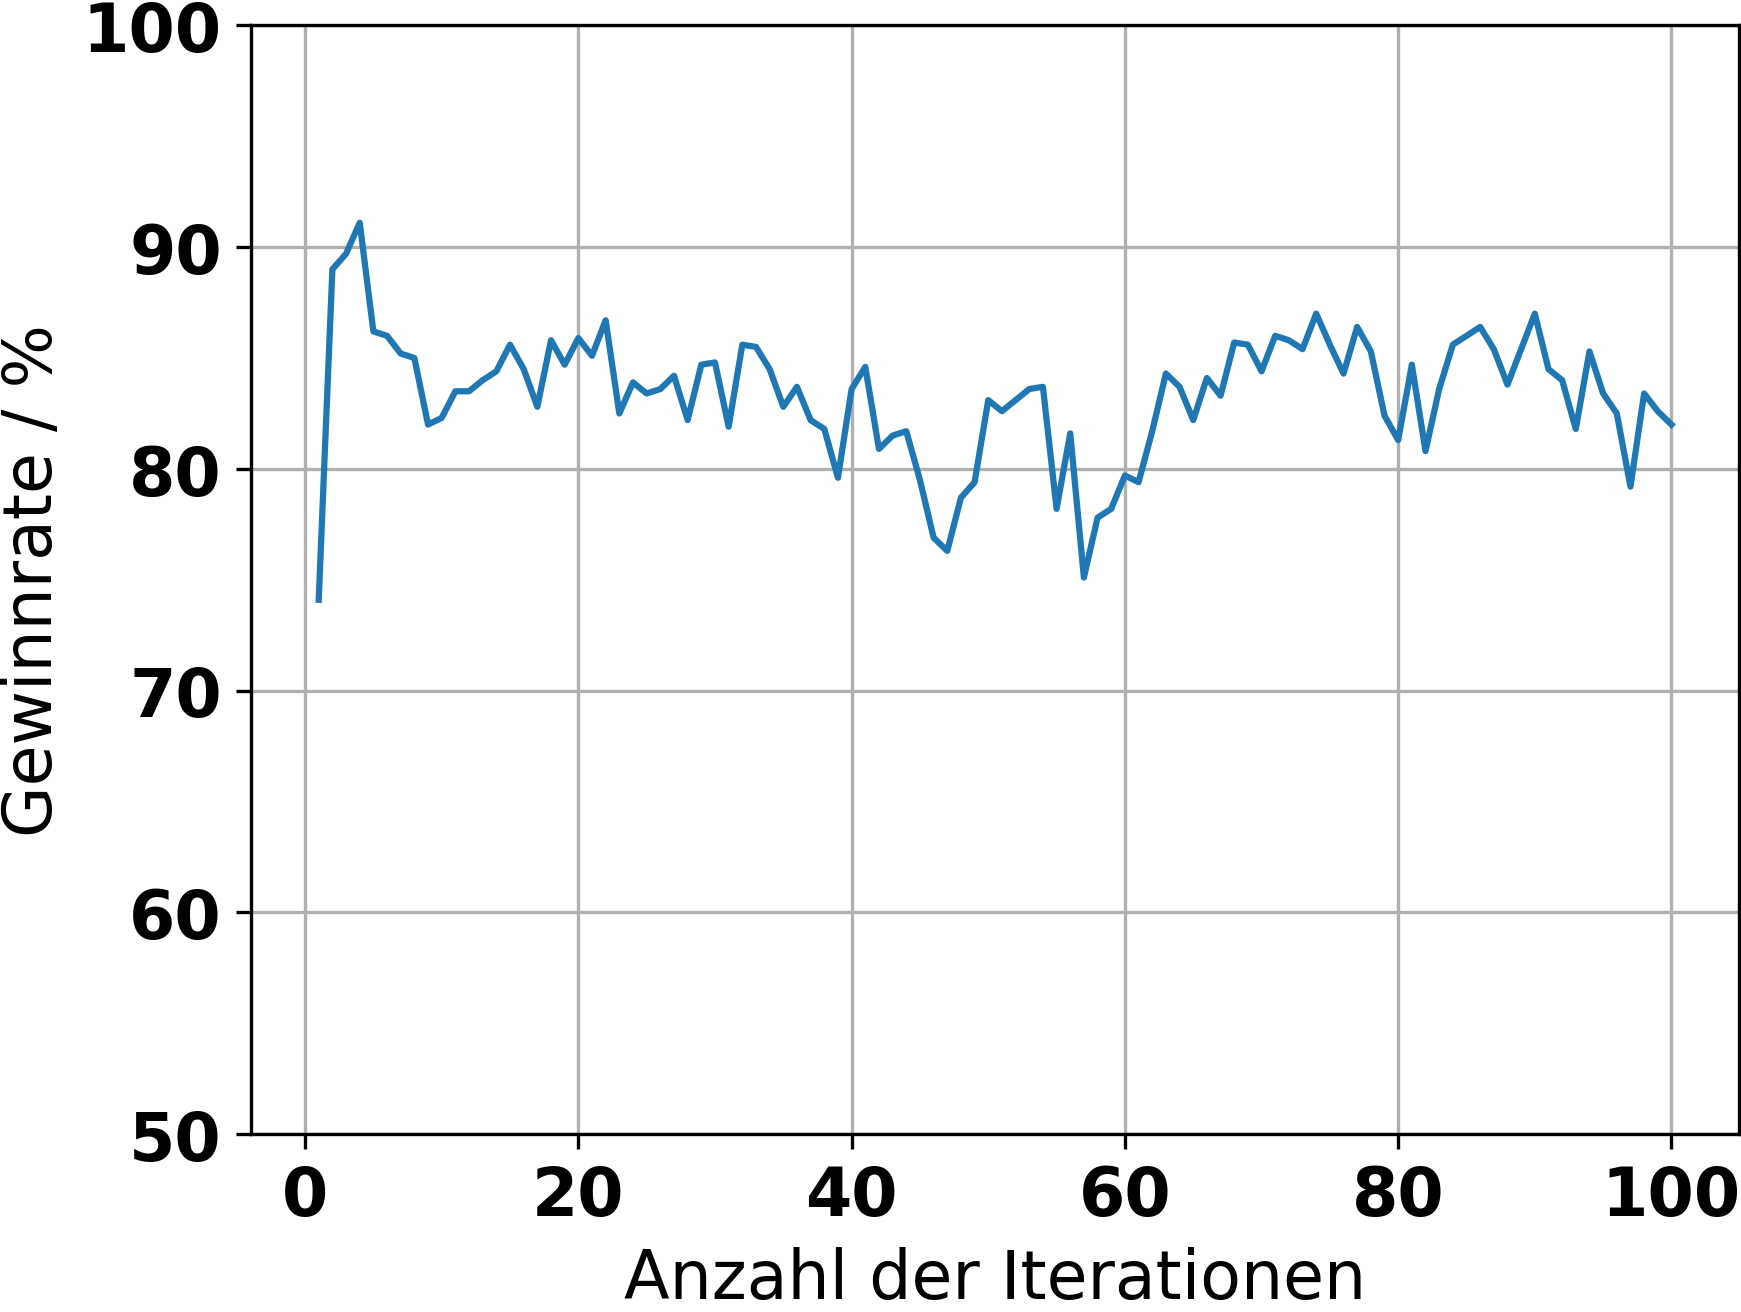
\includegraphics[width=\textwidth]{Bilder/ensemble-training/a_0_001/graph_win_rates.png}
		\caption{Verlauf der Gewinnrate mit Lernrate $\alpha_0$.}
		\label{fig:f9}
	\end{subfigure}
	\hfill
	\begin{subfigure}[b]{0.48\textwidth}
		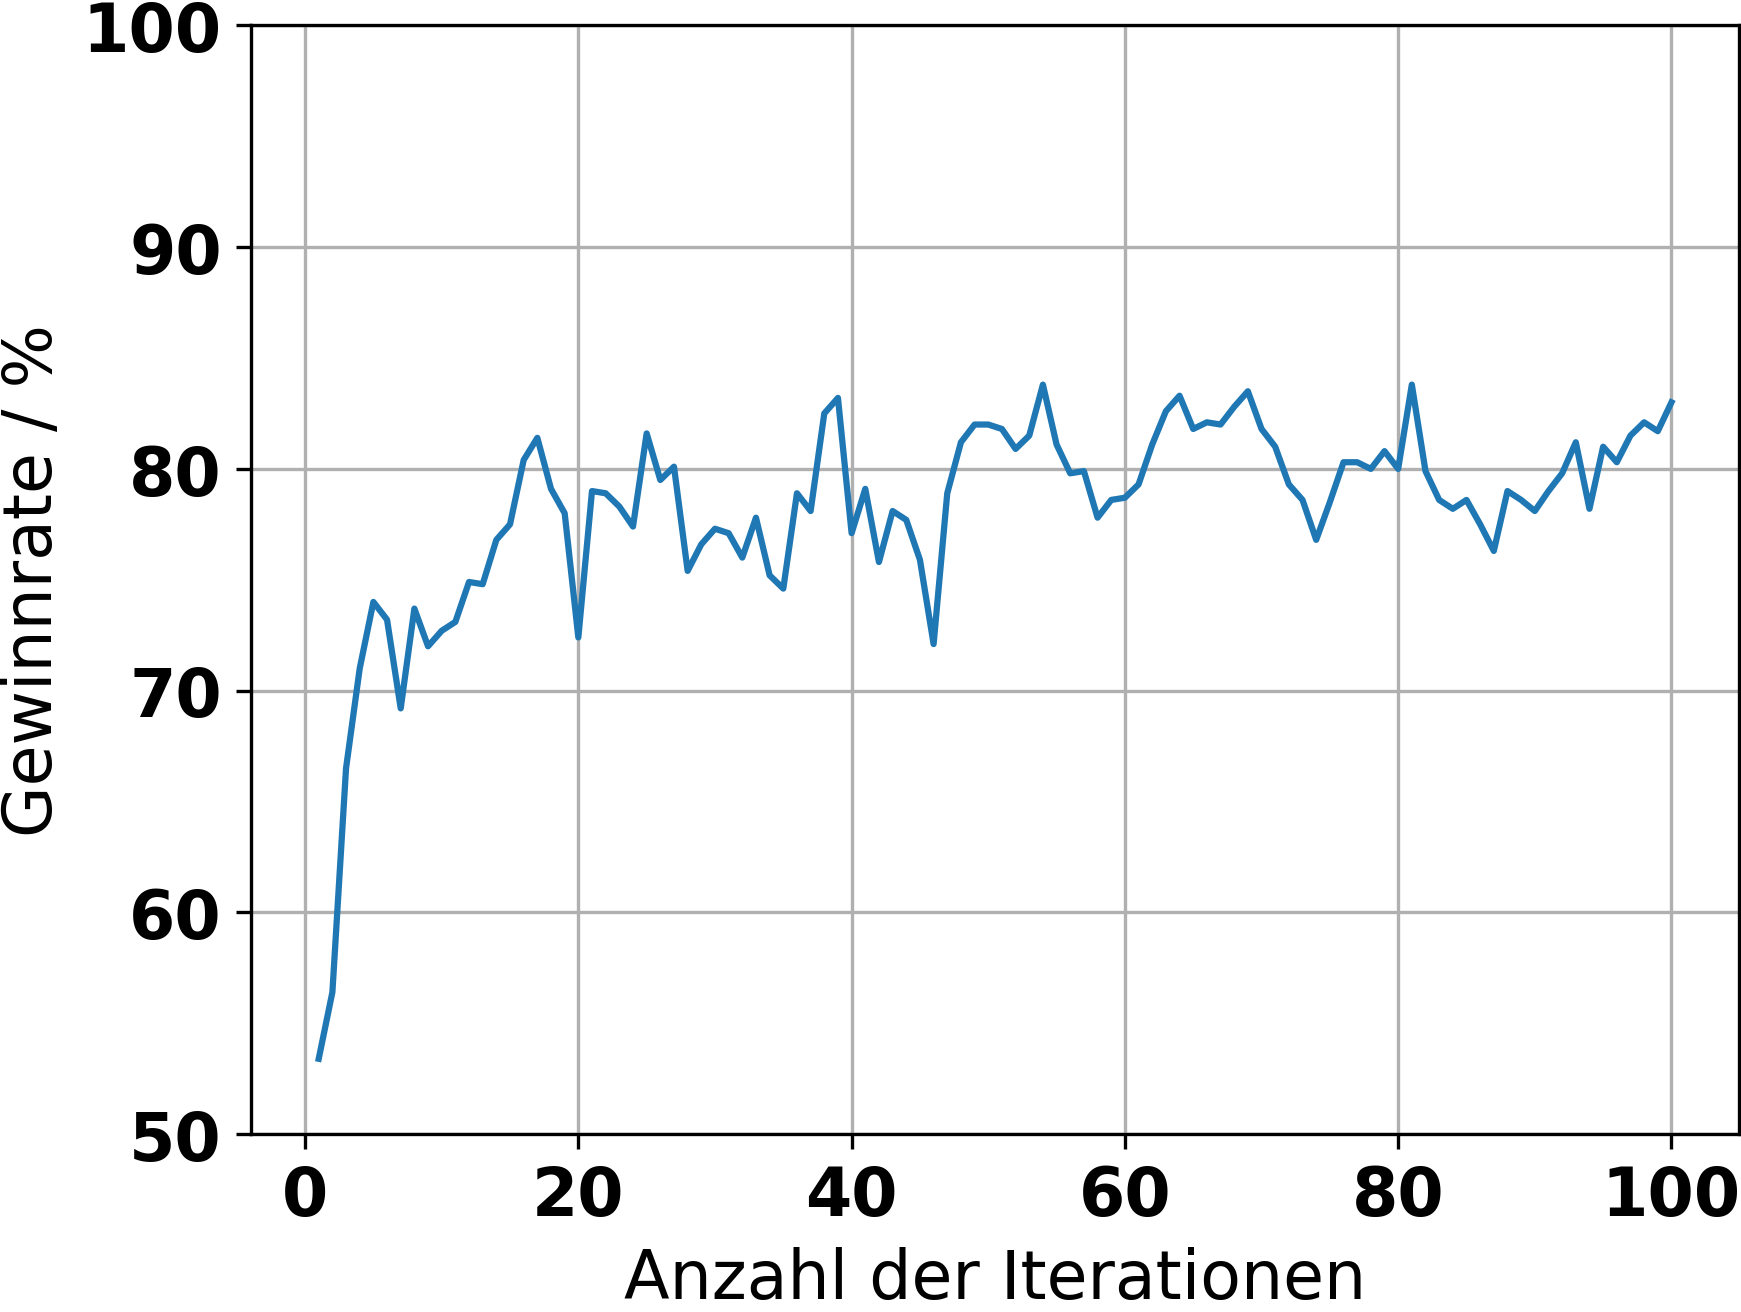
\includegraphics[width=\textwidth]{Bilder/ensemble-training/e_0_00001/graph_win_rates.png}
		\caption{Verlauf der Gewinnrate mit Lernrate $\alpha_4$.}
		\label{fig:f10}
	\end{subfigure}
	\caption{Verlauf der Gewinnrate während des Trainings nach Zhong et al. mit den Lernraten $\alpha_0$ und $\alpha_4$}
\end{figure}

\begin{figure}[ht!]%[!tbp]
	\begin{subfigure}[b]{0.48\textwidth}
		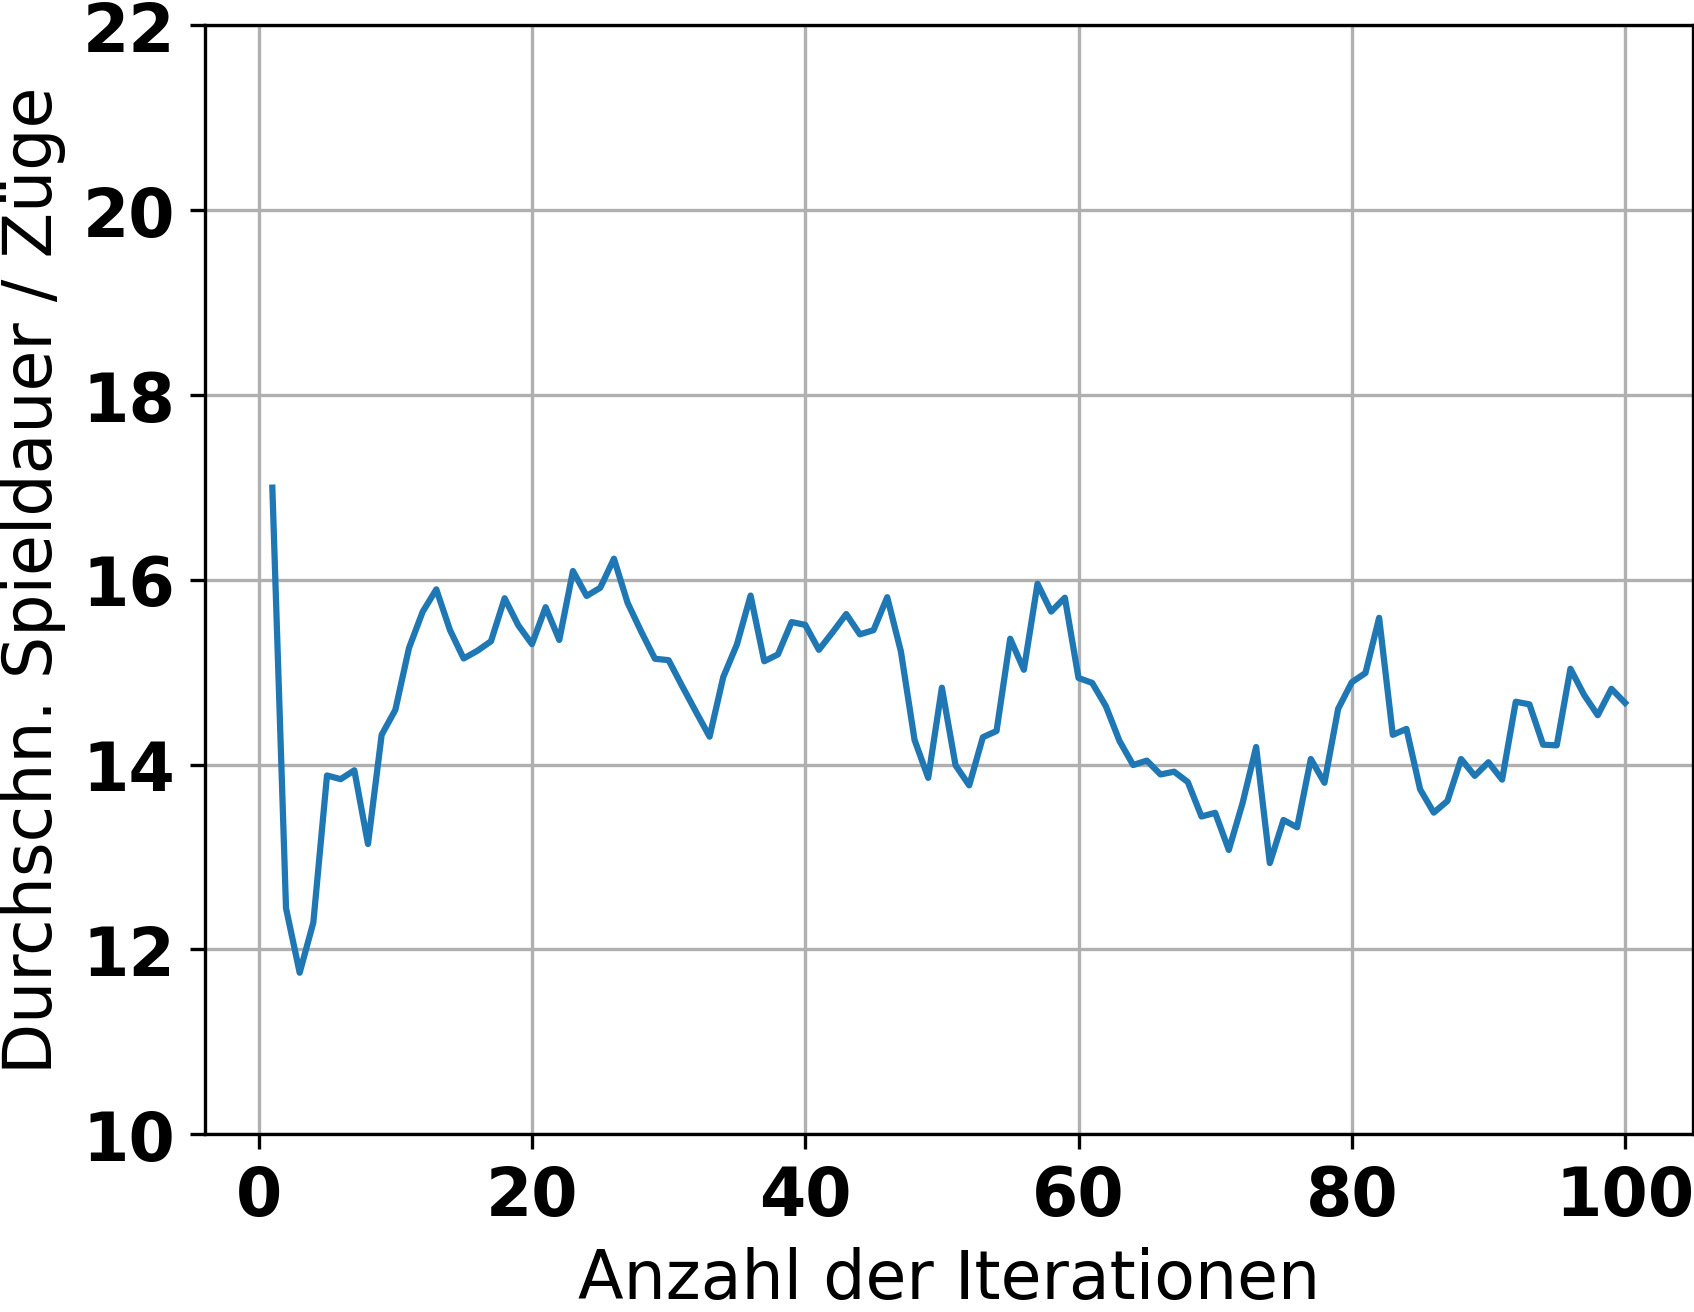
\includegraphics[width=\textwidth]{Bilder/ensemble-training/a_0_001/graph_game_lengths.png}
		\caption{Verlauf der Spieldauer mit Lernrate $\alpha_0$.}
		\label{fig:f11}
	\end{subfigure}
	\hfill
	\begin{subfigure}[b]{0.48\textwidth}
		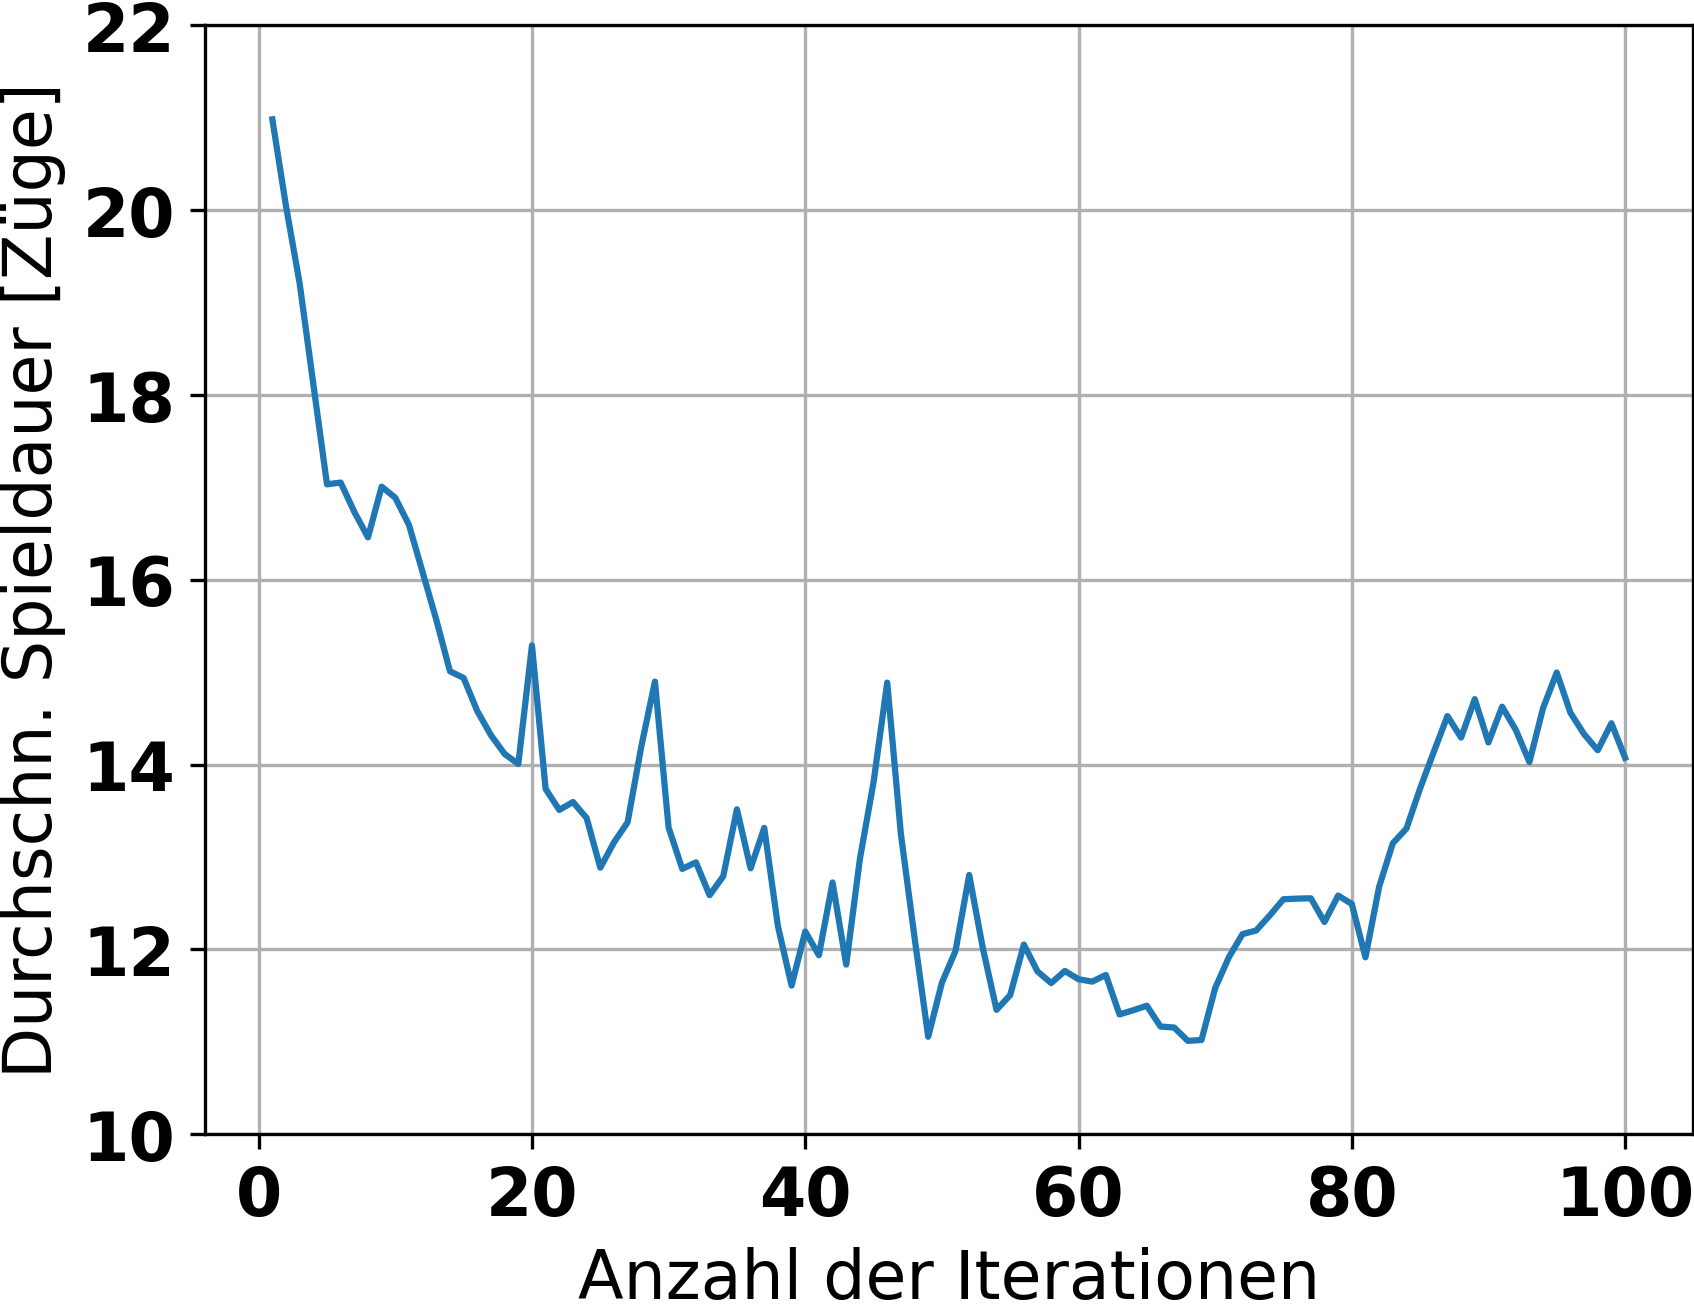
\includegraphics[width=\textwidth]{Bilder/ensemble-training/e_0_00001/graph_game_lengths.png}
		\caption{Verlauf der Spieldauer mit Lernrate $\alpha_4$.}
		\label{fig:f12}
	\end{subfigure}
	\caption{Verlauf der Spieldauer während des Trainings nach Zhong et al. mit den Lernraten $\alpha_0$ und $\alpha_4$.}
\end{figure}

Die Gewinnrate steigt bei den Trainings mit den kleineren Lernraten $\alpha_2$, $\alpha_3$ und $\alpha_4$, innerhalb der ersten 20 Iterationen und fluktuiert von dort bis zum Ende des jeweiligen Trainings auf einem konstanten Niveau. Dieses Niveau beträgt bei der Lernrate $\alpha_2$ etwa 85 \% und bei $\alpha_3$ und $\alpha_4$ etwa 80 \%. Mit den Lernraten $\alpha_0$ und $\alpha_1$ steigt die Gewinnrate nach etwa 5 Iterationen auf knapp über 90 \% und fällt danach auf etwa 80 \%.

Die durchschnittliche Spieldauer verläuft bei allen Trainings unabhängig von der Lernrate ähnlich. Die Spieldauer sinkt im Verlauf des Trainings auf knapp unter 12 Züge und steigt wieder auf zwischen 14 und 18 Züge. Der Punkt mit der niedrigsten Spieldauer tritt dabei mit kleineren Lernraten tendenziell erst nach mehr Iterationen auf.

Eine sinkende Gewinnrate bzw. eine konstante Gewinnrate mit steigender Spieldauer deuten darauf hin, dass Verhalten, das stark gegen einen zufällig spielenden Agenten ist, im Laufe des Trainings erlernt und anschließend wieder verlernt wird. Die Spielstärke des MCTS-Agenten, der gegen zufällig spielende Gegenspieler eine Gewinnrate von 100 \% und eine Spieldauer von 9 Zügen erzielt, wird im Laufe des Trainings an keiner Stelle erreicht.

Um die Ursache für das stagnierende bzw. rückläufige Lernverhalten zu ergründen, wurden der Policy-Gradient-Verlust und der Werteverlust näher betrachtet.

Bei den großen Lernraten $\alpha_0$ und $\alpha_1$, fluktuiert der Werteverlust weitgehend auf einem konstanten Niveau zwischen 0,2 und 0,4. Dieses Verhalten kann auf eine zu große Lernrate zurückzuführen sein, die dazu führt, dass die Parameter um ein Verlustminimum herum oszillieren. Bei der mittleren Lernrate $\alpha_2$ lässt sich beobachten, dass der Werteverlust vor einer konstanten Fluktuation in den ersten 20 Iterationen von 0,5 auf etwa 0,25 sinkt. Das kann ein Hinweis dafür sein, dass sich die Parameter während der ersten Iterationen auf ein lokales Minimum zu bewegen. Bei den kleineren Lernraten $\alpha_3$ und $\alpha_4$ werden kleinere Fluktuationen, dafür ein unregelmäßiges Verhalten mit Einbrüchen der Werteverluste über mehrere aufeinanderfolgende Iterationen beobachtet. Die Einbrüche erfolgen dabei teilweise für beide Spieler unterschiedlich. Plötzlich einbrechender und wieder steigender Verlust können darauf hinweisen, dass die trainierenden Modelle neues Verhalten erlernen und auf die Verhaltensänderungen voneinander reagieren.

\begin{figure}[ht!]%[!tbp]
	\begin{subfigure}[b]{0.32\textwidth}
		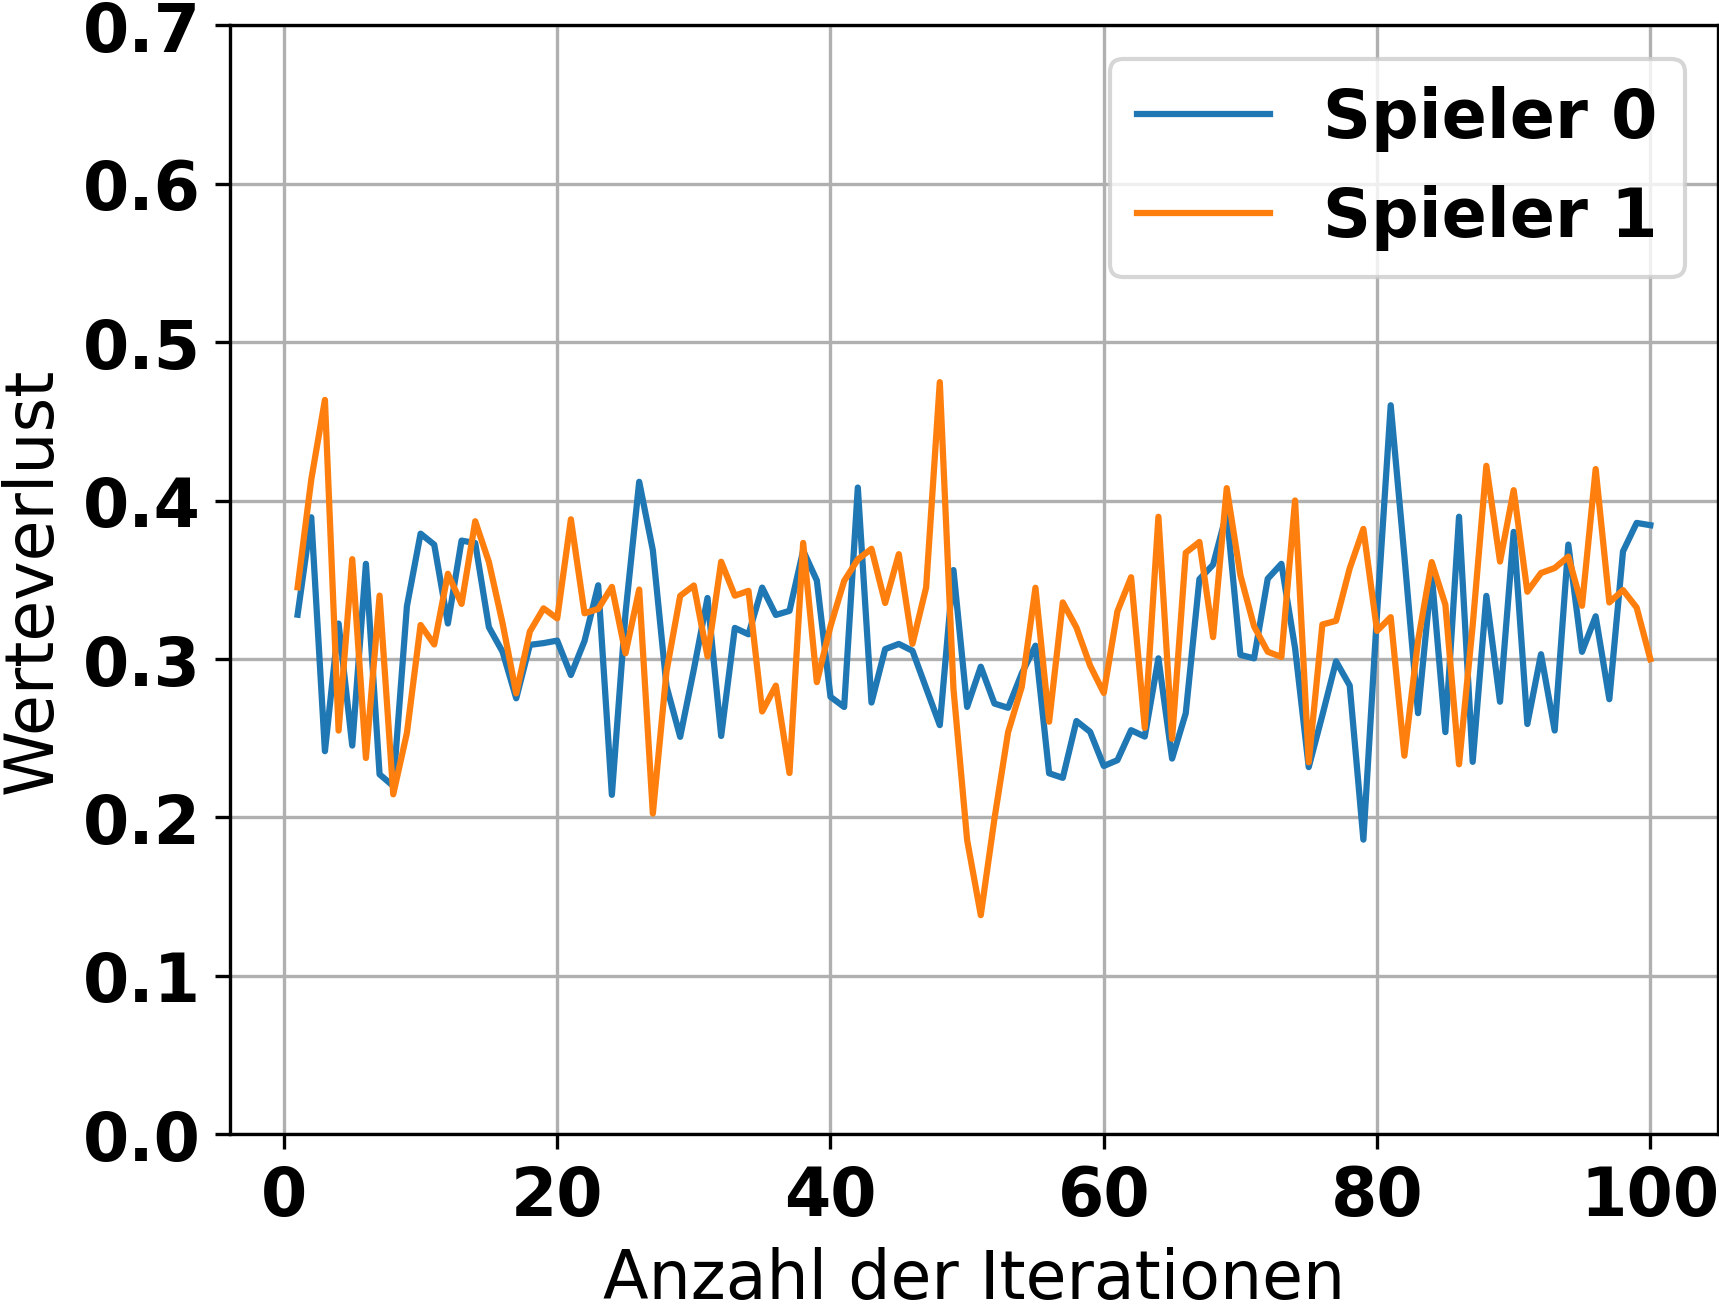
\includegraphics[width=\textwidth]{Bilder/ensemble-training/a_0_001/graph_value_losses.png}
		\caption{Verlauf des Werteverlustes mit Lernrate $\alpha_0$.}
		\label{fig:f13}
	\end{subfigure}
	\hfill
	\begin{subfigure}[b]{0.32\textwidth}
		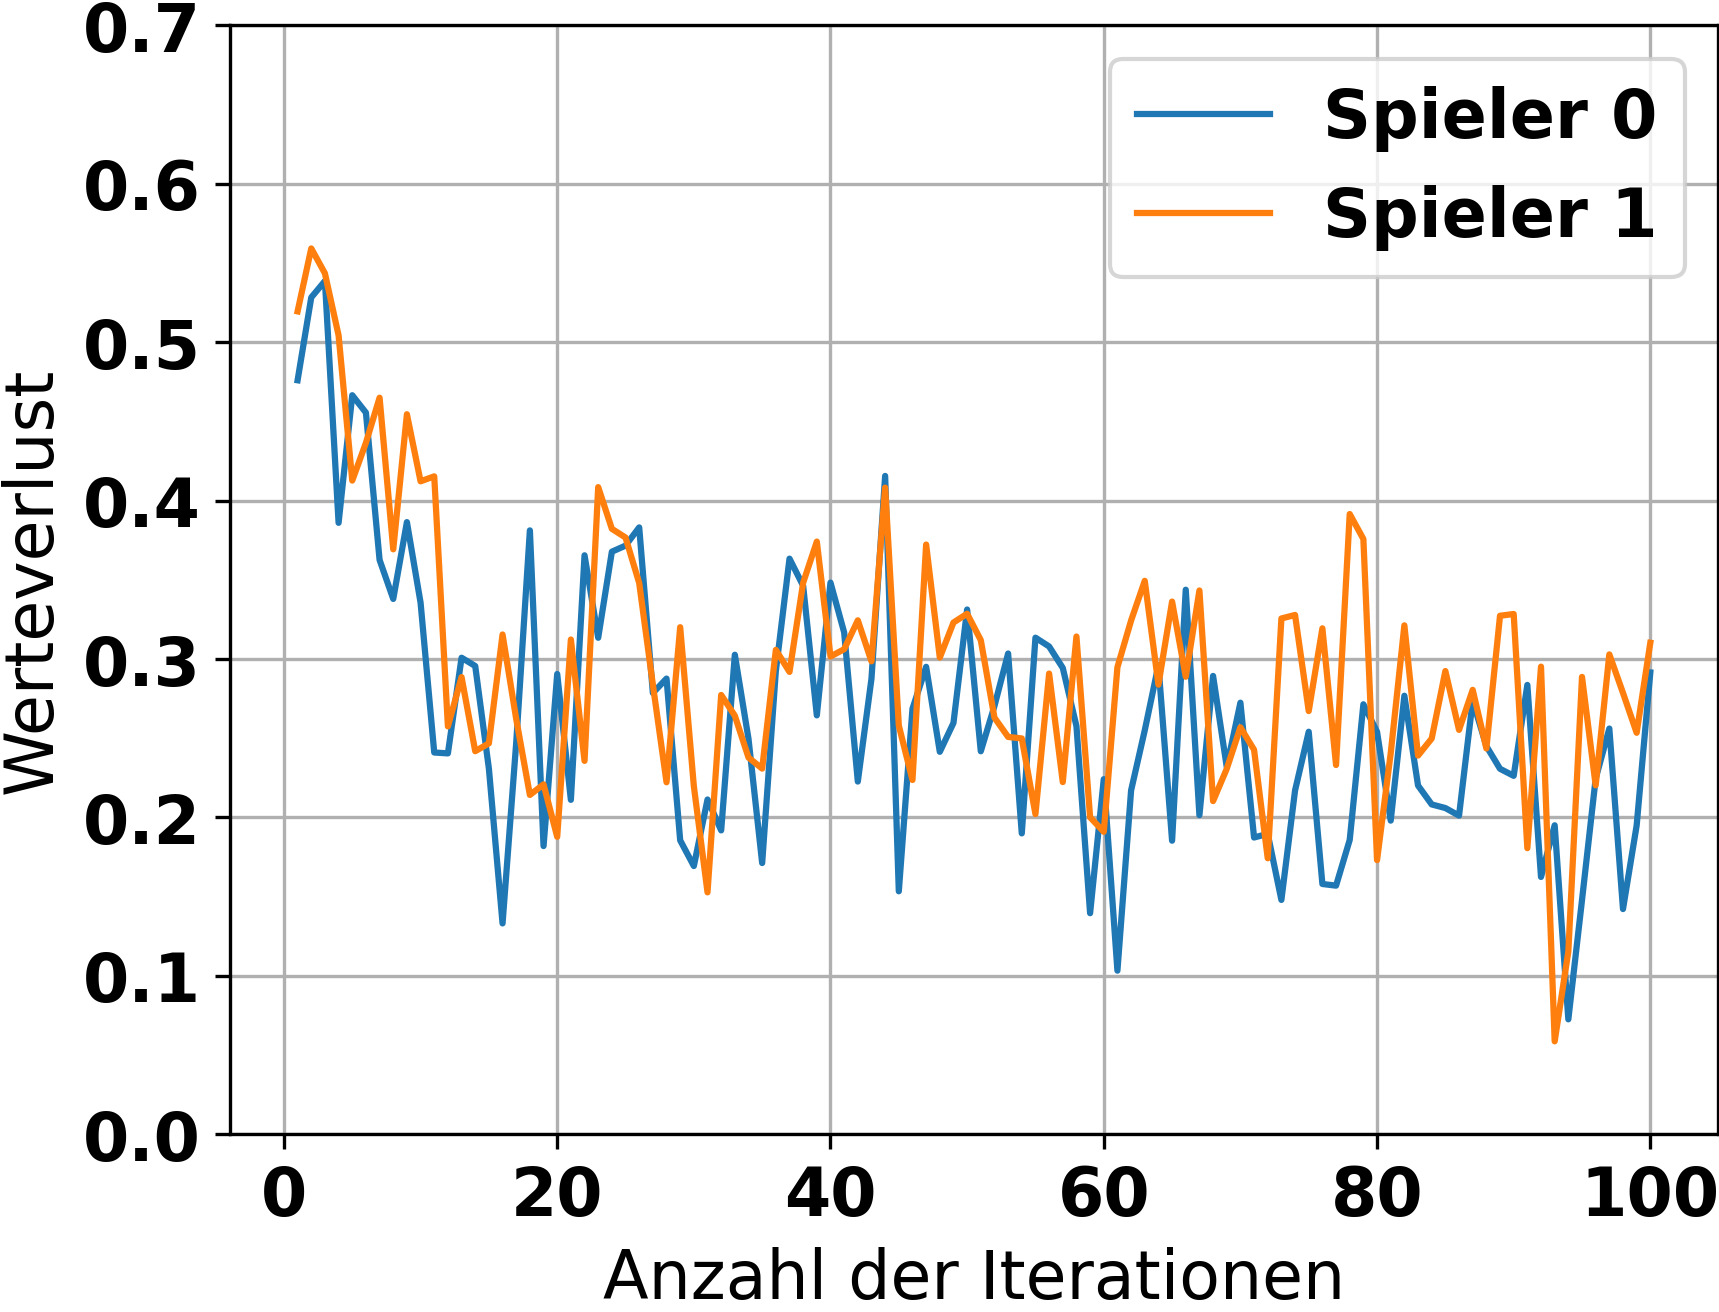
\includegraphics[width=\textwidth]{Bilder/ensemble-training/c_0_0001/graph_value_losses.png}
		\caption{Verlauf des Werteverlustes mit Lernrate $\alpha_2$.}
		\label{fig:f14}
	\end{subfigure}
	\hfill
	\begin{subfigure}[b]{0.32\textwidth}
		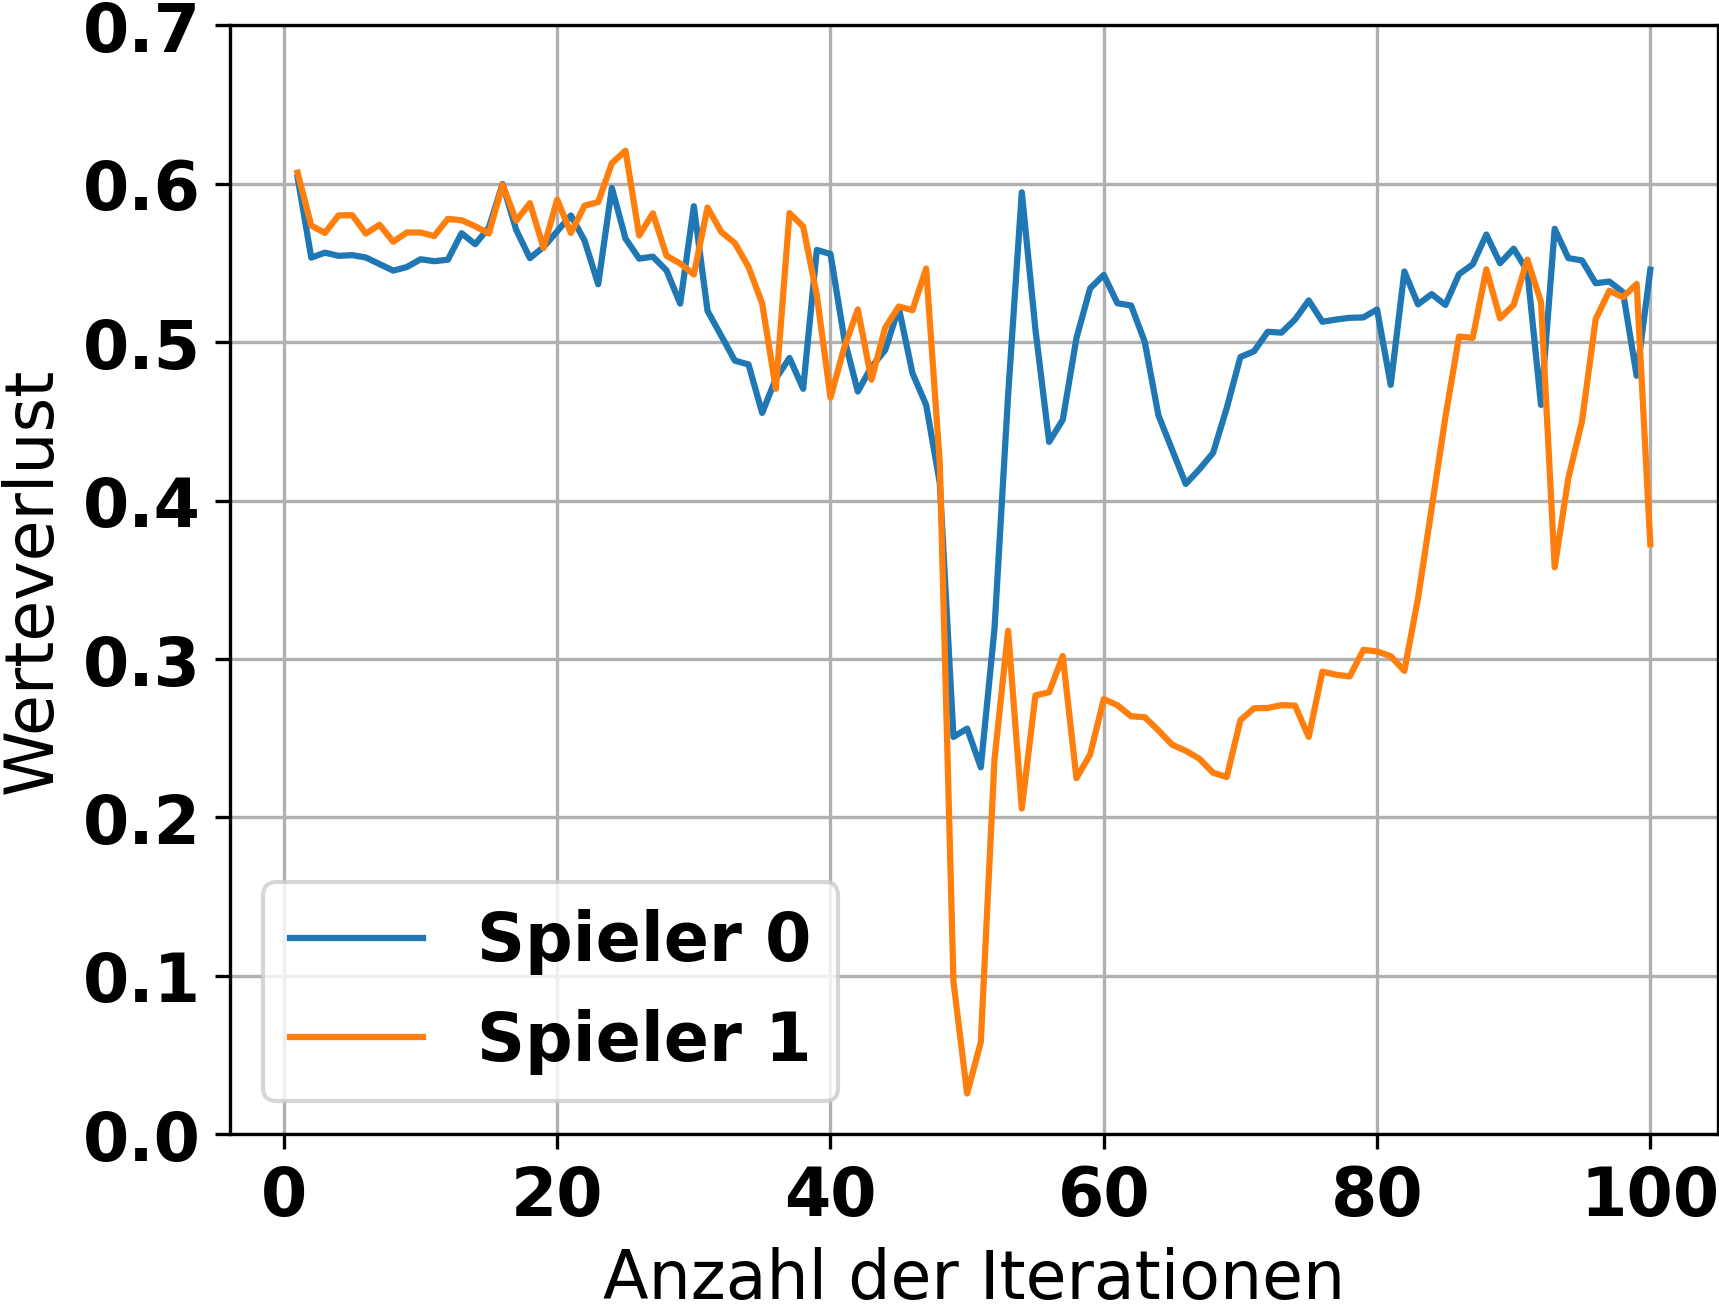
\includegraphics[width=\textwidth]{Bilder/ensemble-training/e_0_00001/graph_value_losses.png}
		\caption{Verlauf des Werteverlustes mit Lernrate $\alpha_4$.}
		\label{fig:f15}
	\end{subfigure}
	\caption{Verlauf des Werteverlustes während des Trainings nach Zhong et al. mit den Lernraten $\alpha_0$ und $\alpha_4$.}
\end{figure}

Der Policy-Gradient-Verlust fluktuiert bei den Trainings mit den Lernraten $\alpha_0$ und $\alpha_2$ über den gesamten Verlauf um einen konstanten Wert von -0,025 bzw. 0,015. Die Fluktuation um einen konstanten Wert deutet dabei auf eine zu große Lernrate hin. Bei der zweitgrößten Lernrate $\alpha_1$ wird eine Fluktuation konstanten Ausmaßes beobachtet, wobei der Wert um den fluktuiert wird, in den ersten 60 Iterationen von etwa -0,025 auf -0,010 steigt und danach auf -0,020 sinkt. Ähnlich wie beim Werteverlust bei der mittleren Lernrate $\alpha_2$ kann der sich zunächst an Null annähernde Verlust als eine positive Entwicklung interpretiert werden. Je kleiner die Lernrate ist, desto näher bewegen sich die Werte für den Policy-Gradient-Verlust bei Null und desto kleiner werden über den größten Teil des Verlaufs die Fluktuationen. Dafür treten im Verhältnis zur sinkenden Fluktuation häufiger einzelne größere Ausreißer auf. Dies kann wie der Werteverlust mit plötzlichen, länger andauernden Einbrüchen auf neu erlerntes Verhalten hindeuten.

\begin{figure}[ht!]%[!tbp]
	\begin{subfigure}[b]{0.32\textwidth}
		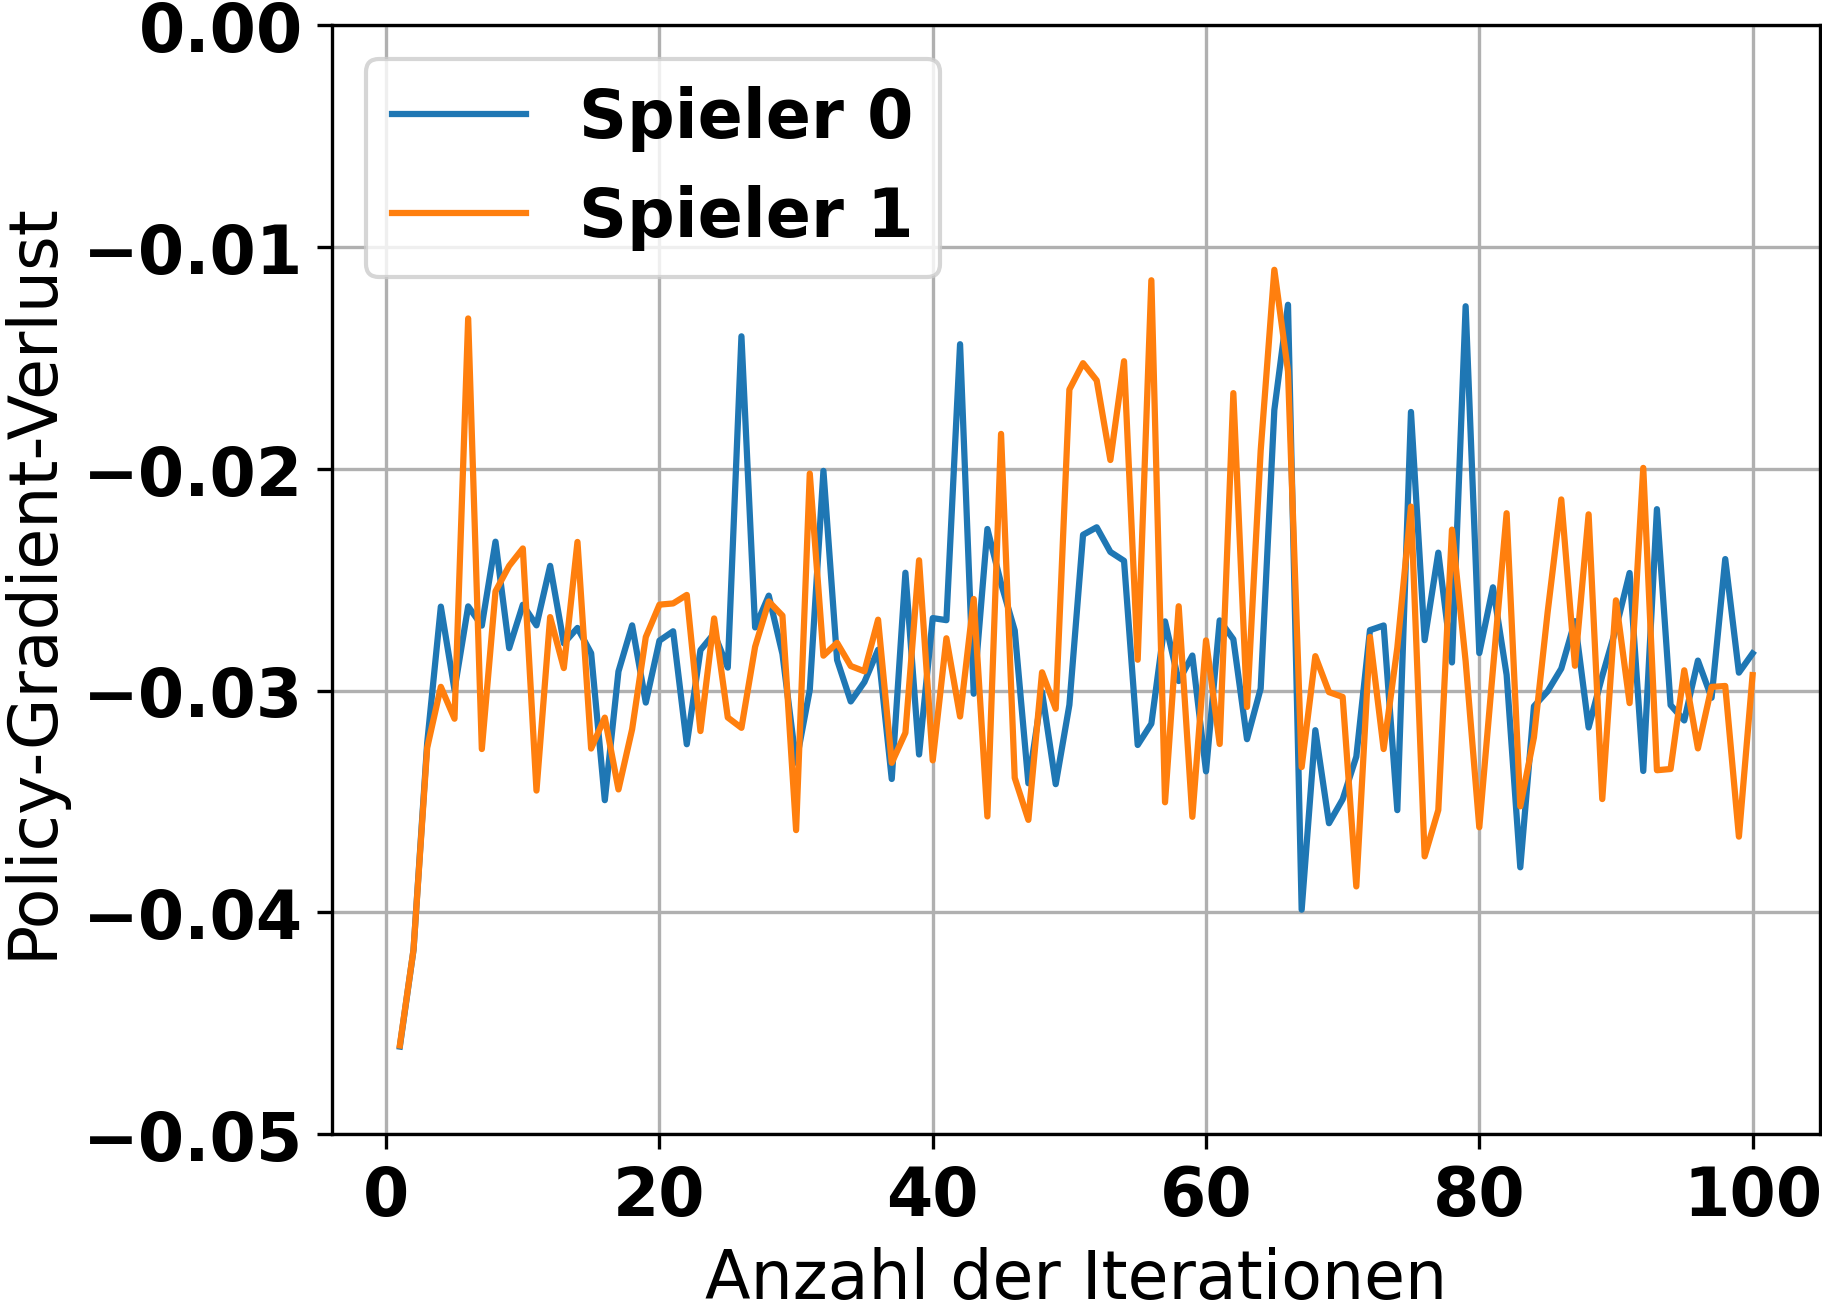
\includegraphics[width=\textwidth]{Bilder/ensemble-training/a_0_001/graph_policy_gradient_losses.png}
		\caption{Verlauf des Policy-Gradient-Verlustes mit Lernrate $\alpha_0$.}
		\label{fig:f16}
	\end{subfigure}
	\hfill
	\begin{subfigure}[b]{0.32\textwidth}
		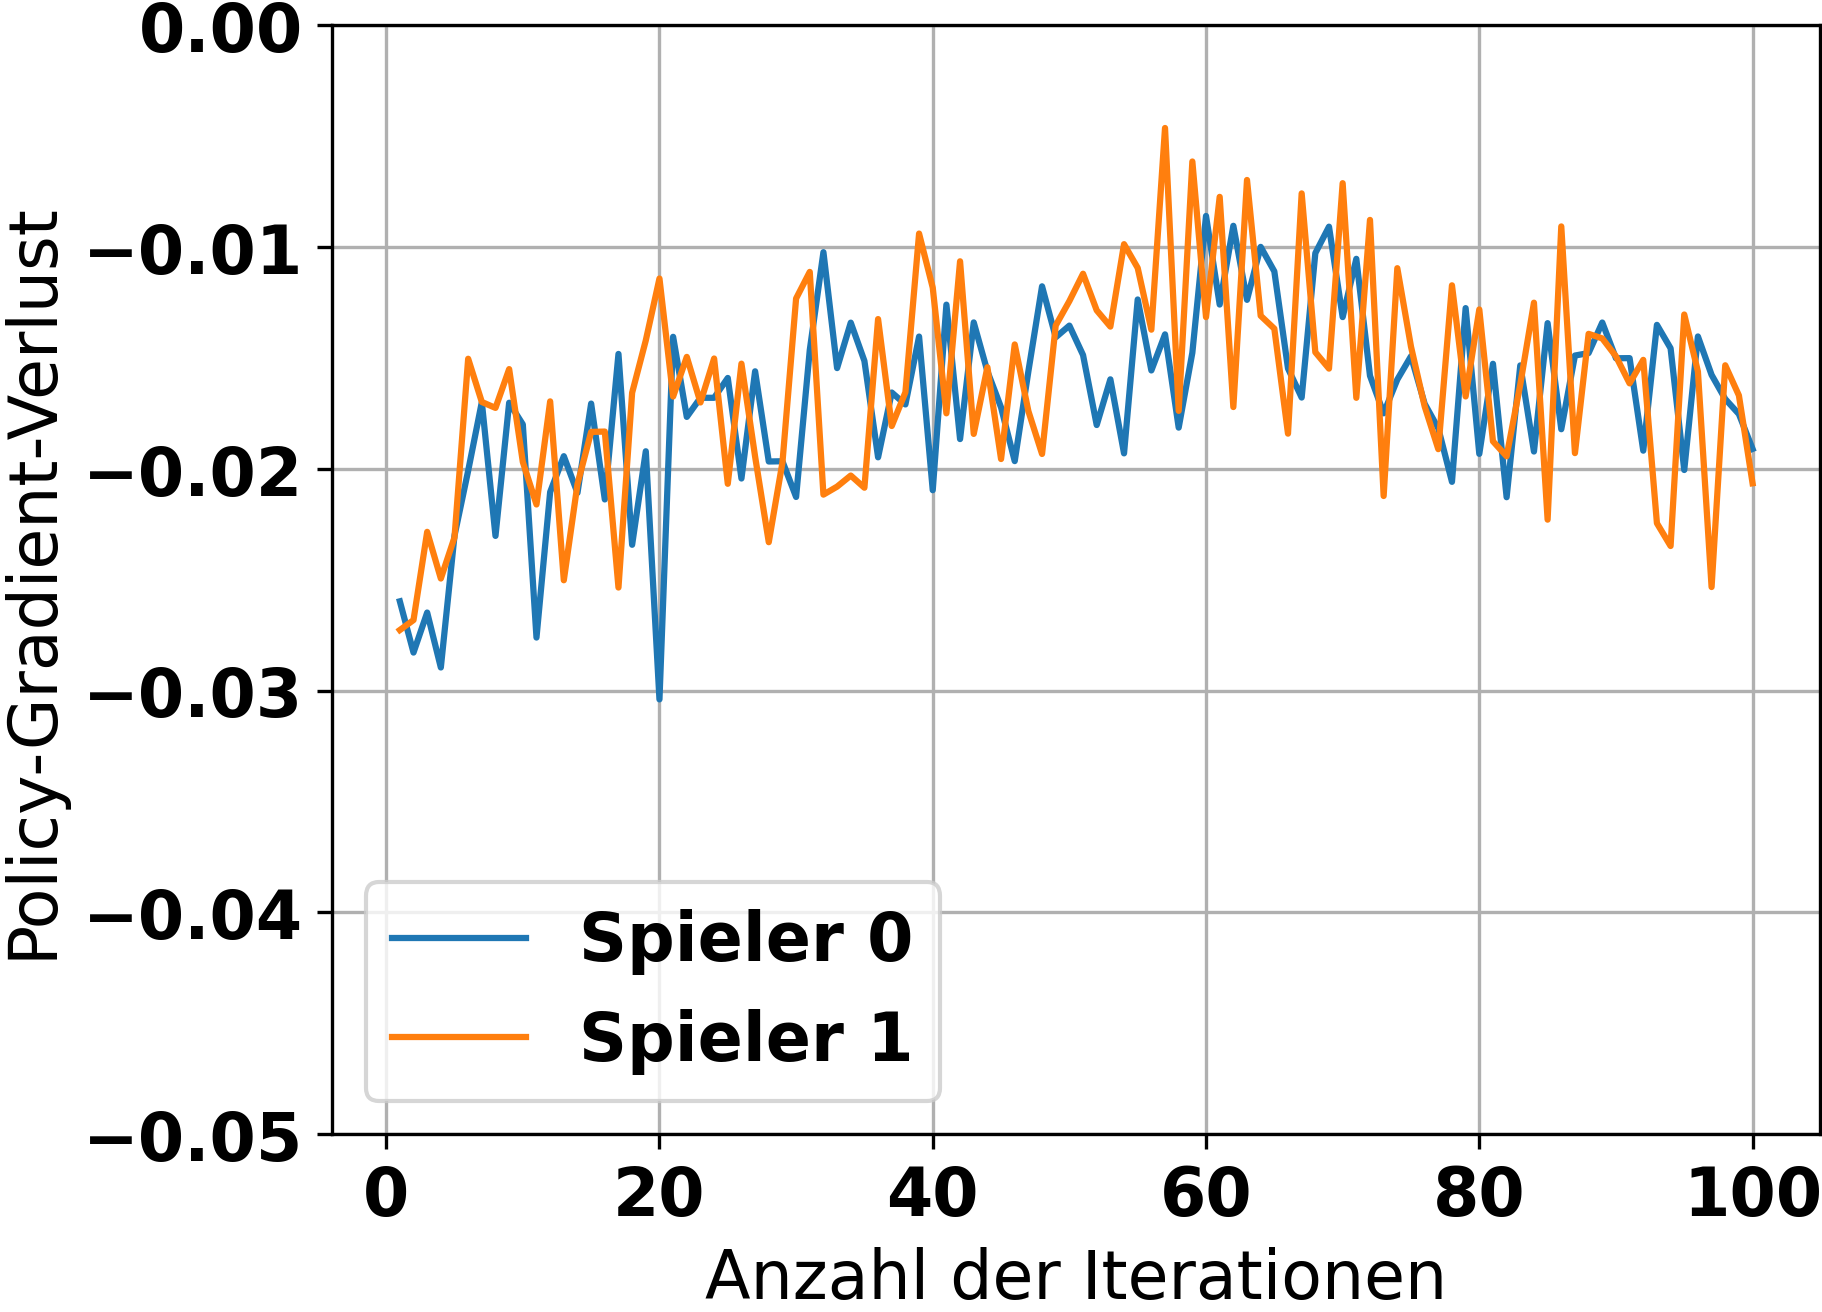
\includegraphics[width=\textwidth]{Bilder/ensemble-training/b_0_0003/graph_policy_gradient_losses.png}
		\caption{Verlauf des Policy-Gradient-Verlustes mit Lernrate $\alpha_1$.}
		\label{fig:f17}
	\end{subfigure}
	\hfill
	\begin{subfigure}[b]{0.32\textwidth}
		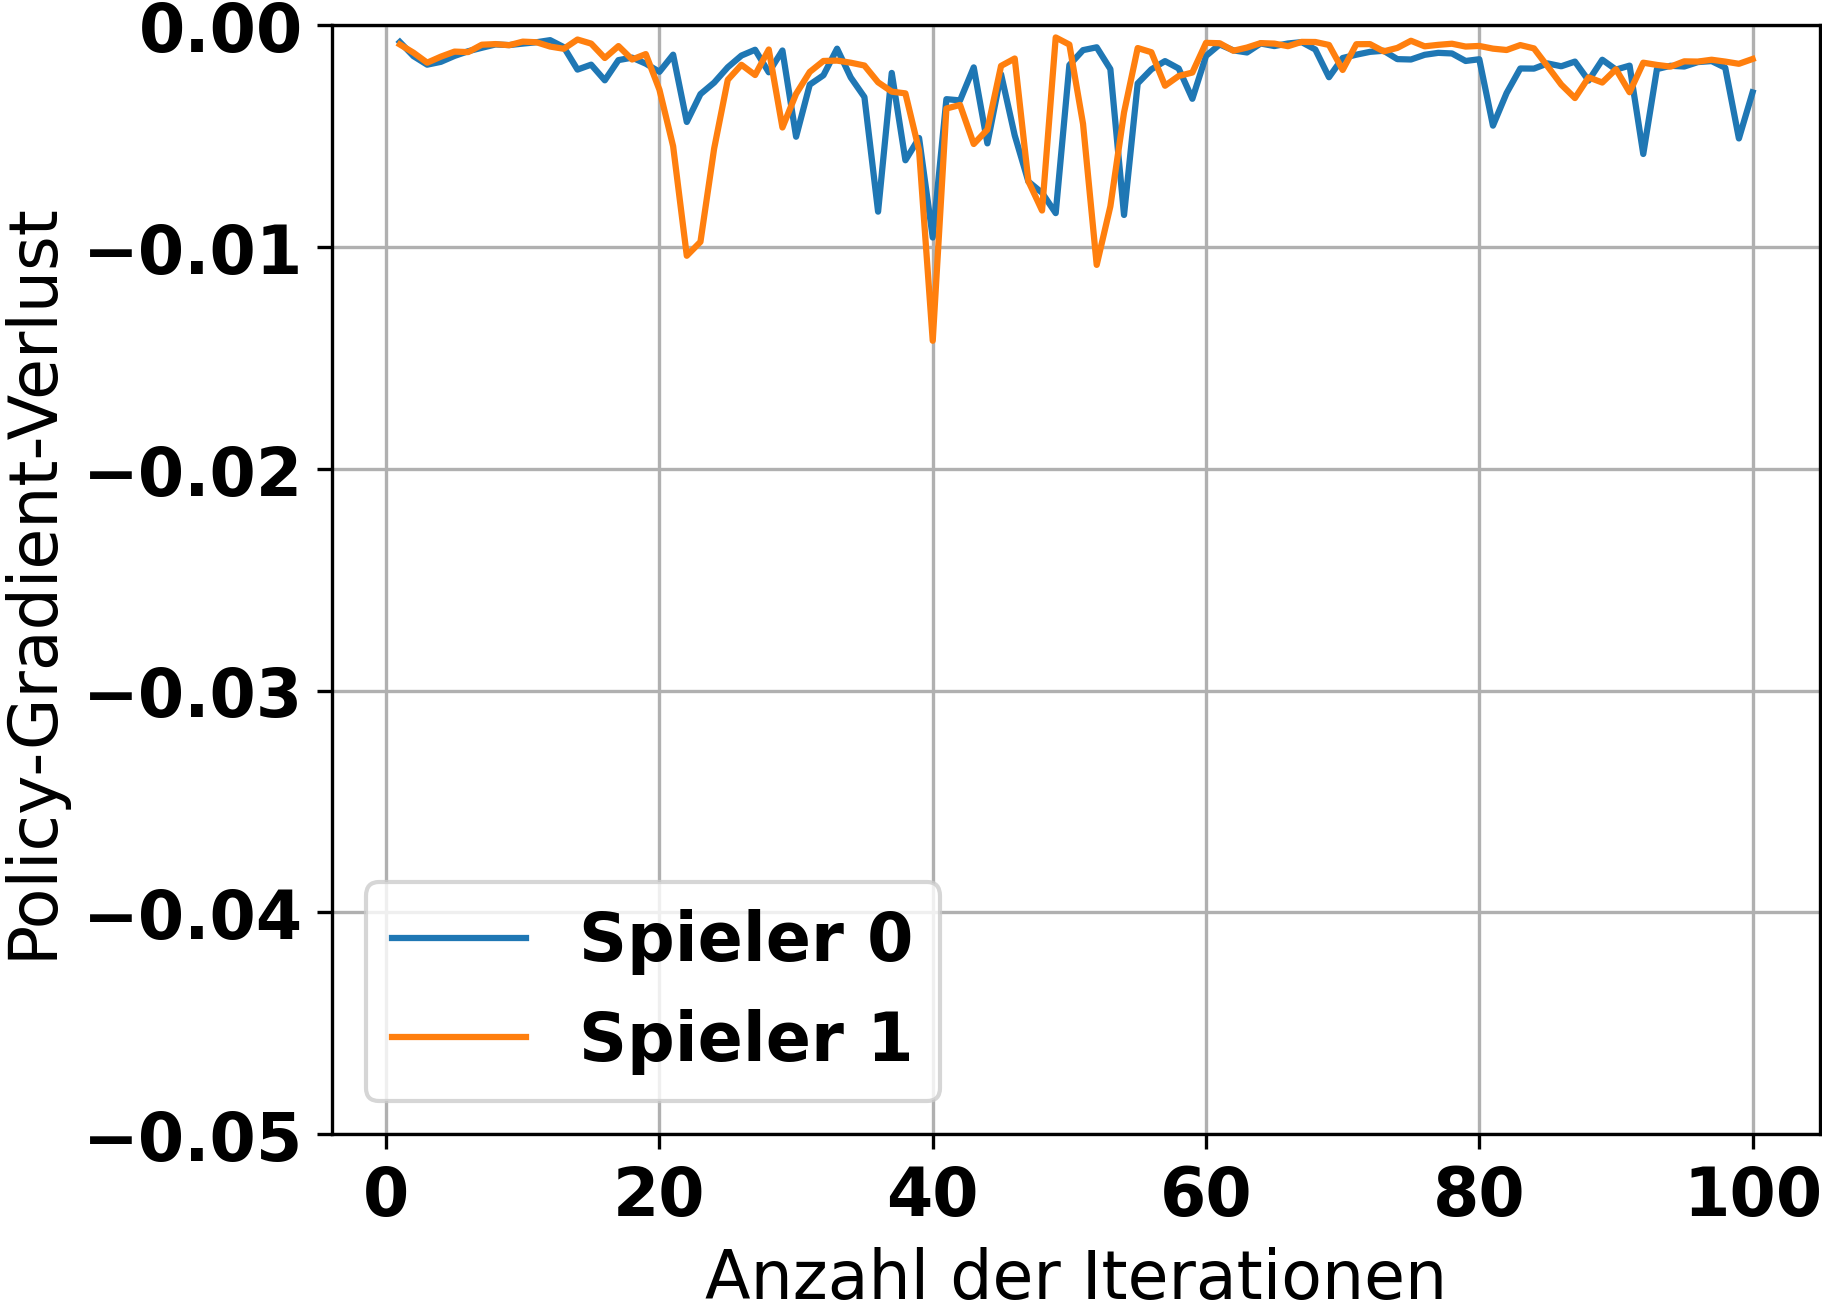
\includegraphics[width=\textwidth]{Bilder/ensemble-training/e_0_00001/graph_policy_gradient_losses.png}
		\caption{Verlauf des Policy-Gradient-Verlustes mit Lernrate $\alpha_4$.}
		\label{fig:f18}
	\end{subfigure}
	\caption{Verlauf des Policy-Gradient-Verlustes während des Trainings nach Zhong et al. mit den Lernraten $\alpha_0$, $\alpha_1$ und $\alpha_4$.}
\end{figure}

Leider wurden keine Korrelationen zwischen dem Verhalten des Policy-Gradient- oder Werteverlustes und der Leistung der trainierten Modell hinsichtlich Gewinnrate oder Spieldauer gefunden. Es lassen sich daher auch keine Aussagen darüber treffen, ob fluktuierende Verlust-Verläufe, die sich über die Iterationen der 0 annähern oder weniger fluktuierende Verläufe mit plötzlichen Einbrüchen oder Ausreißern erstrebenswerter sind. Um die Ursachen für das stagnierende Training weiter zu ergründen, sind die Analyse von weiteren Trainingsmetriken und Experimente mit weiteren Hyperparametern erforderlich.

Anstatt nur den Verlauf der mittleren Verluste der einzelnen Iterationen, und die Leistung gegen den zufälligen Agenten am Ende der Iterationen zu beobachten, könnte es helfen, mehr über den Verlauf der Verluste und Belohnung innerhalb der Iterationen zu erfahren. Dies wäre möglich, indem die Verluste und die mittlere in den Episoden erhaltene Belohnung über die einzelnen Trainingsschritte aufgezeichnet werden. Eine weitere hilfreiche Trainingsmetrik könnte die Entropie der Wahrscheinlichkeitsverteilungen über die Aktionen sein, die durch das Regelwerk generiert werden. Eine hohe Entropie bedeutet, dass alle Aktionen mit ähnlich großer Wahrscheinlichkeit gewählt werden, während eine niedrige Entropie bedeutet, dass wenige verschiedene Aktionen mit hoher Wahrscheinlichkeit gewählt werden. Sie ist ein Maß dafür, wie sicher sich das Regelwerk in seinen Entscheidungen ist und sollte über den Verlauf des Trainings sinken \cite{Lapan.2020}.

Um das RL-Modell für Gomoku zu trainieren, wurden in \cite{Zhong.2020} neuronale Netzwerke mit Faltungsmatritzen in den ersten Netzwerkschichten eingesetzt, die bei der Erkennung von Mustern in Eingabedaten unterstützen. Trotz der niedrigeren Komplexität ist dies bei Vier Gewinnt möglicherweise ebenfalls notwendig, um starke Agenten zu trainieren. In \cite{Wäldchen.2022} wurde mit einem mit Faltungsmatritzen ausgestattetes PPO-Modell erfolgreich trainiert, sodass es gegen einen MCTS-Agenten standhalten konnte, der 2000 Simulationen pro Zug durchführt. In \cite{Thill.2012} wurden N-Tupel-Netzwerke eingesetzt, welche ebenfalls Mechanismen zur Mustererkennung enthalten. Dabei konnte ein RL-Modell trainiert werden, das als erster Spieler mit einer Wahrscheinlichkeit von 90 \% gegen einen perfekt spielenden Minimax-Agenten gewinnt.

In \cite{Taylor.2024} wurden keine Mechanismen zur Mustererkennung eingesetzt und der darin trainierte Q-Learning-Agent erzielt in Vier Gewinnt eine Gewinnrate von lediglich 80 \%. Das muss jedoch nicht an der fehlenden Mustererkennung liegen. Wie der Author selbst erwähnt, liegt das vermutlich an der fehlenden Fähigkeit des Q-Learning-Verfahrens zu verallgemeinern. Aus der Literatur geht nicht hervor, dass Faltungsmatritzen erforderlich sind, um ein starkes PPO-Modell für Vier Gewinnt zu trainieren, aber es liegt nahe, dass deren Einsatz gewinnbringend sein könnte.

\paragraph{Training gegen einen zufällig spielenden Agenten}

\label{training-random}

Aufgrund begrenzter zeitlicher Ressourcen war es nicht möglich, weitere Trainingsmetriken zu analysieren oder zusätzliche Experimente mit anderen Hyperparametern wie Netzwerkarchitekturen mit Faltungsmatritzen durchzuführen. Daher wurde die Entscheidung getroffen, auf eine einfachere Trainingsstrategie umzustellen. Sie besteht darin, ein RL-Modell gegen einen zufällig spielenden Agenten zu trainieren. Auch hier wird als RL-Verfahren PPO eingesetzt. Es wurden verschiedene Trainings mit den Lernraten $\alpha_0 = 0.003$, $\alpha_1 = 0.001$, $\alpha_2 = 0.0005$ und $\alpha_3 = 0.0001$ durchgeführt. Jedes Training war 1.024.000 Trainingsschritte lang. Alle anderen Parameter, wie die Architektur der Netzwerke oder die Anzahl der Schritte, nach denen die Gewichte des Modells angepasst werden, wurden bei den durch Stable Baselines3 voreingestellten Parameter belassen.

Beobachtet wurden dabei die durchschnittlich in den vergangenen 100 Episoden erhaltene Belohnung und die durchschnittliche Länge der Episoden. Eine Episode bezeichnet in diesem Fall ein Spiel, das im Training vom Anfang bis zum Ende durchgespielt wurde. Das trainierende Modell erhält von der PettingZoo-Umgebung eine Belohnung von 1 für Züge, die zum Gewinn geführt haben, -1 für Züge, die zum Verlust geführt haben und 0 für alle anderen Züge \cite{Farama.2025}. Die Episodenlänge bezeichnet die Anzahl der im Training durchgeführten Schritte, bis eine Episode endet. Wie in \ref{wrapper} erwähnt, besteht ein Schritt aus einer Aktion des trainierenden Modells und einer Aktion seines Gegenspielers, dem zufällig spielendem Agenten. Da die Spieler im Training nach jedem Spiel das Anzugsrecht wechseln, beträgt hier das Minimum 3,5, da mindestens 7 Steine platziert sein müssen, damit ein Spieler seine Spielteine in einer Viererkette platziert haben kann und das Spiel endet. Das Maximum ist die Hälfte Anzahl der Spielfelder, also 21. Kürzere Episoden deuten darauf hin, dass der trainierende Agent im Training stärker ist.

\begin{figure}[ht!]
	\begin{subfigure}[b]{0.48\textwidth}
		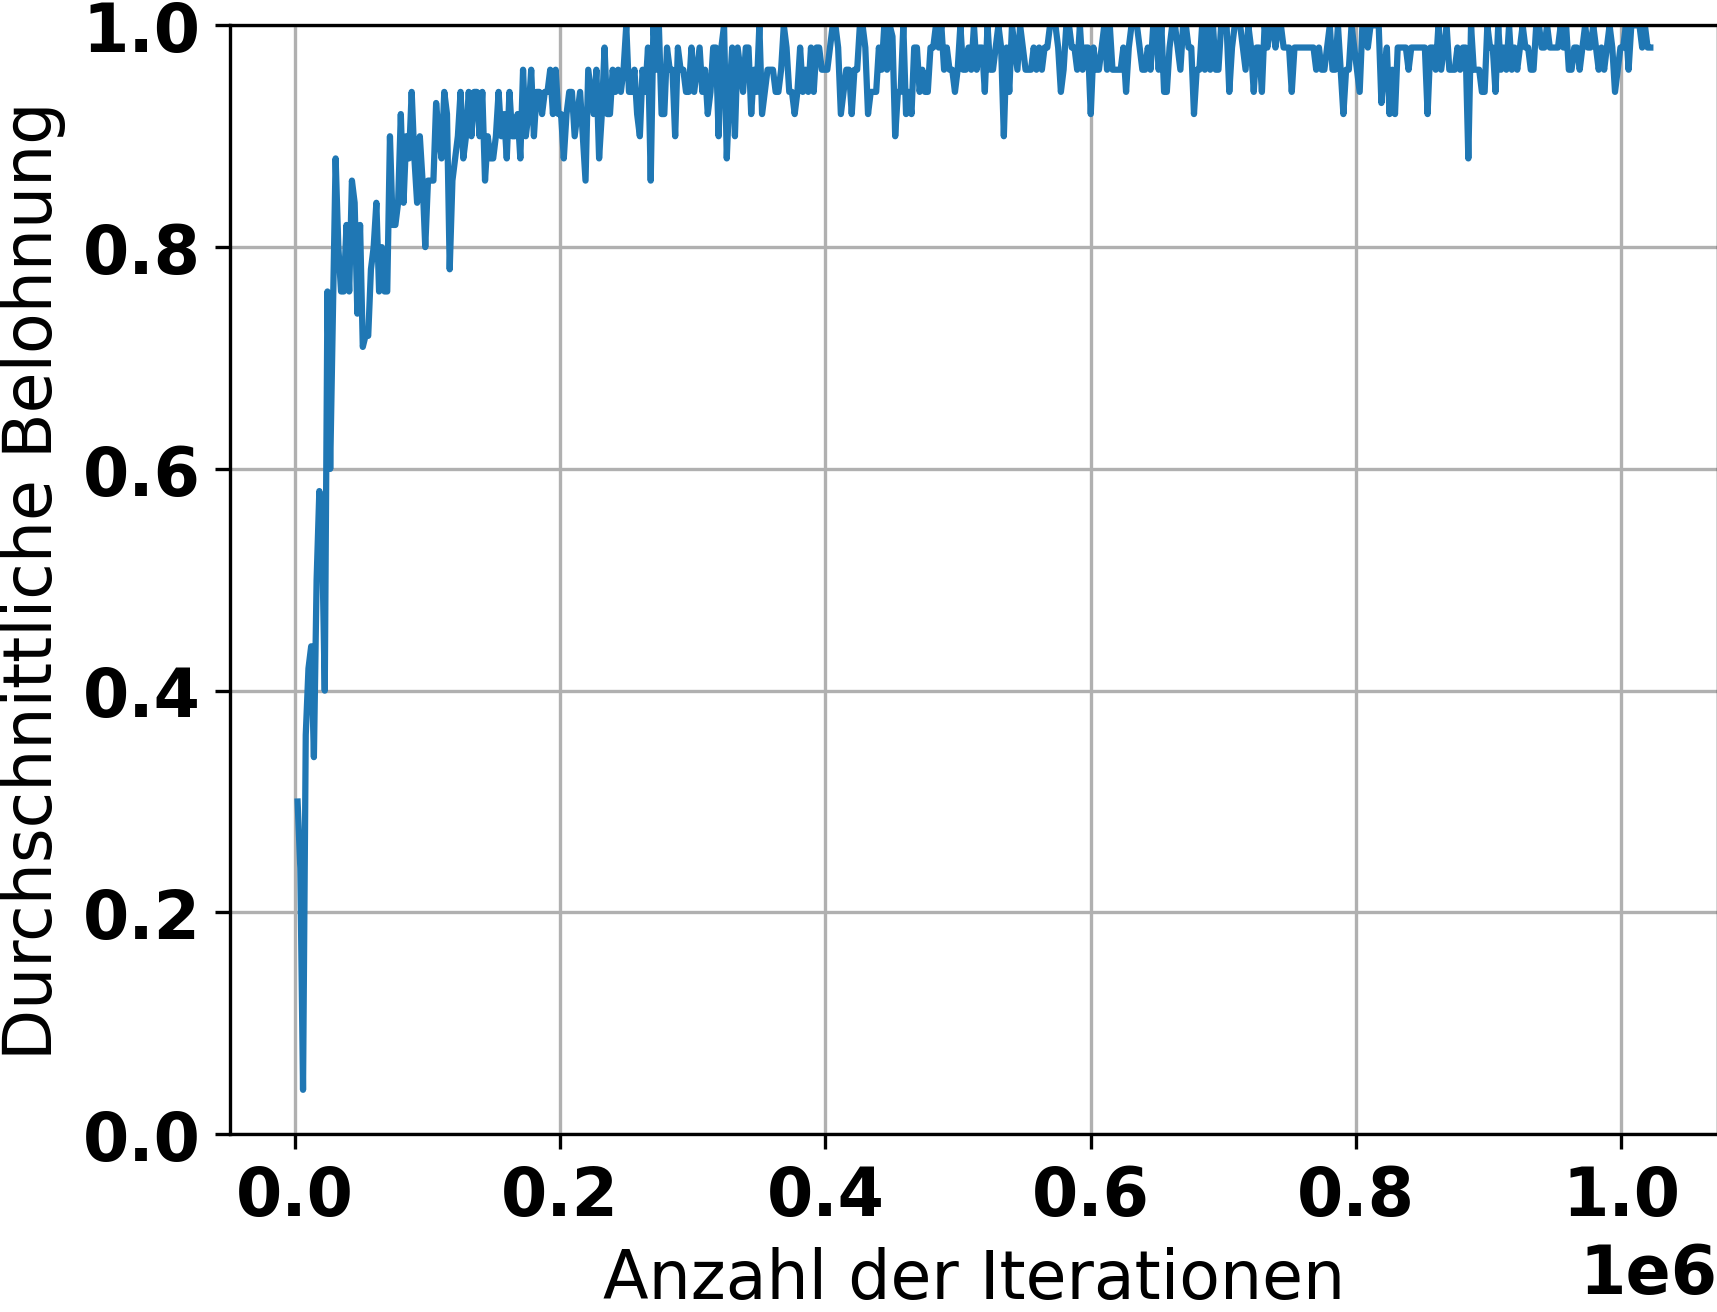
\includegraphics[width=\textwidth]{Bilder/random-training/history_random_0_0001_graph_episode_rewards.png}
		\caption{Durchschnittliche Belohnung.}
		\label{fig:f19}
	\end{subfigure}
	\hfill
	\begin{subfigure}[b]{0.48\textwidth}
		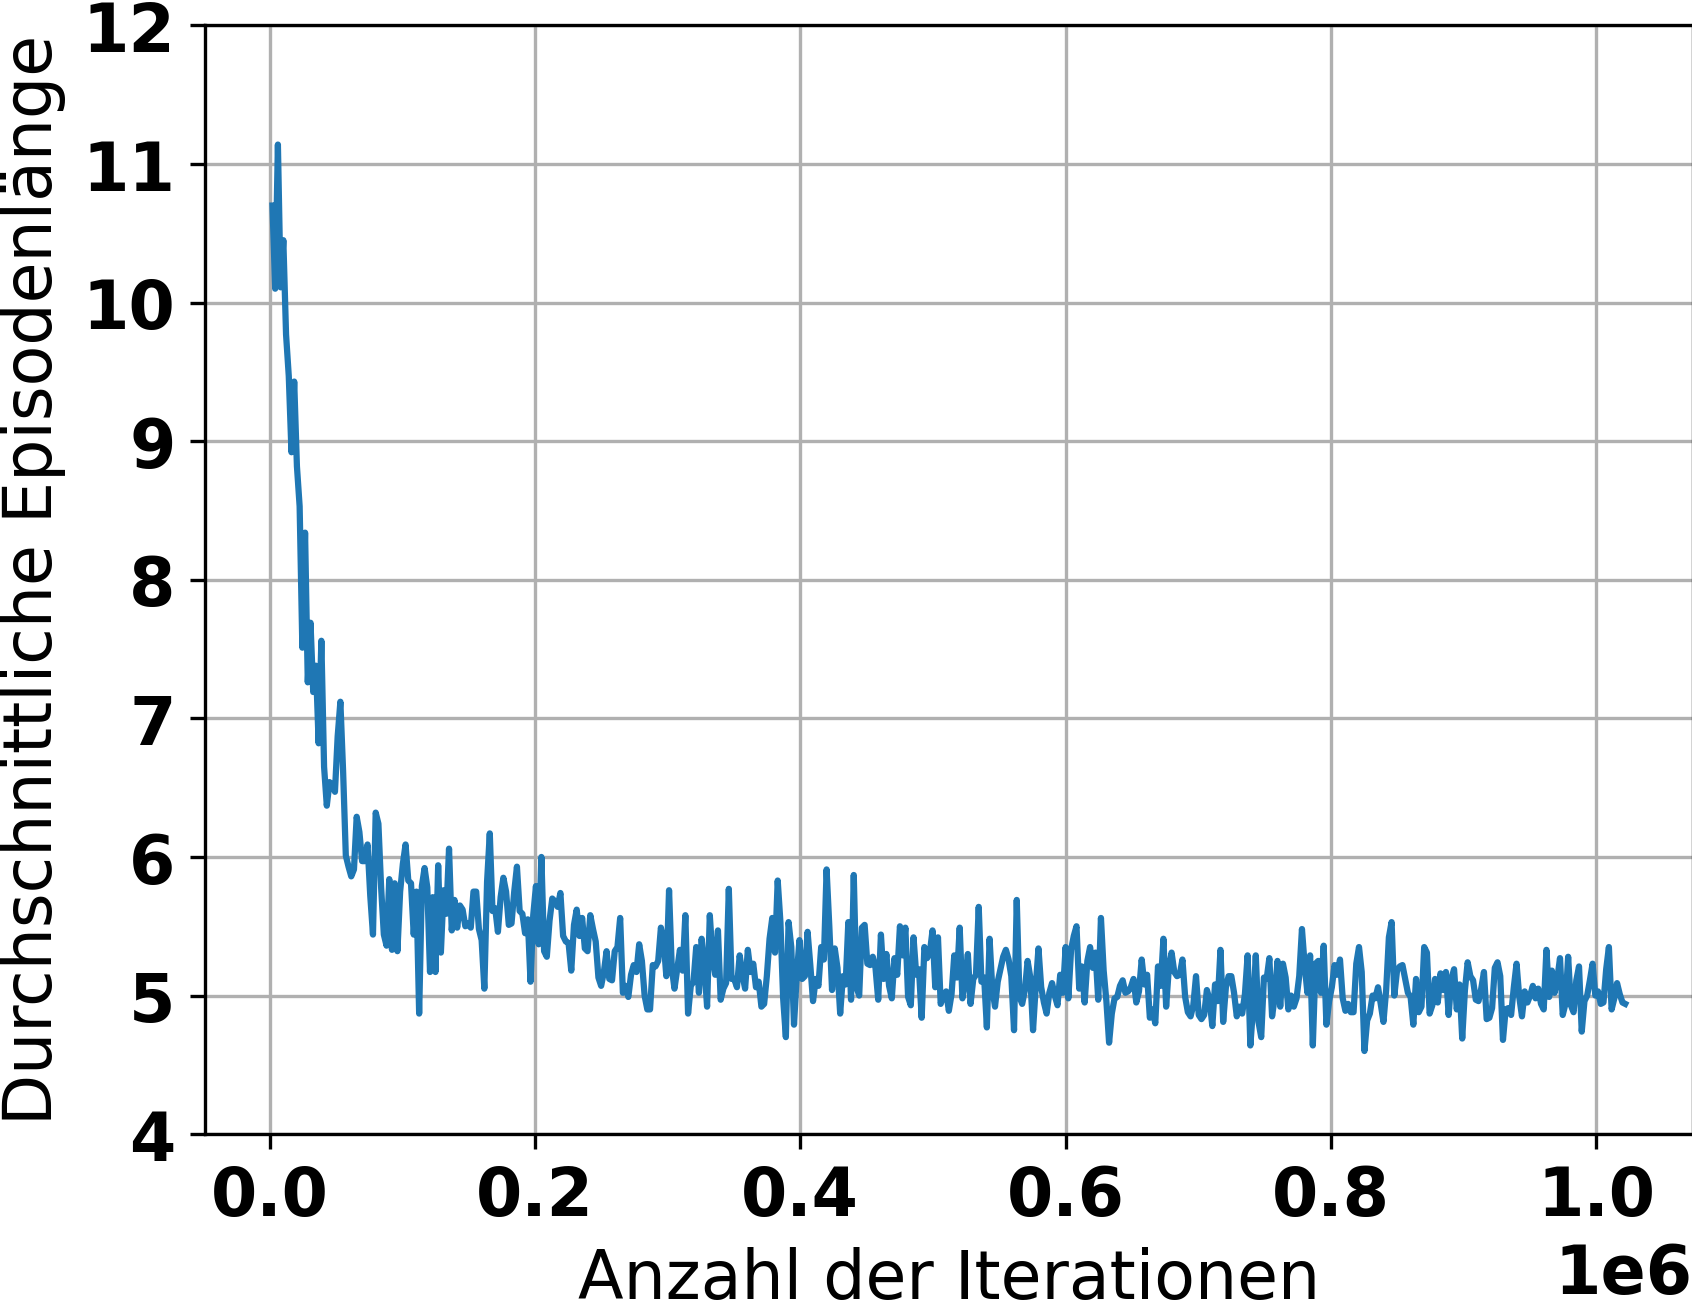
\includegraphics[width=\textwidth]{Bilder/random-training/history_random_0_0001_graph_episode_lengths.png}
		\caption{Durchschnittliche Episodenlänge.}
		\label{fig:f20}
	\end{subfigure}
	\caption{Verlauf der durchschnittlichen Belohnung und Episodenlänge während des Trainings gegen einen zufällig spielenden Agenten mit Lernrate $\alpha_3$.}
\end{figure}

Unabhängig von der Lernrate ist bei den betrachteten Trainingsmetriken nach wenigen hunderttausend Trainingsschritten ein erstrebenswertes Konvergenzverhalten zu beobachten. Die durchschnittliche in den Episoden erhaltene Belohnung konvergiert zu 1, was bedeutet, dass das Modell im Training die meisten Spiele gewinnt. Die durchschnittliche Episodenlänge konvergiert bei etwa 4,5 bis 5, was 9 bis 10 Zügen entspricht. Ergänzend zu Abbildungen \ref{fig:f19} und \ref{fig:f20} befinden sich Diagramme zu den Trainings mit den Lernraten $\alpha_0$ bis $\alpha_2$ im Anhang \ref{appendix-training-random}.

\begin{figure}[ht!]%[!tbp]
	\begin{subfigure}[b]{0.48\textwidth}
		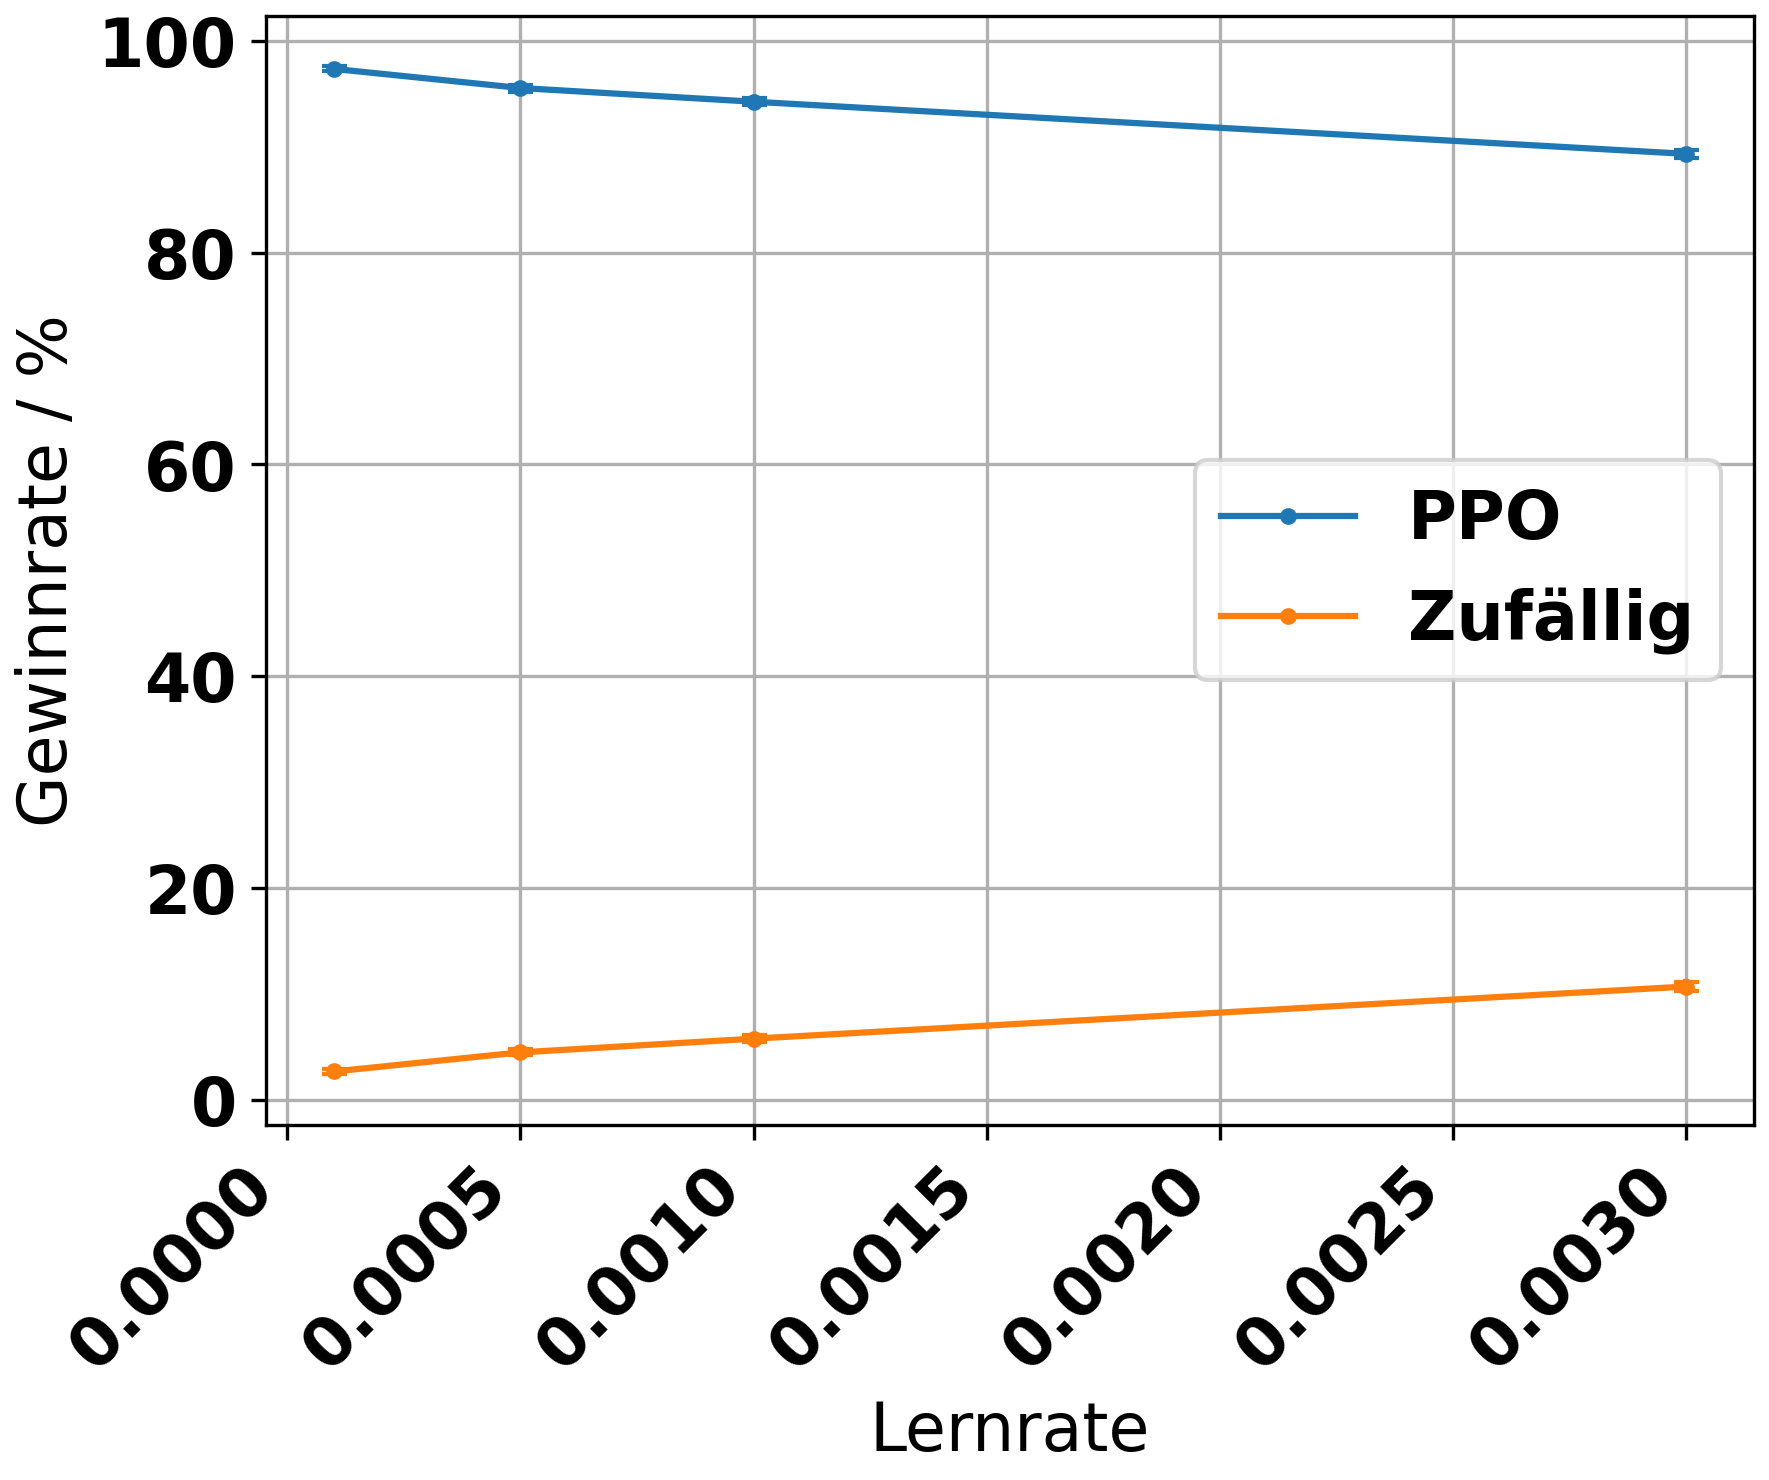
\includegraphics[width=\textwidth]{Bilder/ppo_vs_random_win_rate_vs_learning_rate.png}
		\caption{Gewinnrate.}
		\label{fig:f21}
	\end{subfigure}
	\hfill
	\begin{subfigure}[b]{0.48\textwidth}
		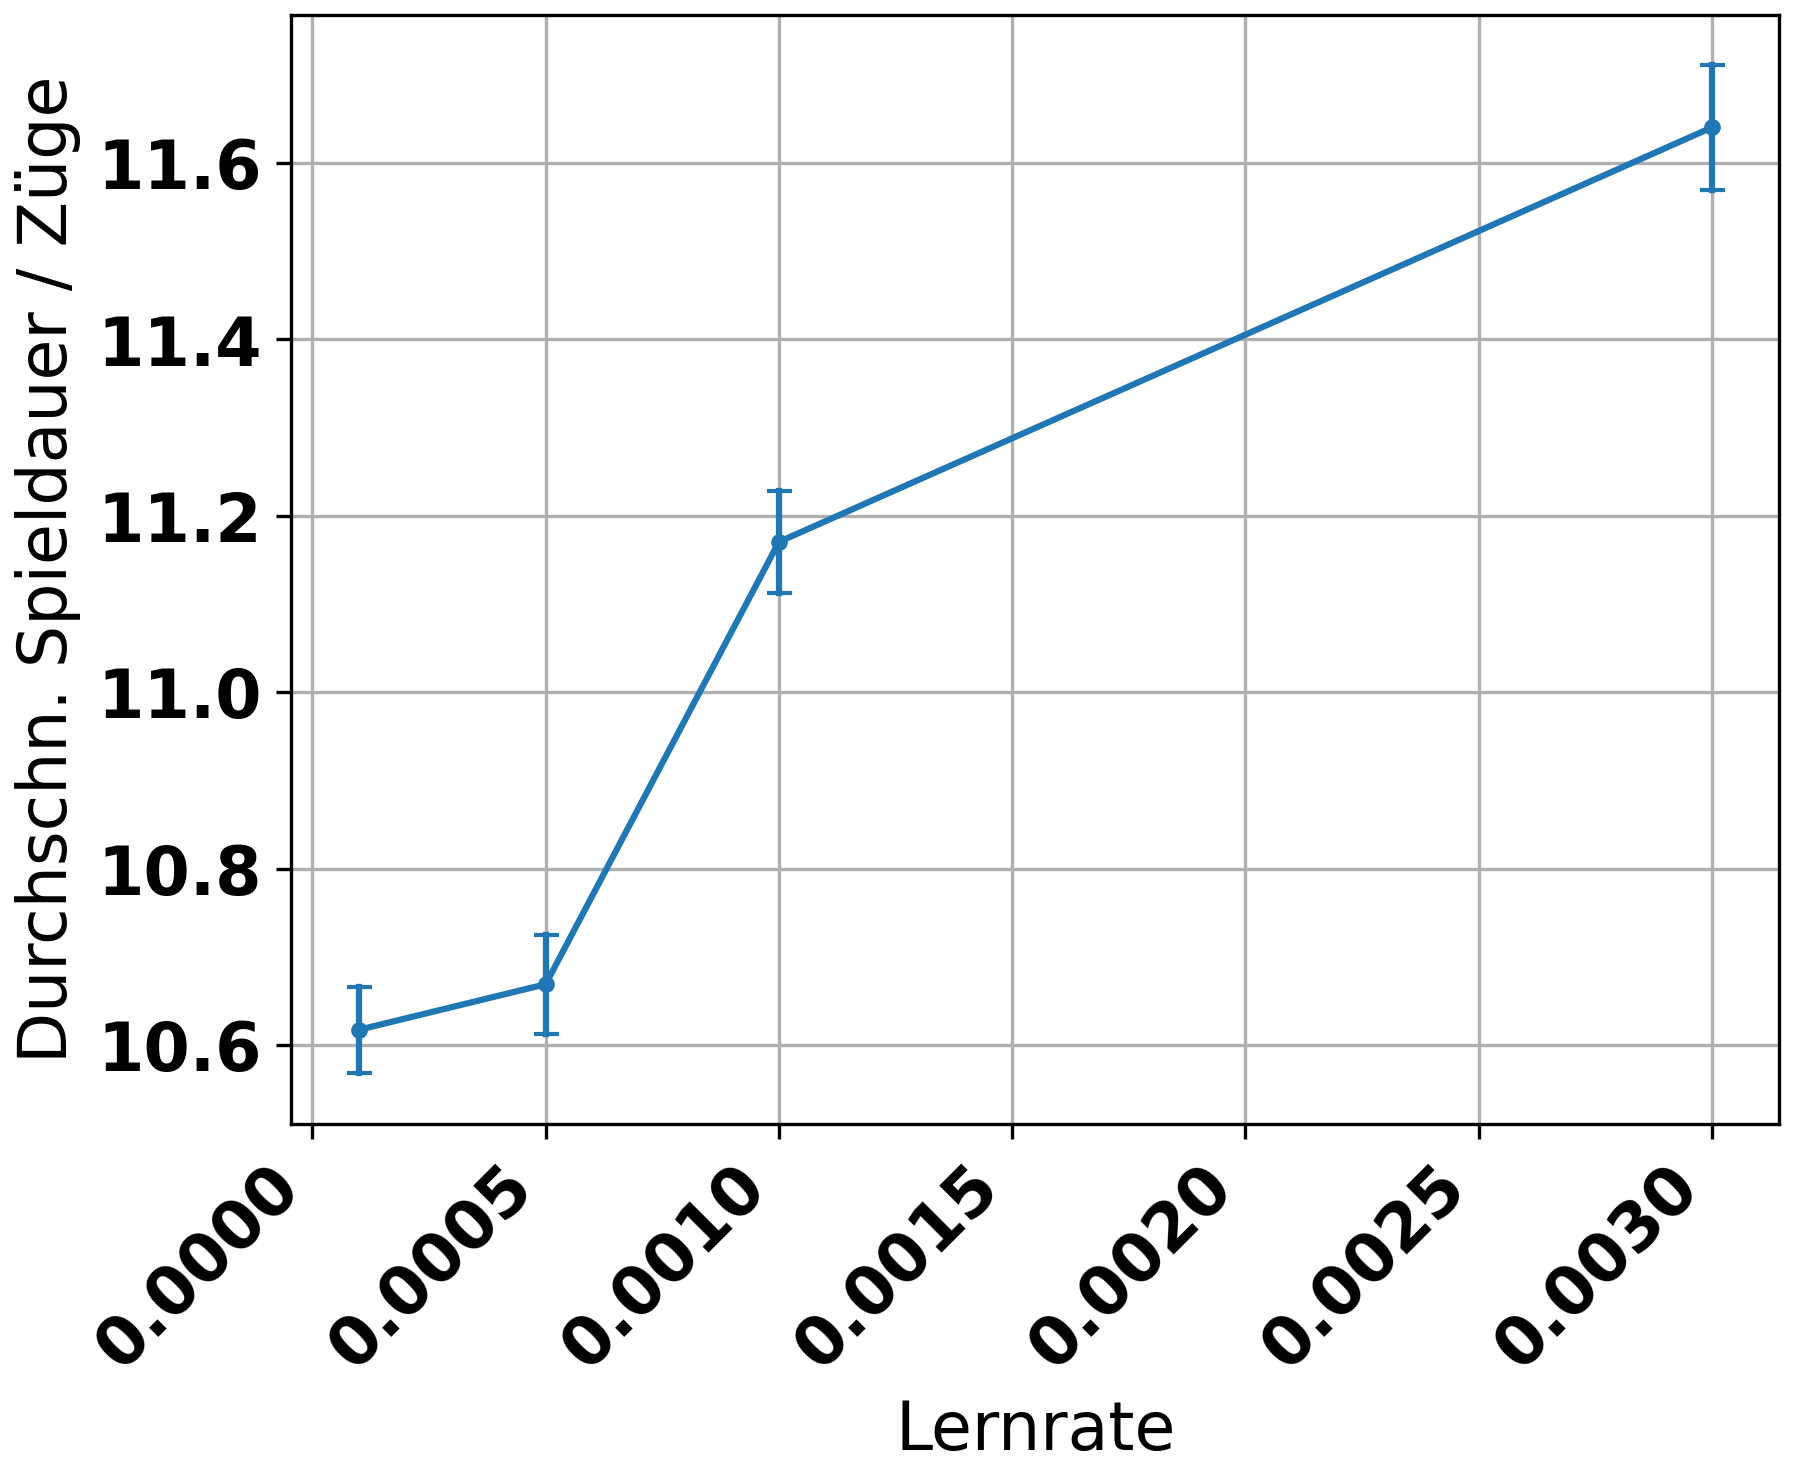
\includegraphics[width=\textwidth]{Bilder/ppo_vs_random_game_length_vs_learning_rate.png}
		\caption{Durchschnittliche Spieldauer.}
		\label{fig:f22}
	\end{subfigure}
	\caption{Gewinnrate und durchschnittliche Spieldauer in Abhängigkeit von der Lernrate beim Training eines PPO-Modells gegen einen zufällig spielenden Agenten.}
\end{figure}

Um die Leistung der trainierten Modelle gegen den zufällig spielenden Agenten zu evaluieren, wurden mit jedem Modell 20.000 Spiele durchgeführt und die Gewinnrate und Spieldauer wurde aufgezeichnet. Mit steigender Lernrate sinkt die durch das trainierte Modell erzielte Gewinnrate stetig von 97,3 \% (95 \%-CI: 97,1 - 97,6) auf 89,3 \% (95 \%-CI: 88,9 - 89,7) und die durchschnittliche Spieldauer steigt von 10,62 Zügen (95 \%-CI: 10,57 - 10,67) auf 11,64 Züge (95 \%-CI: 11,57 - 11,71). Durch das Training mit kleineren Lernraten werden damit bessere Ergebnisse erzielt, wobei die Verbesserungen mit kleiner werdender Lernrate immer geringfügiger werden. Das Training mit weiteren kleineren Lernraten bleibt daher im Rahmen dieser Arbeit erspart. Für die weiteren Untersuchungen kommt das Modell zum Einsatz, das aus dem Training mit der Lernrate $\alpha_3$ entstanden ist.

Wie beim MCTS-Agenten wurde eine einfache qualitative Analyse im Spiel gegen einen Menschen durchgeführt, um ein Bild von der Strategie des trainierten PPO-Agenten zu bekommen. Daraus geht hervor, dass der PPO-Agent stets als erstes das unterste Feld in der mittleren Spalte besetzt, wenn er dazu die Möglichkeit hat, was wie in Kapitel \ref{qualitative-untersuchung} bereits erwähnt, der stärkste Anfangszug ist. Der PPO-Agent tendiert dazu, seine Spielsteine vertikal zu stapeln, in manchen Fällen baut er auch horizontale Ketten. Wenn er drei Spielsteine in einer Kette platziert hat, setzt er meistens auch den vierten Stein zum Gewinnen, wenn dies möglich ist. Er blockiert hingegen äußerst selten seinen Gegenspieler, wenn er droht, in seinem nächsten Zug das Spiel für sich zu entscheiden. So ist es als Mensch sehr einfach möglich, gegen den RL-Agenten zu gewinnen, beispielsweise indem man selbst seine Steine in einer Spalte stapelt und von dieser Strategie nur abweicht, um den PPO-Agenten daran zu hindern, den vierten Stein in eine seiner Ketten zu platzieren.

Die in der quantitativen Analyse ermittelte Gewinnrate und Spieldauer des PPO-Agenten liegt mit 97,3 \% (95 \%-CI: 97,1 - 97,6) bzw. 10,62 Zügen (95 \%-CI: 10,57 - 10,67) nahe bei den durch den MCTS-Agenten erzielten Werten von 100 \% (95 \%-CI: 98,1 - 100,0) bzw. 9,72 Zügen (95 \%-CI: 9,32 - 10,12). Es scheint, als wären die Agenten ähnlich stark. Aus der qualitativen Analyse geht jedoch hervor, dass der MCTS-Agent eine langfristig ausgerichtete Strategie verfolgt, die auch gegen zielgerichtete Gegenspieler standhalten kann, während der PPO-Agent auf kurzfristige Gewinne abzielt, wodurch er mit einfachen Mitteln besiegt werden kann. Die kurzfristig ausgerichtete Strategie des PPO-Agenten entsteht dadurch, dass sie ausreicht, um im Training gegen den zufällig spielenden Agenten in den meisten Fällen zu gewinnen, sodass kein Lernanreiz für Strategien besteht, die auch gegen intelligentere Gegenspieler funktionieren.

Die im Konzept geforderte Bedingung, dass die zu untersuchenden Agenten gleich stark sein müssen, um aussagekräftige Aussagen über die Robustheit der Verfahren zu äußern, konnte somit weiterhin nicht erfüllt werden. Es ist davon auszugehen, dass der implementierte RL-Agent alleine aufgrund seiner unterlegenen Spielstrategie auch in den Untersuchungen zur Robustheit schlechter abschneiden wird. Die Untersuchungen bezüglich Robustheit werden dennoch weiter fortgesetzt, denn noch ist nicht ausgeschlossen, dass der implementierte PPO-Agent entgegen der Erwartungen bessere Ergebnisse erzielt als der MCTS-Agent.

\subsection{Szenarien zur Untersuchung von Robustheit}

\label{robustheit-szenarien}

Um die im Konzept genannten Szenarien zu implementieren, wurde die Messumgebung um eine Klasse \texttt{DistortionGenerator} erweitert. Über dessen Konstruktor können zwei Attribute gesetzt werden, eines um die Wahrscheinlichkeit festzulegen, mit der eine Aktion verfälscht werden soll, und ein Weiteres um die Anzahl von falsch zu beobachtenden Feldern zu konfigurieren.


\begingroup

\emergencystretch 5em%

	 Sie besitzt eine Methode \texttt{distort\char`_action(orinal\char`_action: int, action\char`_mask: list[int]) -> int}, die eine von einem Agenten gewählte Aktion und die im aktuellen Zustand möglichen Aktionen entgegennimmt, und mit der im Konstruktor gegebenen Wahrscheinlichkeit eine zufällige Aktion und ansonsten die ursprüngliche Aktion zurückgibt. Sie wird immer dann ausgeführt, nachdem die Messumgebung für einen Agenten einen Zug berechnet hat und es wird die Aktion ausgeführt, die durch diese Funktion zurückgegeben wird.

	Die Methode \texttt{distort\char`_state(state: numpy.ndarray(6, 7, 2)) -> numpy.ndarray(6, 7, 2)} nimmt den aktuellen Zustand des Spielfelds entgegen. Sie verwaltet zwei Listen, die jeweils Koordinaten von Spielfeldern enthalten. Eine Liste für Felder, bei denen Steiner platziert, und eine weitere Liste für Felder, bei denen Steine entfernt werden können, sodass jeweils illegale Zustände entstehen. In die erste Liste werden die Felder hinzugefügt, dessen unteren Nachbarn frei sind, und in die zweite Liste werden die Felder hinzugefügt, dessen obere Nachbarn besetzt sind. Wie in Kapitel \ref{konzept} erwähnt, wird dabei beachtet, dass aus vollen Spalten keine Spielsteine entfernt werden und keine Spalten mit nur einem freien Feld gefüllt werden, sodass sich die im beobachteten Zustand möglichen Aktionen nicht von den im tatsächlichen Zustand möglichen Aktionen unterscheiden. Die Methode wird nach jedem Spielzug durchgeführt, sobald der neue Zustand des Spielfelds bekannt ist. Das Ergebnis wird an die Agenten weitergegeben, die auf dessen Grundlage den nächsten Zug wählen.

\endgroup

Eine Frage, die sich bei der Implementierung des Szenarios Unsicherheit bezüglich Beobachtungen stellt, ist wie der MCTS-Agent auf Grundlage des illegalen Spielfeldzustands Simulationen durchführt. Durch die in dieser Implementierung eingesetzte PettingZoo-Umgebung, wird der Fall, dass ein Stein in eine Spalte platziert wird, in der sich ein Stein über einem freien Feld befindet, so gehandhabt, dass der zu platzierende Stein im untersten freien Feld landet. Eine alternative Herangehensweise wäre, den zu platzierenden Stein immer auf das freie Feld über das höchste besetzte Feld zu setzen. Es wird angenommen, dass die beiden Herangehensweisen keinen wesentlichen Unterschied in der Leistungsfähigkeit des MCTS-Agenten verursachen, daher wird das Verhalten so belassen, wie es in der PettingZoo-Umgebung umgesetzt ist.

Es war jedoch eine Anpassung an das Action Masking der PettingZoo-Umgebung notwendig, also der Art und Weise, wie in berechnet wird, welche Aktionen möglich sind. Diese Berechnung ist so implementiert, dass Spalten als nicht bespielbar gekennzeichnet werden, sobald das oberste Feld der Spalte belegt ist. Das bedeutet, wenn fälschlicherweise beobachtet wird, dass das oberste Feld einer Spalte besetzt ist, wird sie als nicht bespielbar gekennzeichnet, auch wenn darunter freie Felder beobachtet werden. Das Action Masking wurde daher so angepasst, dass Spalten erst dann als nicht bespielbar gekennzeichnet werden, wenn alle Felder in der Spalte besetzt sind.
